\documentclass[11pt,a4paper]{article}
\usepackage[margin=2.2cm]{geometry}
\usepackage{graphicx}
\usepackage{booktabs}
\usepackage{longtable}
\usepackage{array}
\usepackage{multirow}
\usepackage{siunitx}
\usepackage{xcolor}
\usepackage{caption}
\usepackage{subcaption}
\usepackage{float}
\usepackage{hyperref}
\usepackage{amsmath}
\usepackage{enumitem}
\usepackage{tabularx}
\usepackage{adjustbox}
\usepackage{microtype}
\usepackage{tikz}
\usetikzlibrary{arrows.meta,positioning,shapes.misc,calc,fit,backgrounds}
\usepackage[edges]{forest}
\usepackage{pdflscape}
\hypersetup{colorlinks=true,linkcolor=blue!60!black,urlcolor=blue!60!black}
\graphicspath{{figures/}}
\captionsetup{font=small,labelfont=bf}
\newcommand{\code}[1]{\texttt{\small #1}}
\newcommand{\good}[1]{\textcolor{green!50!black}{#1}}
\newcommand{\bad}[1]{\textcolor{red!70!black}{#1}}
\newcommand{\Umag}{|U|}

\title{ISDA 2026 experiments --- results overview\\
\large ESMDA, sequential filtering (EnKF), and filter smoothing on the Xie \& Castro urban case}
\author{Generated from \code{presentations/isda\_new/experiments/}}
\date{\today}

\begin{document}
\maketitle
\tableofcontents
\clearpage

\section{Experimental design common to all campaigns}
\label{sec:setup}

All experiments were produced by the three driver campaigns under
\code{presentations/isda\_new/experiments/} (\code{esmda/}, \code{filtering/},
\code{filter\_smoothing/}) and share one physical set-up. The three campaigns differ only
in the assimilation algorithm and in which knobs are swept. This section records the
shared configuration once so that the method sections can focus on results.

\subsection{Case, domain and models}
\begin{itemize}[nosep]
  \item \textbf{Geometry}: Xie \& Castro (2008) staggered-cube urban array,
        \code{examples/xie\_and\_castro/xie\_castro\_2008\_STL.stl}.
  \item \textbf{Domain}: $40\times60\times16$ cells over
        $x\in[-20,40]$, $y\in[0,80]$, $z\in[0,32]$~m (2~m resolution).
  \item \textbf{Assimilation model}: uDALES (\code{pyudales}) with Vreman closure in every run.
  \item \textbf{Truth model}: either uDALES (\emph{matched model}, primary case) or PALM
        (\code{pypalm}, \emph{model-error} case). Truth trajectories are stored in
        \code{experiments/truth\_states/true\_state\_<truth>\_<case>.nc}.
  \item \textbf{Boundary-condition cases}:
        \code{inflow} = laminar inlet (\code{inlet\_turbulence.enabled=false});
        \code{inflow\_turb} = synthetic turbulent inlet (intensity 0.05, length scale 6~m);
        \code{periodic} = periodic lateral boundaries.
  \item \textbf{Time}: 3 assimilation windows $\times$ 120~s $=$ 360~s; 50~s spin-up;
        model output every 2~s.
\end{itemize}

\subsection{Parameters, truth and prior}
Two time-varying inflow parameters are estimated (one knot per 30~s, i.e.\ 15 knots over
360~s); the vertical inflow exponent is a static nuisance parameter.
\begin{center}\small
\begin{tabular}{lll}
\toprule
Parameter & Truth (deterministic sinusoid) & Prior (AR(2) relaxation, $L_\mathrm{corr}=200$~s) \\
\midrule
Inflow angle $\alpha$ & $20^\circ\sin(2\pi t/300\,\mathrm{s})$ & $\mathcal N(0^\circ, 10^\circ)$ \\
Velocity magnitude $\Umag$ & $7.5 + 1.0\,\sin(2\pi t/150\,\mathrm{s})$~m/s & $\mathcal N(7.5, 0.5)$~m/s \\
Vertical exponent & $0.25$ (constant) & $\mathcal N(0.25, 0.05)$ \\
\bottomrule
\end{tabular}
\end{center}
A climatological (prior-only) angle estimate therefore scores $\approx 17$--$20^\circ$
RMSE; that is the baseline every ``reduction vs.\ prior'' is measured against.

\subsection{Observations}
\begin{itemize}[nosep]
  \item \textbf{Assimilated sensors} (6, all at $z=2$~m): $(10,20)$, $(10,60)$, $(20,10)$,
        $(20,50)$, $(30,30)$, $(30,70)$; observed components $u$ and $v$;
        $\sigma_\mathrm{obs}=0.1$~m/s.
  \item \textbf{Validation sensors} (4, never assimilated): $(2,30,2)$, $(20,55,2)$,
        $(17,30,2)$ and one elevated sensor $(10,30,20)$.
  \item \textbf{Ensemble}: $N=50$ members, 10 parallel processes.
  \item \textbf{Localization} (\code{loccorrelation}): correlation-based localization
        (truncation 0.35, tapering $\beta=0.5$, max inflation 8, block grouping);
        \code{locnone} = no localization.
\end{itemize}

\subsection{Naming convention}
Run folders are named
\code{<truth>\_to\_<assim>\_w3\_<loc>[\_obs<interval>]\_<case>[\_state\_infl<none|rtps>]}, where
\code{w3} = three windows, \code{obs7p5/obs15/obs30} = observation aggregation interval in
seconds (ESMDA and filter smoothing only), and the optional \code{\_state\_infl*} suffix marks
state-only filtering runs with the given inflation.

\subsection{Metrics}
\begin{description}[nosep]
  \item[Parameter RMSE / CRPS] ensemble-mean error and CRPS of each parameter against truth,
        averaged over knots (``mean'') or at the last knot (``final''). \emph{Reduction vs.\
        prior} is relative to the same run's own prior ensemble.
  \item[Sensor vector RMSE] $\sqrt{\sum_{c\in\{u,v,w\}}\mathrm{RMSE}_c^2}$ of the ensemble
        mean at the assimilated (\emph{assim}) or held-out (\emph{valid}) sensors. Note that
        figure legends print a \emph{magnitude-only} $\Umag$ RMSE, which is systematically
        smaller than the vector RMSE quoted in the tables.
  \item[Energy score (ES)] multivariate CRPS of the sensor velocity vector.
  \item[State RMSE] domain-wide RMSE of $\Umag$ of the ensemble mean vs.\ truth.
  \item[Data mismatch $O_N$] (ESMDA) normalised observation misfit; the noise floor is
        $O_N=1/2$.
  \item[Calibration] $z$-score standard deviation of parameter errors (1.03 expected for
        $N=50$; $\gg 1$ = overconfident), contraction ratio (posterior/prior spread),
        rank histograms, innovation $\chi^2$ (filters; 1 = calibrated), and field hit rate
        $q$ (fraction of grid points where truth lies inside the ensemble envelope).
\end{description}

\subsection{Compute}
Each campaign was driven sequentially by \code{\_chain*/chain\_progress.tsv}. Approximate
wall time per method (all runs of one truth model): ESMDA 8--13~h, filtering 7--9~h,
filter smoothing 11--17~h; individual runs take 1--2.5~h on 10 processes.

\clearpage
% ESMDA section.
% Tables are auto-generated: experiments_report/scripts/extract_esmda.py
%   -> sections/esmda_tables.tex (\EsmdaMatrixTable, \EsmdaMasterTable, \EsmdaCalibTable)
% Figures are auto-generated: experiments_report/scripts/make_esmda_figures.py
%   -> figures/esmda/

\begingroup\sloppy

\section{ESMDA}
\label{sec:esmda}

% AUTO-GENERATED by experiments_report/scripts/extract_esmda.py
% Do not edit by hand; re-run the script instead.
% 20 runs, 18 completed, 2 failed.

\newcommand{\EsmdaMatrixTable}{%
\begin{table}[htbp]
\centering
\caption{ESMDA: experiment matrix. Twenty configurations; the observation
interval is the method knob. \emph{loc} is localization on
(\code{loccorrelation}) or off (\code{locnone}). Run-directory names are given
here only; everywhere else runs are cited by ID. The two failed runs died in the
PALM \emph{truth} simulation before any assimilation started
(Section~\ref{sec:esmda-failed}).}
\label{tab:esmda-matrix}
\footnotesize
\begin{adjustbox}{max width=\textwidth}
\begin{tabular}{llllcc l}
\toprule
ID & run directory & truth & case & loc & obs [s] & status \\
\midrule
E1 & \code{pypalm\_to\_pyudales\_w3\_loccorrelation\_obs15\_inflow} & PALM & \code{inflow} & on & 15 & failed (truth run) \\
E2 & \code{pypalm\_to\_pyudales\_w3\_loccorrelation\_obs15\_inflow\_turb} & PALM & \code{inflow\_turb} & on & 15 & ok \\
E3 & \code{pypalm\_to\_pyudales\_w3\_loccorrelation\_obs15\_periodic} & PALM & \code{periodic} & on & 15 & ok \\
E4 & \code{pypalm\_to\_pyudales\_w3\_loccorrelation\_obs30\_inflow\_turb} & PALM & \code{inflow\_turb} & on & 30 & ok \\
E5 & \code{pypalm\_to\_pyudales\_w3\_loccorrelation\_obs30\_periodic} & PALM & \code{periodic} & on & 30 & ok \\
E6 & \code{pypalm\_to\_pyudales\_w3\_loccorrelation\_obs7p5\_inflow\_turb} & PALM & \code{inflow\_turb} & on & 7.5 & ok \\
E7 & \code{pypalm\_to\_pyudales\_w3\_loccorrelation\_obs7p5\_periodic} & PALM & \code{periodic} & on & 7.5 & ok \\
E8 & \code{pypalm\_to\_pyudales\_w3\_locnone\_obs15\_inflow} & PALM & \code{inflow} & off & 15 & failed (truth run) \\
E9 & \code{pypalm\_to\_pyudales\_w3\_locnone\_obs15\_inflow\_turb} & PALM & \code{inflow\_turb} & off & 15 & ok \\
E10 & \code{pypalm\_to\_pyudales\_w3\_locnone\_obs15\_periodic} & PALM & \code{periodic} & off & 15 & ok \\
\midrule
E11 & \code{pyudales\_to\_pyudales\_w3\_loccorrelation\_obs15\_inflow} & uDALES & \code{inflow} & on & 15 & ok \\
E12 & \code{pyudales\_to\_pyudales\_w3\_loccorrelation\_obs15\_inflow\_turb} & uDALES & \code{inflow\_turb} & on & 15 & ok \\
E13 & \code{pyudales\_to\_pyudales\_w3\_loccorrelation\_obs15\_periodic} & uDALES & \code{periodic} & on & 15 & ok \\
E14 & \code{pyudales\_to\_pyudales\_w3\_loccorrelation\_obs30\_inflow\_turb} & uDALES & \code{inflow\_turb} & on & 30 & ok \\
E15 & \code{pyudales\_to\_pyudales\_w3\_loccorrelation\_obs30\_periodic} & uDALES & \code{periodic} & on & 30 & ok \\
E16 & \code{pyudales\_to\_pyudales\_w3\_loccorrelation\_obs7p5\_inflow\_turb} & uDALES & \code{inflow\_turb} & on & 7.5 & ok \\
E17 & \code{pyudales\_to\_pyudales\_w3\_loccorrelation\_obs7p5\_periodic} & uDALES & \code{periodic} & on & 7.5 & ok \\
E18 & \code{pyudales\_to\_pyudales\_w3\_locnone\_obs15\_inflow} & uDALES & \code{inflow} & off & 15 & ok \\
E19 & \code{pyudales\_to\_pyudales\_w3\_locnone\_obs15\_inflow\_turb} & uDALES & \code{inflow\_turb} & off & 15 & ok \\
E20 & \code{pyudales\_to\_pyudales\_w3\_locnone\_obs15\_periodic} & uDALES & \code{periodic} & off & 15 & ok \\
\bottomrule
\end{tabular}
\end{adjustbox}
\end{table}%
}

\newcommand{\EsmdaMasterTable}{%
\begin{table}[htbp]
\centering
\caption{ESMDA: master results for all 20 runs, uDALES-truth block above,
PALM-truth block below. \emph{assim} / \emph{valid} are the vector RMSE
[m/s] of the ensemble mean at the 6 assimilated and 4 validation sensors,
averaged over time; \emph{field} $\Umag$ is the domain-wide RMSE of the velocity
magnitude. The two parameter columns give the knot-mean RMSE with the reduction
vs.\ prior in parentheses (priors are re-drawn per run, so only the reduction is
comparable across rows, and never across methods). ESMDA has no sequential
innovation, so $\chi^2$ is undefined; $z_{\mathrm{par}}$ is the pooled parameter
$z$-score standard deviation (1.03 = calibrated); $q$ is the field hit rate
(uDALES truth only). Bold = best in the column within the truth block; $q$ and
$\chi^2$ are not bolded.}
\label{tab:esmda-master}
\footnotesize
\begin{adjustbox}{max width=\textwidth}
\begin{tabular}{llcc rrr rr rrr r}
\toprule
 & & & obs & \multicolumn{2}{c}{vector RMSE [m/s]} & field & \multicolumn{2}{c}{parameter RMSE (red.\%)} & & & & wall \\
\cmidrule(lr){5-6}\cmidrule(lr){8-9}
ID & case & loc & [s] & assim & valid & $\Umag$ & $\alpha$ [deg] & $\Umag$ [m/s] & $\chi^2$ & $z_{\mathrm{par}}$ & $q$ & [h] \\
\midrule
E11 & \code{inflow} & on & 15 & 0.665 & 0.748 & 0.477 & 7.74 (61) & 0.529 (31) & -- & 12.1 & 0.72 & 2.19 \\
E18 & \code{inflow} & off & 15 & 0.694 & 0.754 & 0.521 & 7.59 (62) & 0.671 (18) & -- & 13.6 & 0.72 & 2.15 \\
E16 & \code{inflow\_turb} & on & 7.5 & 0.439 & 0.422 & 0.408 & 2.42 (86) & 0.379 (51) & -- & 6.1 & 0.74 & 2.24 \\
E12 & \code{inflow\_turb} & on & 15 & \textbf{0.401} & \textbf{0.365} & \textbf{0.372} & \textbf{2.31} (87) & \textbf{0.369} (53) & -- & 4.6 & 0.62 & 2.30 \\
E19 & \code{inflow\_turb} & off & 15 & 0.456 & 0.407 & 0.421 & 2.45 (87) & 0.439 (42) & -- & 7.8 & 0.62 & 2.29 \\
E14 & \code{inflow\_turb} & on & 30 & 0.418 & 0.366 & 0.388 & 2.35 (87) & 0.414 (48) & -- & 4.1 & 0.80 & 2.27 \\
E17 & \code{periodic} & on & 7.5 & 1.104 & 1.394 & 1.056 & 12.94 (18) & 0.754 (7) & -- & 3.3 & 0.84 & 1.73 \\
E13 & \code{periodic} & on & 15 & 1.091 & 1.408 & 1.040 & 13.62 (18) & 0.717 (9) & -- & 2.6 & 0.71 & 1.77 \\
E20 & \code{periodic} & off & 15 & 1.163 & 1.671 & 1.075 & 14.84 (22) & 0.764 (4) & -- & 89.8 & 0.58 & 1.80 \\
E15 & \code{periodic} & on & 30 & 1.089 & 1.417 & 1.033 & 13.63 (19) & 0.748 (7) & -- & 2.5 & 0.70 & 1.76 \\
\midrule
E1 & \code{inflow} & on & 15 & \multicolumn{9}{c}{\emph{failed (truth run)}} \\
E8 & \code{inflow} & off & 15 & \multicolumn{9}{c}{\emph{failed (truth run)}} \\
E6 & \code{inflow\_turb} & on & 7.5 & 1.432 & 1.327 & \textbf{1.024} & 7.83 (47) & \textbf{0.432} (41) & -- & 13.9 & -- & 2.24 \\
E2 & \code{inflow\_turb} & on & 15 & \textbf{1.422} & 1.377 & 1.082 & 7.12 (58) & 0.472 (40) & -- & 12.5 & -- & 2.36 \\
E9 & \code{inflow\_turb} & off & 15 & 1.481 & 1.389 & 1.050 & \textbf{6.62} (60) & 0.561 (30) & -- & 18.4 & -- & 2.35 \\
E4 & \code{inflow\_turb} & on & 30 & 1.429 & \textbf{1.323} & 1.068 & 7.44 (50) & 0.524 (35) & -- & 9.6 & -- & 2.30 \\
E7 & \code{periodic} & on & 7.5 & 1.495 & 1.806 & 4.033 & 14.86 (14) & 1.016 (-10) & -- & 3.2 & -- & 1.99 \\
E3 & \code{periodic} & on & 15 & 1.437 & 2.133 & 4.014 & 22.42 (-10) & 1.090 (-15) & -- & 3.1 & -- & 2.08 \\
E10 & \code{periodic} & off & 15 & 1.575 & 1.960 & 4.487 & 16.19 (2) & 1.602 (-36) & -- & 263.3 & -- & 2.17 \\
E5 & \code{periodic} & on & 30 & 1.438 & 1.941 & 4.190 & 15.86 (10) & 1.418 (-24) & -- & 3.2 & -- & 2.13 \\
\bottomrule
\end{tabular}
\end{adjustbox}
\end{table}%
}

\newcommand{\EsmdaCalibTable}{%
\begin{table}[htbp]
\centering
\caption{ESMDA: calibration diagnostics. $\chi^2$ is undefined for a smoother.
std$(z)$ is the standard deviation of the per-knot parameter $z$-scores
$(\theta^\ast-\bar\theta^a)/\sigma^a$; a calibrated 50-member ensemble gives
1.03, so every entry is over-confident. \emph{Contraction} is the knot-mean
posterior/prior spread ratio ($\ll 1$ = the data informed the parameter,
$\approx 1$ = unidentifiable). $q$ and its per-component values are field hit
rates (uDALES truth only). \emph{rank edge frac} is the fraction of the
validation-sensor rank histogram falling in the two outer bins; a calibrated
51-bin histogram gives 0.04.}
\label{tab:esmda-calib}
\footnotesize
\begin{adjustbox}{max width=\textwidth}
\begin{tabular}{llcc r rrr rr rrrr r}
\toprule
 & & & obs & & \multicolumn{3}{c}{std$(z)$} & \multicolumn{2}{c}{contraction} & \multicolumn{4}{c}{field hit rate} & rank edge \\
\cmidrule(lr){6-8}\cmidrule(lr){9-10}\cmidrule(lr){11-14}
ID & case & loc & [s] & $\chi^2$ & $\alpha$ & $\Umag$ & pool & $\alpha$ & $\Umag$ & $q$ & $u$ & $v$ & $w$ & frac (valid) \\
\midrule
E11 & \code{inflow} & on & 15 & -- & 12.9 & 11.5 & 12.1 & 0.30 & 0.37 & 0.72 & 0.93 & 0.73 & 0.50 & 0.50 \\
E18 & \code{inflow} & off & 15 & -- & 13.9 & 13.7 & 13.6 & 0.30 & 0.35 & 0.72 & 0.93 & 0.75 & 0.50 & 0.58 \\
E16 & \code{inflow\_turb} & on & 7.5 & -- & 5.2 & 7.0 & 6.1 & 0.23 & 0.36 & 0.74 & 0.94 & 0.65 & 0.61 & 0.75 \\
E12 & \code{inflow\_turb} & on & 15 & -- & 3.0 & 5.8 & 4.6 & 0.24 & 0.36 & 0.62 & 0.94 & 0.30 & 0.62 & 0.58 \\
E19 & \code{inflow\_turb} & off & 15 & -- & 4.5 & 10.2 & 7.8 & 0.22 & 0.29 & 0.62 & 0.94 & 0.30 & 0.62 & 0.33 \\
E14 & \code{inflow\_turb} & on & 30 & -- & 2.3 & 5.4 & 4.1 & 0.25 & 0.40 & 0.80 & 0.94 & 0.83 & 0.62 & 0.25 \\
E17 & \code{periodic} & on & 7.5 & -- & 3.0 & 3.6 & 3.3 & 0.59 & 0.71 & 0.84 & 0.93 & 0.88 & 0.70 & 0.17 \\
E13 & \code{periodic} & on & 15 & -- & 2.3 & 2.8 & 2.6 & 0.67 & 0.74 & 0.71 & 0.93 & 0.47 & 0.71 & 0.00 \\
E20 & \code{periodic} & off & 15 & -- & 91.9 & 88.8 & 89.8 & 0.19 & 0.19 & 0.58 & 0.88 & 0.21 & 0.64 & 0.17 \\
E15 & \code{periodic} & on & 30 & -- & 2.2 & 2.8 & 2.5 & 0.69 & 0.75 & 0.70 & 0.92 & 0.47 & 0.71 & 0.08 \\
\midrule
E1 & \code{inflow} & on & 15 & \multicolumn{11}{c}{\emph{failed (truth run)}} \\
E8 & \code{inflow} & off & 15 & \multicolumn{11}{c}{\emph{failed (truth run)}} \\
E6 & \code{inflow\_turb} & on & 7.5 & -- & 16.2 & 8.1 & 13.9 & 0.23 & 0.34 & -- & -- & -- & -- & 0.83 \\
E2 & \code{inflow\_turb} & on & 15 & -- & 13.3 & 7.0 & 12.5 & 0.24 & 0.37 & -- & -- & -- & -- & 0.83 \\
E9 & \code{inflow\_turb} & off & 15 & -- & 20.3 & 15.3 & 18.4 & 0.21 & 0.29 & -- & -- & -- & -- & 0.92 \\
E4 & \code{inflow\_turb} & on & 30 & -- & 10.1 & 6.3 & 9.6 & 0.25 & 0.39 & -- & -- & -- & -- & 0.67 \\
E7 & \code{periodic} & on & 7.5 & -- & 2.8 & 3.5 & 3.2 & 0.65 & 0.65 & -- & -- & -- & -- & 0.25 \\
E3 & \code{periodic} & on & 15 & -- & 3.3 & 2.8 & 3.1 & 0.64 & 0.80 & -- & -- & -- & -- & 0.25 \\
E10 & \code{periodic} & off & 15 & -- & 173.2 & 326.6 & 263.3 & 0.16 & 0.16 & -- & -- & -- & -- & 0.33 \\
E5 & \code{periodic} & on & 30 & -- & 3.0 & 3.3 & 3.2 & 0.65 & 0.82 & -- & -- & -- & -- & 0.33 \\
\bottomrule
\end{tabular}
\end{adjustbox}
\end{table}%
}


\subsection{Method and experiment matrix}
\label{sec:esmda-method}

ESMDA is run here as \code{TimeVaryingParameterESMDA} with
\code{joint\_state\_and\_parameter: false}, i.e.\ a \emph{parameter-only}
smoother. The state is never touched by the analysis: it improves only because
the forward model is re-run over the whole window with better boundary
parameters. Each of the three \SI{120}{\second} windows is solved with 3 ESMDA
iterations at inflation $\alpha_i = 3$ --- four forward ensemble passes per
window --- and is warm-started from the previous window's final state. The
control vector is the pair of time-varying inflow parameters $\alpha$ and
$\Umag$ on 15 harmonic knots (\SI{30}{\second} per knot, window boundaries
sharing a knot); \code{pin\_initial\_time\_point: true}, and the static vertical
inflow exponent is not estimated. Observations are time-mean aggregates of $u$
and $v$ over the observation interval, so the observation count per window is
$N_d = 192 / 96 / 48$ at $\Delta t_{\mathrm{obs}} = 7.5 / 15 / \SI{30}{\second}$.

Two knobs are swept. The \textbf{observation interval} is the method knob of
this section; localization on/off is the shared knob. Localization was varied
only at $\Delta t_{\mathrm{obs}} = \SI{15}{\second}$ and the interval only on
\code{inflow\_turb} and \code{periodic}, so the twenty configurations of
Table~\ref{tab:esmda-matrix} form a cross, not a full grid. The reference run of
each case is uDALES truth with localization on at
$\Delta t_{\mathrm{obs}} = \SI{15}{\second}$: E11 (\code{inflow}),
E12 (\code{inflow\_turb}), E13 (\code{periodic}).

One ESMDA-specific diagnostic is quoted throughout and appears in no table: the
normalised data mismatch $O_N$ (median over members) after each iteration, whose
nominal target is $1/2$. Every run is flagged \code{underfit\_final: true} with
\code{caveat: no\_representativeness\_error}, so only the \emph{trend} across
iterations is meaningful, and $O_N$ is not comparable between observation
intervals because $N_d$ differs.

\EsmdaMatrixTable

\subsection{Master results}
\label{sec:esmda-master}

\EsmdaMasterTable

Table~\ref{tab:esmda-master} collects every run. Read as a block it says four
things. First, the \emph{case} dominates every knob: with uDALES truth the
$\alpha$ RMSE is 2.31--\SI{2.45}{\degree} on \code{inflow\_turb},
7.59--\SI{7.74}{\degree} on \code{inflow} and 12.9--\SI{14.8}{\degree} on
\code{periodic}, while localization and the observation interval move it by
tenths of a degree. Second, that ordering \emph{inverts} the naive one: the
physically harder turbulent-inlet case is the one ESMDA does best on, because
there the boundary forcing --- and hence the estimated parameters --- is what
the sensors actually see. Third, the truth model matters almost as much as the
case: the same \code{inflow\_turb} configuration under PALM truth only reaches
6.62--\SI{7.83}{\degree}, and the field $\Umag$ RMSE degrades from
$\approx 0.37$ to $\approx 1.05$. Fourth, ESMDA \good{generalises at least as
well as it fits} wherever it works at all --- on E12 the validation vector RMSE
(0.365) is \emph{below} the assimilation vector RMSE (0.401), the expected
signature of correcting a global boundary condition rather than local state.

Two cautions on reading the table. The reduction-vs-prior percentages are
relative to each run's own re-drawn prior (\SI{14.6}{\degree} to
\SI{20.3}{\degree} of $\alpha$ RMSE across the set), so they compare rows within
this section but must never be carried across methods. And on \code{periodic}
the 18--22\,\% ``reduction'' is a spread reduction, not a bias reduction
(Section~\ref{sec:esmda-periodic}).

\subsection{Results by case}
\label{sec:esmda-cases}

This subsection uses uDALES truth only; PALM truth is
Section~\ref{sec:esmda-modelerror}.

\subsubsection{Laminar inflow (\code{inflow})}
\label{sec:esmda-inflow}

\begin{figure}[htbp]
\centering
\includegraphics[width=\textwidth]{esmda/valid_E11.png}
\caption{E11 (uDALES truth, \code{inflow}, localization on,
$\Delta t_{\mathrm{obs}} = \SI{15}{\second}$): validation sensors 0
($z = \SI{2}{\meter}$) and 3 ($z = \SI{20}{\meter}$, never observed at that
height) and the pooled validation error. The ensemble tracks truth almost
exactly for the first \SI{120}{\second}, then loses phase: the error rises from
$< 0.2$ to $1.7$ around $t \approx \SI{190}{\second}$ and the ensemble spread
does not cover the gap.}
\label{fig:esmda-valid-E11}
\end{figure}

\begin{figure}[htbp]
\centering
\includegraphics[width=0.92\textwidth]{esmda/perr_E11.png}
\caption{E11: per-knot parameter error, inflow angle above and velocity
magnitude below (RMSE of the ensemble mean and CRPS of the ensemble). The shaded
band is assimilation window~1. The angle error is small at the start and end of
the record and largest in the middle windows, mirroring the sensor phase error
of Figure~\ref{fig:esmda-valid-E11}.}
\label{fig:esmda-perr-E11}
\end{figure}

\begin{figure}[htbp]
\centering
\includegraphics[width=0.82\textwidth]{esmda/marg_E11.png}
\caption{E11: final-knot ($t = \SI{360}{\second}$) prior and posterior marginals
of $\alpha$ (truth \SI{19.0}{\degree}) and $\Umag$ (truth
\SI{8.09}{\meter\per\second}). The annotated $z$ is
$(\theta^\ast - \bar\theta^a)/\sigma^a$: the angle lands on truth ($z = 0.07$)
while the velocity magnitude over-corrects to $\approx
\SI{8.97}{\meter\per\second}$ ($z = -4.51$).}
\label{fig:esmda-marg-E11}
\end{figure}

\begin{itemize}[nosep,leftmargin=1.4em]
  \item \textbf{State.} Partial success. Assimilation vector RMSE 0.665,
        validation 0.748, field $\Umag$ RMSE 0.477. The failure mode is a
        \emph{phase} error, not an amplitude error: up to $t \approx
        \SI{120}{\second}$ both validation sensors sit on truth, after which the
        ensemble reproduces the right shape roughly \SI{20}{\second} late
        (Figure~\ref{fig:esmda-valid-E11}).
  \item \textbf{Parameters.} $\alpha$ is recovered well
        (\SI{7.74}{\degree} RMSE, 61\,\% reduction vs prior) and the final-knot
        posterior sits on truth (Figure~\ref{fig:esmda-marg-E11}), but $\Umag$
        over-corrects: \SI{0.529}{\meter\per\second} RMSE, 31\,\% reduction, and
        a final knot $+2.33$ prior-$\sigma$ above truth.
  \item \textbf{Where it stalls.} Window~0 fits essentially to the noise floor,
        but the pooled mismatch then flattens:
        $46.8 \to 21.0 \to 18.1 \to 17.5$, with the last two iterations barely
        moving. \bad{The problem is not the first window} --- it is that the
        warm-started state entering windows~1 and~2 carries an error that
        boundary parameters cannot repair. This is the honest motivation for a
        sequential state filter: here the parameters are already close to right
        and the state is not.
  \item \textbf{Calibration.} Badly over-confident: pooled parameter
        $z$-score std 12.1 against 1.03 expected, and half the validation-sensor
        rank mass in the two outer bins (edge fraction 0.50 against 0.04).
        Contraction is 0.30 ($\alpha$) / 0.37 ($\Umag$), so the data \emph{are}
        informative --- the ensemble simply shrinks too far.
\end{itemize}

\subsubsection{Turbulent inflow (\code{inflow\_turb})}
\label{sec:esmda-inflowturb}

\begin{figure}[htbp]
\centering
\includegraphics[width=\textwidth]{esmda/valid_E12.png}
\caption{E12 (uDALES truth, \code{inflow\_turb}, localization on,
$\Delta t_{\mathrm{obs}} = \SI{15}{\second}$): validation sensors 0 and 3 and
the pooled validation error. The elevated sensor~3 is tracked over the full
\SI{360}{\second} although every assimilated observation is at
$z = \SI{2}{\meter}$; the error stays near 0.25 with no drift.}
\label{fig:esmda-valid-E12}
\end{figure}

\begin{figure}[htbp]
\centering
\includegraphics[width=0.92\textwidth]{esmda/perr_E12.png}
\caption{E12: per-knot parameter error. The angle error stays between
\SI{0.8}{\degree} and \SI{4.1}{\degree} over all 15 knots and falls in the last
window, against a prior RMSE of \SI{17.8}{\degree}; compare the
\SI{1}{\degree}--\SI{15}{\degree} range of the PALM-truth runs in
Figure~\ref{fig:esmda-grid-palm}.}
\label{fig:esmda-perr-E12}
\end{figure}

\begin{figure}[htbp]
\centering
\includegraphics[width=0.82\textwidth]{esmda/marg_E12.png}
\caption{E12: final-knot marginals. The angle posterior is tight and centred on
truth ($z = -0.26$); the velocity magnitude is equally tight but centred
\SI{0.47}{\meter\per\second} high at \SI{8.56}{\meter\per\second}
($z = -4.60$) --- the systematic $\Umag$ bias described in the text.}
\label{fig:esmda-marg-E12}
\end{figure}

This is the case where ESMDA works, and the best run of the section.

\begin{itemize}[nosep,leftmargin=1.4em]
  \item \textbf{State.} Best in the uDALES block on every sensor metric:
        assimilation vector RMSE 0.401, validation \good{0.365}, field $\Umag$
        RMSE 0.372. Validation \emph{below} assimilation, and the never-observed
        $z = \SI{20}{\meter}$ sensor tracked over the full record
        (Figure~\ref{fig:esmda-valid-E12}).
  \item \textbf{Parameters.} $\alpha$ RMSE \SI{2.31}{\degree} from a
        \SI{17.8}{\degree} prior --- an \good{87\,\% reduction} (87\,\% on CRPS
        as well) --- and $\Umag$ RMSE 0.369 (53\,\%), both the best in the set.
        The mismatch is the only one in the section that marches monotonically
        towards its target, $33.7 \to 4.9 \to 2.6 \to 2.4$.
  \item \textbf{The one blemish is $\Umag$.} The final-knot posterior is
        $+1.43$ prior-$\sigma$ above truth (Figure~\ref{fig:esmda-marg-E12}),
        and this high bias is \textbf{systematic}: the final-knot normalised
        error is positive in every uDALES-truth run with an inlet
        ($+0.78$ to $+5.93$), while $\alpha$ is essentially unbiased
        ($-0.69$ to $+0.19$). The most plausible reading is that the ensemble
        compensates for unmodelled sub-grid and state error by raising the inlet
        speed.
  \item \textbf{Calibration.} Still over-confident --- pooled $z$-score std 4.6,
        validation rank edge fraction 0.58 --- but the best-calibrated
        \emph{informative} run of the section. Contraction 0.24 / 0.36.
  \item \textbf{Field skill is not uniform.} The pooled hit rate is 0.62, made
        of $u = 0.94$ but $v = 0.30$: the streamwise component is captured, the
        cross-stream one largely is not, even in the best run.
\end{itemize}

\subsubsection{Periodic boundaries (\code{periodic})}
\label{sec:esmda-periodic}

\begin{figure}[htbp]
\centering
\includegraphics[width=\textwidth]{esmda/valid_E13.png}
\caption{E13 (uDALES truth, \code{periodic}, localization on,
$\Delta t_{\mathrm{obs}} = \SI{15}{\second}$): validation sensors 0 and 3 and
the pooled validation error. The ensemble mean is a nearly flat, climatological
line against a chaotic truth; individual members are turbulent but mutually
decorrelated, so the mean averages them away while the spread stays wide.}
\label{fig:esmda-valid-E13}
\end{figure}

\begin{figure}[htbp]
\centering
\includegraphics[width=0.92\textwidth]{esmda/perr_E13.png}
\caption{E13: per-knot parameter error. Note the $y$ scale: the angle error is
an order of magnitude above Figure~\ref{fig:esmda-perr-E12} and shows no
downward trend within or across windows.}
\label{fig:esmda-perr-E13}
\end{figure}

\begin{figure}[htbp]
\centering
\includegraphics[width=0.82\textwidth]{esmda/marg_E13.png}
\caption{E13: final-knot marginals. The posterior has barely contracted, and
what movement there is goes the wrong way: the angle posterior sits near
$-\SI{8}{\degree}$ against a truth of \SI{19.0}{\degree} ($z = 4.45$).}
\label{fig:esmda-marg-E13}
\end{figure}

Here ESMDA does essentially nothing, and the reason is a \emph{parameterization}
failure rather than an algorithmic one: with periodic lateral boundaries there
is no inlet, so $\alpha$ and $\Umag$ no longer control what the sensors see. The
sensitivity of the observations to the estimated parameters is close to zero and
the ESMDA gain has nothing to work with.

\begin{itemize}[nosep,leftmargin=1.4em]
  \item \textbf{State.} Validation vector RMSE 1.408 and field $\Umag$ RMSE
        1.040, roughly $4\times$ and $3\times$ the E12 values. The ensemble mean
        is climatology (Figure~\ref{fig:esmda-valid-E13}); any state-updating
        method that beats climatology beats ESMDA here by default.
  \item \textbf{Parameters.} The mismatch is \bad{flat}:
        $37.3 \to 36.2 \to 36.7 \to 37.2$, numerically unchanged over three
        iterations (and equally flat at the other two intervals and without
        localization). Contraction stays at 0.67 / 0.74 against 0.24 / 0.36 on
        E12 --- the textbook signature of an unidentifiable parameter.
  \item \textbf{The parameters move the wrong way.} The nominal 18\,\% and
        9\,\% ``reductions'' in Table~\ref{tab:esmda-master} are spread
        reductions: the final-knot $\alpha$ posterior sits $-2.64$
        prior-$\sigma$ from truth (Figure~\ref{fig:esmda-marg-E13}), and $-3.10$
        / $-2.32$ at \SI{7.5}{\second} / \SI{30}{\second}.
  \item \textbf{Calibration is ``good'' for the wrong reason.} E13 has one of
        the lowest pooled $z$-score std values in the section (2.6, beaten only
        by the equally inert E15) and a validation rank edge fraction of 0.00.
        That is not skill: an ensemble that never
        updates keeps its prior spread, and a wide enough spread always covers
        the truth. Calibration statistics must be read together with the
        contraction ratio.
\end{itemize}

\subsection{Model error (PALM truth)}
\label{sec:esmda-modelerror}

\begin{figure}[htbp]
\centering
\includegraphics[width=0.63\textwidth]{esmda/valid_modelerror_E12_E2.png}
\caption{Matched versus model-error on the turbulent-inflow case: validation
sensors 0 and 3 for E12 (uDALES truth, above) and E2 (PALM truth, below), both
with localization on at $\Delta t_{\mathrm{obs}} = \SI{15}{\second}$. Against
PALM truth the uDALES ensemble produces a smooth, plausible, but largely
decorrelated signal: the validation error is roughly four times larger and no
longer shrinks where the ensemble is confident.}
\label{fig:esmda-modelerror}
\end{figure}

The eight completed PALM-truth runs are an internally consistent model-error
story, and they fail the way theory predicts.

\begin{itemize}[nosep,leftmargin=1.4em]
  \item \textbf{The mismatch stalls high and early.} On E2 the pooled median
        goes $50.1 \to 32.6 \to 30.2 \to 30.1$: iterations 2 and 3 buy almost
        nothing, and the posterior still misses the data by
        $\sqrt{2 O_N} \approx 7.8\,\sigma_{\mathrm{obs}}$ against
        $2.2\,\sigma_{\mathrm{obs}}$ on the matched E12. Without localization
        (E9) the mismatch \emph{increases} after the first iteration,
        $49.4 \to 32.4 \to 33.6 \to 35.0$.
  \item \textbf{The posterior becomes confidently wrong.} At the final knot the
        E2 $\alpha$ posterior is a tight violin near \SI{3.8}{\degree} against a
        truth of \SI{19.0}{\degree} ($z = 12.2$), with a contraction ratio of
        0.24 --- as confident as the matched run and much further from truth.
        $\alpha$ RMSE is \SI{7.12}{\degree} (58\,\% reduction against 87\,\%
        matched) and validation vector RMSE 1.377 against 0.365.
  \item \textbf{The sensor fit is insensitive to everything.} Across all eight
        PALM runs the assimilation vector RMSE is 1.42--1.58 regardless of case,
        interval or localization: once the forward model is structurally wrong,
        the achievable sensor fit is set by the model discrepancy, not by the
        assimilation configuration (Figure~\ref{fig:esmda-modelerror}).
  \item \textbf{Periodic plus model error is the worst corner of the set.} All
        four PALM/\code{periodic} runs \bad{degrade $\Umag$ relative to their
        prior} ($-10$ to $-36\,\%$), and E3 also degrades $\alpha$
        ($-10\,\%$, \SI{22.4}{\degree} RMSE) --- the single worst run anywhere
        in this section. Their field $\Umag$ RMSE (4.01--4.49) is four times the
        uDALES/\code{periodic} value, most of which is the truth-model
        difference rather than the assimilation.
  \item \textbf{No laminar PALM row exists} (Section~\ref{sec:esmda-failed}), so
        the model-error study covers only \code{inflow\_turb} and
        \code{periodic}.
\end{itemize}

\subsection{Sensitivities}
\label{sec:esmda-sensitivities}

\subsubsection{Localization}
\label{sec:esmda-localization}

\begin{figure}[htbp]
\centering
\includegraphics[width=0.6\textwidth]{esmda/marg_loc_E13_E20.png}
\caption{Final-knot marginals on \code{periodic} with localization on (E13,
above) and off (E20, below). Without localization the posterior collapses to a
sliver at \SI{7.46}{\meter\per\second}, $z = 43.3$ from truth: confident
nonsense produced by spurious correlations where the parameters carry no
signal.}
\label{fig:esmda-loc}
\end{figure}

Localization was varied only at $\Delta t_{\mathrm{obs}} = \SI{15}{\second}$,
giving five matched pairs (E11/E18, E12/E19, E13/E20 with uDALES truth; E2/E9,
E3/E10 with PALM truth). Its importance is \emph{opposite-signed} across cases:
a mild accuracy knob where the parameters are identifiable, a safety net where
they are not.

\begin{itemize}[nosep,leftmargin=1.4em]
  \item \textbf{\code{inflow\_turb} (E12 vs E19):} a small, consistent gain.
        $\alpha$ RMSE is unchanged (2.31 vs \SI{2.45}{\degree}), but $\Umag$
        RMSE improves $0.439 \to 0.369$, validation vector RMSE
        $0.407 \to 0.365$, and $\Umag$ calibration improves markedly
        (std$(z)$ $10.2 \to 5.8$).
  \item \textbf{\code{inflow} (E11 vs E18):} almost no effect on $\alpha$
        (7.74 vs \SI{7.59}{\degree}) but a large one on $\Umag$
        (0.529 vs 0.671; 31\,\% vs 18\,\% reduction). Without localization the
        final-knot $\Umag$ over-corrects to $+5.93$ prior-$\sigma$.
  \item \textbf{\code{periodic} (E13 vs E20):} localization is
        \good{load-bearing}. Without it the parameter $z$-score std explodes to
        \bad{91.9} ($\alpha$) and \bad{88.8} ($\Umag$) against 2.3 / 2.8, the
        contraction ratio drops to 0.19 from 0.67 / 0.74, and the final-knot
        $\Umag$ posterior is pinned at \SI{7.46}{\meter\per\second} with
        $z = 43.3$ (Figure~\ref{fig:esmda-loc}). Validation vector RMSE also
        degrades, $1.408 \to 1.671$, and the field hit rate falls
        $0.71 \to 0.58$.
  \item \textbf{PALM truth (E3 vs E10):} the same pattern, amplified --- on
        \code{periodic} the parameter $z$-score std goes to \bad{173}
        ($\alpha$) and \bad{327} ($\Umag$) without localization, against
        3.3 / 2.8 with it.
\end{itemize}

Localization is therefore best sold as \emph{insurance against spurious
correlations when the sensitivity is weak}, not as an accuracy knob.

\subsubsection{Observation interval}
\label{sec:esmda-obsinterval}

\begin{figure}[htbp]
\centering
\includegraphics[width=0.78\textwidth]{esmda/perr_obsinterval_E16_E12_E14.png}
\caption{Observation-interval sweep on \code{inflow\_turb} with uDALES truth and
localization on: per-knot inflow-angle error for E16 (\SI{7.5}{\second}),
E12 (\SI{15}{\second}) and E14 (\SI{30}{\second}). The knot-mean RMSE differs by
\SI{0.11}{\degree} across a fourfold change in data volume; the densest setting
is the worst of the three.}
\label{fig:esmda-obsinterval}
\end{figure}

The sweep exists for \code{inflow\_turb} and \code{periodic}, with localization
on, for both truth models. Because observations are time-mean aggregates, a
shorter interval means more --- but noisier and more correlated --- data.

\begin{itemize}[nosep,leftmargin=1.4em]
  \item \textbf{Accuracy is flat, and slightly worse when denser.} On
        \code{inflow\_turb} with uDALES truth, $\alpha$ RMSE is
        $2.42 / 2.31 / \SI{2.35}{\degree}$ and validation vector RMSE
        $0.422 / 0.365 / 0.366$ at $7.5 / 15 / \SI{30}{\second}$
        (Figure~\ref{fig:esmda-obsinterval}). \textbf{``More data'' is not a
        defensible claim here.}
  \item \textbf{Calibration improves monotonically with a longer interval.}
        $\alpha$ std$(z)$ falls $5.2 \to 3.0 \to 2.3$ and $\Umag$ std$(z)$
        $7.0 \to 5.8 \to 5.4$; the validation rank edge fraction falls
        $0.75 \to 0.58 \to 0.25$. \SI{30}{\second} is the best-calibrated
        setting and \SI{15}{\second} the lowest-error one.
  \item \textbf{\SI{7.5}{\second} is worst on both counts}, and its mismatch
        also stalls higher, $O_N = 4.8$ against 2.4 / 2.0 (values at different
        $N_d$, so only the stalling is meaningful). This is consistent with
        correlated aggregation error being effectively double-counted at short
        intervals.
  \item \textbf{On \code{periodic} the interval changes nothing:} $\alpha$ RMSE
        $12.9 / 13.6 / \SI{13.6}{\degree}$ and a flat mismatch at every
        interval. Under PALM truth it is equally flat
        (7.83 / 7.12 / \SI{7.44}{\degree} on \code{inflow\_turb}).
\end{itemize}

\subsection{Calibration}
\label{sec:esmda-calibration}

\begin{figure}[htbp]
\centering
\includegraphics[width=\textwidth]{esmda/rank_E11_E12_E13.png}
\caption{Rank of the truth within the posterior ensemble at the assimilated
(top) and validation (bottom) sensors, for the three reference runs E11, E12 and
E13. The dashed line is uniform and the grey band its $\pm 2\sigma$ range. E11
and E12 are strongly U-shaped --- the truth falls outside the ensemble far more
often than a calibrated ensemble allows, even in the best run of the section ---
whereas E13 looks flat only because its posterior never left the prior.}
\label{fig:esmda-rank}
\end{figure}

\EsmdaCalibTable

Table~\ref{tab:esmda-calib} gives the full diagnostics.

\paragraph{ESMDA is systematically over-confident.} A calibrated 50-member
ensemble has parameter $z$-score std 1.03 (\code{expected\_std} in every
summary). The smallest value anywhere in the section is 2.5 --- and it belongs
to E15, a periodic run whose posterior barely moved. Among the runs that
actually learn something, the best is E12 at 4.6, and the informative laminar
runs sit near 12--14. \bad{ESMDA should not be compared on RMSE alone.}

\paragraph{Rank histograms agree.} For E12 the assimilation panel puts 37 of 144
cases in the lowest rank bin and 49 in the highest where uniform would be 14
(Figure~\ref{fig:esmda-rank}). The validation rank edge fraction --- the share
of the 51-bin histogram in the two outer bins, 0.04 when calibrated --- is
0.25--0.75 across the informative uDALES runs and 0.67--0.92 on the
PALM-truth turbulent-inflow runs.

\paragraph{The ensemble never collapses at the member level.} All 18 completed
runs report 50 unique members in all three windows, with
\code{min\_over\_median\_pairwise} between 0.18 and 0.38. The over-confidence
lives in the posterior spread, not in member degeneracy, and no run triggered
the failure-resampling path.

\paragraph{Field skill is not uniform across components.}
\code{field\_metrics} is written only for uDALES-truth runs. The streamwise
component is captured well everywhere ($u$ hit rate 0.88--0.94 in all ten runs),
but the cross-stream component is highly variable: $v = 0.30$ on E12 and 0.21 on
E20, against 0.83 on E14 and 0.88 on E17. Pooled hit rates span 0.58--0.84. Do
not claim uniform field skill.

\subsection{Failed runs and cost}
\label{sec:esmda-failed}

Two of the twenty configured runs, E1 and E8 (PALM truth, \code{inflow},
$\Delta t_{\mathrm{obs}} = \SI{15}{\second}$, localization on and off), produced
only a \code{config.yaml} and a \code{hydra/} directory --- no
\code{run\_summary.yaml} and no figures. Both died in the \emph{truth} run,
before any assimilation started; the two logs are identical in substance:

\begin{quote}\small\ttfamily\raggedright
PALM produced only 52 of 180 expected 3D outputs (128 missing). PALM terminates
with exit 0 on its own numerical divergence, so this most likely means the run
diverged and stopped early. Refusing to pad 128 frames by repeating the last
one.
\end{quote}

\noindent
raised as \code{CalledProcessError} on \code{palm (urban\_run)} from
\code{pypalm/\allowbreak forward\_model.py:\allowbreak\ \_fit\_output\_window}. The distinguishing
setting is \code{inlet\_turbulence.enabled=false} together with
\code{initial\_seed=false}: PALM was asked to run an inflow/outflow case with no
inlet perturbation at all, and diverged after $\approx \SI{104}{\second}$ of the
\SI{120}{\second} window. The consequence is structural --- there is no
laminar-inflow row in the PALM-truth block, so a complete three-case
model-error comparison cannot be drawn.

\paragraph{Cost.} Wall time is 1.73--2.36\,h per run (last column of
Table~\ref{tab:esmda-master}), i.e.\ four forward ensemble passes per window and
three times the forward evaluations of a single-pass filter. The spread is
driven by the solver, not the algorithm: the uDALES/\code{periodic} runs are
cheapest (1.73--1.80\,h) simply because uDALES runs faster there, and the most
expensive run is E2 at 2.36\,h.

\subsection{Takeaways}
\label{sec:esmda-takeaways}

\begin{itemize}[leftmargin=1.6em]
  \item \textbf{Identifiability decides everything.} With a turbulent inlet and
        matched models ESMDA cuts $\alpha$ error by 87\,\%
        ($17.8 \to \SI{2.31}{\degree}$) using three analyses in
        \SI{360}{\second}; with a laminar inlet 61\,\%; with periodic boundaries
        the parameters stop being physical controls and the reduction collapses
        to an 18\,\% spread reduction.
  \item \textbf{The ordering inverts.} The physically harder turbulent-inlet
        case is the one ESMDA does best on, because there the boundary forcing
        is what the sensors actually see.
  \item \textbf{Generalisation beats fitting.} On E12 the validation vector
        RMSE (0.365) is below the assimilation one (0.401) and the never-observed
        \SI{20}{\meter} sensor is tracked. Correcting a global boundary condition
        carries no ``fits the observed sensors, fails elsewhere'' penalty.
  \item \textbf{Over-confident throughout.} The pooled parameter $z$-score std
        is 2.5--12.1 wherever localization is on, where 1.03 is calibrated; rank histograms are U-shaped
        everywhere, and the final-knot $\Umag$ posterior is above truth in every
        uDALES-truth run with an inlet, by $+0.78$ to $+5.93$ prior-$\sigma$.
  \item \textbf{Model error buys confidence.} Under PALM truth the
        mismatch stalls at $\approx 7.8\,\sigma_{\mathrm{obs}}$ instead of 2.2,
        the final-knot $\alpha$ posterior sits at \SI{3.8}{\degree} against truth
        \SI{19.0}{\degree} with $z = 12.2$, and the sensor fit saturates at
        1.42--1.58 regardless of any assimilation setting.
  \item \textbf{Knobs matter less.} Localization buys
        $\approx 10\,\%$ of validation vector RMSE where parameters are
        identifiable but prevents outright collapse where they are not
        ($z$-score std 92 or 327 without it). Denser observations do not help and
        slightly hurt: \SI{7.5}{\second} is the worst interval on both accuracy
        and calibration.
  \item \textbf{The state is missing.} On \code{inflow}
        the parameters are already close to right while the state drifts out of
        phase after \SI{120}{\second}, and on \code{periodic} the ensemble mean
        is climatology. Both are arguments for a method that updates the state,
        which is what the following sections test.
\end{itemize}

\subsection{Appendix: all runs}
\label{sec:esmda-appendix}

\begin{figure}[p]
\centering
\includegraphics[width=\textwidth,height=0.92\textheight,keepaspectratio]%
{esmda/perr_grid_udales.png}
\caption{Per-knot parameter error (inflow angle above, velocity magnitude below
in each tile) for all ten uDALES-truth runs, ordered by case and then by ID.
Each tile carries its own ID, case and knob setting. Note that the $y$ scales
differ by up to an order of magnitude between tiles; the shaded band is
assimilation window~1.}
\label{fig:esmda-grid-udales}
\end{figure}

\begin{figure}[p]
\centering
\includegraphics[width=\textwidth,height=0.92\textheight,keepaspectratio]%
{esmda/perr_grid_palm.png}
\caption{Per-knot parameter error for all eight PALM-truth runs, laid out as in
Figure~\ref{fig:esmda-grid-udales} (E1 and E8, the laminar-inflow pair, failed;
see Section~\ref{sec:esmda-failed}). Even on the turbulent-inflow runs the
inflow-angle error never falls below $\approx \SI{1}{\degree}$ and peaks near
\SI{15}{\degree}, against \SI{0.8}{\degree}--\SI{4.1}{\degree} in the matched
E12.}
\label{fig:esmda-grid-palm}
\end{figure}

\endgroup

\clearpage
\begingroup\sloppy
\section{Sequential filtering (EnKF)}
\label{sec:filtering}

% Generated by experiments_report/scripts/extract_filtering.py -- do not edit.
\providecommand{\fbk}{\discretionary{}{}{}}
\newcommand{\FiltMatrixTable}{%
\footnotesize
\begin{adjustbox}{max width=\textwidth}
\begin{tabular}{l>{\raggedright\arraybackslash\ttfamily\scriptsize}p{0.30\textwidth}llllll}
\toprule
ID & \normalfont run directory & truth & case & loc & mode & inflation & status \\
\midrule
\code{F14} & pyudales\_\fbk{}to\_\fbk{}pyudales\_\fbk{}w3\_\fbk{}locnone\_\fbk{}inflow\_\fbk{}state\_\fbk{}inflnone & uDALES & \code{inflow} & none & state & none & ok \\
\code{F15} & pyudales\_\fbk{}to\_\fbk{}pyudales\_\fbk{}w3\_\fbk{}locnone\_\fbk{}inflow\_\fbk{}state\_\fbk{}inflrtps & uDALES & \code{inflow} & none & state & RTPS & ok \\
\code{F8} & pyudales\_\fbk{}to\_\fbk{}pyudales\_\fbk{}w3\_\fbk{}loccorrelation\_\fbk{}inflow\_\fbk{}state\_\fbk{}inflrtps & uDALES & \code{inflow} & corr & state & RTPS & ok \\
\code{F13} & pyudales\_\fbk{}to\_\fbk{}pyudales\_\fbk{}w3\_\fbk{}locnone\_\fbk{}inflow & uDALES & \code{inflow} & none & joint & RTPS & ok \\
\code{F7} & pyudales\_\fbk{}to\_\fbk{}pyudales\_\fbk{}w3\_\fbk{}loccorrelation\_\fbk{}inflow & uDALES & \code{inflow} & corr & joint & RTPS & ok \\
\code{F17} & pyudales\_\fbk{}to\_\fbk{}pyudales\_\fbk{}w3\_\fbk{}locnone\_\fbk{}inflow\_\fbk{}turb\_\fbk{}state\_\fbk{}inflnone & uDALES & \code{inflow\_turb} & none & state & none & ok \\
\code{F18} & pyudales\_\fbk{}to\_\fbk{}pyudales\_\fbk{}w3\_\fbk{}locnone\_\fbk{}inflow\_\fbk{}turb\_\fbk{}state\_\fbk{}inflrtps & uDALES & \code{inflow\_turb} & none & state & RTPS & ok \\
\code{F10} & pyudales\_\fbk{}to\_\fbk{}pyudales\_\fbk{}w3\_\fbk{}loccorrelation\_\fbk{}inflow\_\fbk{}turb\_\fbk{}state\_\fbk{}inflrtps & uDALES & \code{inflow\_turb} & corr & state & RTPS & ok \\
\code{F16} & pyudales\_\fbk{}to\_\fbk{}pyudales\_\fbk{}w3\_\fbk{}locnone\_\fbk{}inflow\_\fbk{}turb & uDALES & \code{inflow\_turb} & none & joint & RTPS & ok \\
\code{F9} & pyudales\_\fbk{}to\_\fbk{}pyudales\_\fbk{}w3\_\fbk{}loccorrelation\_\fbk{}inflow\_\fbk{}turb & uDALES & \code{inflow\_turb} & corr & joint & RTPS & ok \\
\code{F20} & pyudales\_\fbk{}to\_\fbk{}pyudales\_\fbk{}w3\_\fbk{}locnone\_\fbk{}periodic\_\fbk{}state\_\fbk{}inflnone & uDALES & \code{periodic} & none & state & none & ok \\
\code{F21} & pyudales\_\fbk{}to\_\fbk{}pyudales\_\fbk{}w3\_\fbk{}locnone\_\fbk{}periodic\_\fbk{}state\_\fbk{}inflrtps & uDALES & \code{periodic} & none & state & RTPS & ok \\
\code{F12} & pyudales\_\fbk{}to\_\fbk{}pyudales\_\fbk{}w3\_\fbk{}loccorrelation\_\fbk{}periodic\_\fbk{}state\_\fbk{}inflrtps & uDALES & \code{periodic} & corr & state & RTPS & ok \\
\code{F19} & pyudales\_\fbk{}to\_\fbk{}pyudales\_\fbk{}w3\_\fbk{}locnone\_\fbk{}periodic & uDALES & \code{periodic} & none & joint & RTPS & ok \\
\code{F11} & pyudales\_\fbk{}to\_\fbk{}pyudales\_\fbk{}w3\_\fbk{}loccorrelation\_\fbk{}periodic & uDALES & \code{periodic} & corr & joint & RTPS & ok \\
\midrule
\code{F4} & pypalm\_\fbk{}to\_\fbk{}pyudales\_\fbk{}w3\_\fbk{}locnone\_\fbk{}inflow & PALM & \code{inflow} & none & joint & RTPS & failed (truth run) \\
\code{F1} & pypalm\_\fbk{}to\_\fbk{}pyudales\_\fbk{}w3\_\fbk{}loccorrelation\_\fbk{}inflow & PALM & \code{inflow} & corr & joint & RTPS & failed (truth run) \\
\code{F5} & pypalm\_\fbk{}to\_\fbk{}pyudales\_\fbk{}w3\_\fbk{}locnone\_\fbk{}inflow\_\fbk{}turb & PALM & \code{inflow\_turb} & none & joint & RTPS & ok \\
\code{F2} & pypalm\_\fbk{}to\_\fbk{}pyudales\_\fbk{}w3\_\fbk{}loccorrelation\_\fbk{}inflow\_\fbk{}turb & PALM & \code{inflow\_turb} & corr & joint & RTPS & ok \\
\code{F6} & pypalm\_\fbk{}to\_\fbk{}pyudales\_\fbk{}w3\_\fbk{}locnone\_\fbk{}periodic & PALM & \code{periodic} & none & joint & RTPS & ok \\
\code{F3} & pypalm\_\fbk{}to\_\fbk{}pyudales\_\fbk{}w3\_\fbk{}loccorrelation\_\fbk{}periodic & PALM & \code{periodic} & corr & joint & RTPS & ok \\
\bottomrule
\end{tabular}
\end{adjustbox}}

\newcommand{\FiltMasterTable}{%
\footnotesize
\begin{adjustbox}{max width=\textwidth}
\begin{tabular}{llllrrrrrrrrr}
\toprule
ID & case & loc & knob & assim & valid & field $\Umag$ & $\alpha$ [deg] (red\%) & $\Umag$ [m/s] (red\%) & $\chi^2$ & $z_\mathrm{par}$ & $q$ & wall [h] \\
\midrule
\code{F14} & \code{inflow} & none & \code{state,none} & 0.236 & 0.570 & 0.299 & \textit{19.29}$^\dagger$ & \textit{0.919}$^\dagger$ & 3.98 & 1.88 & 0.533 & 1.19 \\
\code{F15} & \code{inflow} & none & \code{state,RTPS} & 0.157 & 0.539 & 0.229 & \textit{19.29}$^\dagger$ & \textit{0.919}$^\dagger$ & 0.95 & 1.88 & 0.538 & 1.18 \\
\code{F8} & \code{inflow} & corr & \code{state,RTPS} & 0.167 & 0.626 & 0.261 & \textit{19.29}$^\dagger$ & \textit{0.919}$^\dagger$ & 0.92 & 1.88 & 0.478 & 1.26 \\
\code{F13} & \code{inflow} & none & \code{joint,RTPS} & \textbf{0.144} & \textbf{0.319} & \textbf{0.221} & 3.90 (87) & \textbf{0.818} (14) & 0.99 & 2.23 & 0.626 & 1.19 \\
\code{F7} & \code{inflow} & corr & \code{joint,RTPS} & 0.155 & 0.394 & 0.247 & 5.26 (82) & 0.910 (9) & 0.90 & 1.76 & 0.606 & 1.26 \\
\code{F17} & \code{inflow\_turb} & none & \code{state,none} & 0.390 & 0.991 & 0.687 & \textit{19.29}$^\dagger$ & \textit{0.919}$^\dagger$ & 8.79 & 1.88 & 0.458 & 1.20 \\
\code{F18} & \code{inflow\_turb} & none & \code{state,RTPS} & 0.261 & 0.772 & 0.476 & \textit{19.29}$^\dagger$ & \textit{0.919}$^\dagger$ & 1.82 & 1.88 & 0.486 & 1.20 \\
\code{F10} & \code{inflow\_turb} & corr & \code{state,RTPS} & 0.240 & 0.753 & 0.445 & \textit{19.29}$^\dagger$ & \textit{0.919}$^\dagger$ & 1.13 & 1.88 & 0.442 & 1.26 \\
\code{F16} & \code{inflow\_turb} & none & \code{joint,RTPS} & 0.260 & 0.624 & 0.500 & 4.88 (83) & 0.955 (-13) & 1.95 & 3.29 & 0.504 & 1.21 \\
\code{F9} & \code{inflow\_turb} & corr & \code{joint,RTPS} & 0.206 & 0.559 & 0.422 & \textbf{3.36} (88) & 0.912 (3) & 1.04 & \textbf{0.74} & 0.485 & 1.27 \\
\code{F20} & \code{periodic} & none & \code{state,none} & 0.735 & 2.391 & 1.968 & \textit{19.29}$^\dagger$ & \textit{0.919}$^\dagger$ & 27.72 & 1.88 & 0.659 & 1.11 \\
\code{F21} & \code{periodic} & none & \code{state,RTPS} & 0.707 & 2.362 & 2.061 & \textit{19.29}$^\dagger$ & \textit{0.919}$^\dagger$ & 14.05 & 1.88 & 0.655 & 1.12 \\
\code{F12} & \code{periodic} & corr & \code{state,RTPS} & 0.315 & 1.261 & 1.029 & \textit{19.29}$^\dagger$ & \textit{0.919}$^\dagger$ & 1.76 & 1.88 & 0.832 & \textbf{1.01} \\
\code{F19} & \code{periodic} & none & \code{joint,RTPS} & 0.826 & 3.653 & 2.951 & 19.12 (-8) & 2.173 (-3) & 17.82 & 11.54 & 0.483 & 1.16 \\
\code{F11} & \code{periodic} & corr & \code{joint,RTPS} & 0.317 & 1.551 & 1.733 & 19.03 (-17) & 4.221 (-38) & 1.85 & 2.22 & 0.887 & 1.06 \\
\midrule
\code{F4} & \code{inflow} & none & \code{joint,RTPS} & \multicolumn{9}{c}{failed (truth run)} \\
\code{F1} & \code{inflow} & corr & \code{joint,RTPS} & \multicolumn{9}{c}{failed (truth run)} \\
\code{F5} & \code{inflow\_turb} & none & \code{joint,RTPS} & 0.880 & 1.891 & 1.582 & 13.37 (53) & 1.261 (-29) & 27.43 & 8.31 & -- & \textbf{1.21} \\
\code{F2} & \code{inflow\_turb} & corr & \code{joint,RTPS} & \textbf{0.627} & \textbf{1.297} & \textbf{1.151} & \textbf{11.11} (61) & \textbf{0.935} (18) & 14.07 & \textbf{5.38} & -- & 1.28 \\
\code{F6} & \code{periodic} & none & \code{joint,RTPS} & 1.194 & 4.084 & 5.071 & 43.68 (-112) & 6.091 (-39) & 39.99 & 23.03 & -- & 1.26 \\
\code{F3} & \code{periodic} & corr & \code{joint,RTPS} & 0.704 & 4.072 & 5.905 & 138.50 (-47) & 21.276 (-38) & 15.86 & 14.95 & -- & 1.24 \\
\bottomrule
\end{tabular}
\end{adjustbox}}

\newcommand{\FiltCalibTable}{%
\footnotesize
\begin{adjustbox}{max width=\textwidth}
\begin{tabular}{llllrrrrrrrrrrr}
\toprule
ID & case & loc & knob & $\chi^2$ & $z_\alpha$ & $z_{\Umag}$ & $z_\mathrm{pool}$ & contr.\ $\alpha$ & contr.\ $\Umag$ & $q$ & $q_u$ & $q_v$ & $q_w$ & edge \\
\midrule
\code{F14} & \code{inflow} & none & \code{state,none} & 3.98 & 2.32 & 1.45 & 1.88 & 1.00 & 1.00 & 0.533 & 0.935 & 0.298 & 0.367 & 0.212 \\
\code{F15} & \code{inflow} & none & \code{state,RTPS} & 0.95 & 2.32 & 1.45 & 1.88 & 1.00 & 1.00 & 0.538 & 0.938 & 0.170 & 0.505 & 0.024 \\
\code{F8} & \code{inflow} & corr & \code{state,RTPS} & 0.92 & 2.32 & 1.45 & 1.88 & 1.00 & 1.00 & 0.478 & 0.939 & 0.142 & 0.354 & 0.062 \\
\code{F13} & \code{inflow} & none & \code{joint,RTPS} & 0.99 & 3.44 & 0.48 & 2.23 & 0.71 & 1.14 & 0.626 & 0.938 & 0.489 & 0.451 & 0.034 \\
\code{F7} & \code{inflow} & corr & \code{joint,RTPS} & 0.90 & 2.72 & 0.57 & 1.76 & 0.69 & 1.15 & 0.606 & 0.934 & 0.524 & 0.359 & 0.019 \\
\code{F17} & \code{inflow\_turb} & none & \code{state,none} & 8.79 & 2.32 & 1.45 & 1.88 & 1.00 & 1.00 & 0.458 & 0.912 & 0.168 & 0.295 & 0.342 \\
\code{F18} & \code{inflow\_turb} & none & \code{state,RTPS} & 1.82 & 2.32 & 1.45 & 1.88 & 1.00 & 1.00 & 0.486 & 0.926 & 0.175 & 0.357 & 0.103 \\
\code{F10} & \code{inflow\_turb} & corr & \code{state,RTPS} & 1.13 & 2.32 & 1.45 & 1.88 & 1.00 & 1.00 & 0.442 & 0.914 & 0.133 & 0.280 & 0.094 \\
\code{F16} & \code{inflow\_turb} & none & \code{joint,RTPS} & 1.95 & 4.95 & 1.09 & 3.29 & 0.73 & 1.08 & 0.504 & 0.934 & 0.206 & 0.373 & 0.104 \\
\code{F9} & \code{inflow\_turb} & corr & \code{joint,RTPS} & 1.04 & 1.09 & 0.40 & 0.74 & 0.75 & 1.13 & 0.485 & 0.935 & 0.195 & 0.326 & 0.039 \\
\code{F20} & \code{periodic} & none & \code{state,none} & 27.72 & 2.32 & 1.45 & 1.88 & 1.00 & 1.00 & 0.659 & 0.887 & 0.641 & 0.449 & 0.598 \\
\code{F21} & \code{periodic} & none & \code{state,RTPS} & 14.05 & 2.32 & 1.45 & 1.88 & 1.00 & 1.00 & 0.655 & 0.884 & 0.621 & 0.461 & 0.479 \\
\code{F12} & \code{periodic} & corr & \code{state,RTPS} & 1.76 & 2.32 & 1.45 & 1.88 & 1.00 & 1.00 & 0.832 & 0.961 & 0.839 & 0.696 & 0.093 \\
\code{F19} & \code{periodic} & none & \code{joint,RTPS} & 17.82 & 18.19 & 1.08 & 11.54 & 0.73 & 1.49 & 0.483 & 0.254 & 0.803 & 0.393 & 0.468 \\
\code{F11} & \code{periodic} & corr & \code{joint,RTPS} & 1.85 & 3.27 & 1.26 & 2.22 & 0.90 & 2.58 & 0.887 & 0.956 & 1.000 & 0.705 & 0.125 \\
\midrule
\code{F5} & \code{inflow\_turb} & none & \code{joint,RTPS} & 27.43 & 12.78 & 1.62 & 8.31 & 0.72 & 1.13 & -- & -- & -- & -- & 0.494 \\
\code{F2} & \code{inflow\_turb} & corr & \code{joint,RTPS} & 14.07 & 7.93 & 0.79 & 5.38 & 0.69 & 1.12 & -- & -- & -- & -- & 0.326 \\
\code{F6} & \code{periodic} & none & \code{joint,RTPS} & 39.99 & 33.42 & 5.13 & 23.03 & 0.73 & 1.43 & -- & -- & -- & -- & 0.615 \\
\code{F3} & \code{periodic} & corr & \code{joint,RTPS} & 15.86 & 7.56 & 0.55 & 14.95 & 0.90 & 2.50 & -- & -- & -- & -- & 0.303 \\
\bottomrule
\end{tabular}
\end{adjustbox}}

\newcommand{\FiltLocTable}{%
\footnotesize
\begin{adjustbox}{max width=\textwidth}
\begin{tabular}{lllllrrrl}
\toprule
truth & case & knob & no loc & loc & valid (none) & valid (corr) & $\Delta$ & $\chi^2$ (none $\to$ corr) \\
\midrule
uDALES & \code{inflow} & \code{state,RTPS} & \code{F15} & \code{F8} & 0.539 & 0.626 & \bad{$+16.0\%$} & $0.95 \to 0.92$ \\
uDALES & \code{inflow} & \code{joint,RTPS} & \code{F13} & \code{F7} & 0.319 & 0.394 & \bad{$+23.4\%$} & $0.99 \to 0.90$ \\
uDALES & \code{inflow\_turb} & \code{state,RTPS} & \code{F18} & \code{F10} & 0.772 & 0.753 & \good{$-2.4\%$} & $1.82 \to 1.13$ \\
uDALES & \code{inflow\_turb} & \code{joint,RTPS} & \code{F16} & \code{F9} & 0.624 & 0.559 & \good{$-10.4\%$} & $1.95 \to 1.04$ \\
uDALES & \code{periodic} & \code{state,RTPS} & \code{F21} & \code{F12} & 2.362 & 1.261 & \good{$-46.6\%$} & $14.05 \to 1.76$ \\
uDALES & \code{periodic} & \code{joint,RTPS} & \code{F19} & \code{F11} & 3.653 & 1.551 & \good{$-57.5\%$} & $17.82 \to 1.85$ \\
PALM & \code{inflow\_turb} & \code{joint,RTPS} & \code{F5} & \code{F2} & 1.891 & 1.297 & \good{$-31.4\%$} & $27.43 \to 14.07$ \\
PALM & \code{periodic} & \code{joint,RTPS} & \code{F6} & \code{F3} & 4.084 & 4.072 & \good{$-0.3\%$} & $39.99 \to 15.86$ \\
\bottomrule
\end{tabular}
\end{adjustbox}}

\newcommand{\FiltLadderTable}{%
\footnotesize
\begin{adjustbox}{max width=\textwidth}
\begin{tabular}{lllrrrrrr}
\toprule
case & ID & knob & assim & valid & field $\Umag$ & $\alpha$ [deg] & $\chi^2$ & edge \\
\midrule
\code{inflow} & \code{F14} & \code{state,none} & 0.236 & 0.570 & 0.299 & \textit{19.29}$^\dagger$ & 3.98 & 0.212 \\
 & \code{F15} & \code{state,RTPS} & 0.157 & 0.539 & 0.229 & \textit{19.29}$^\dagger$ & 0.95 & 0.024 \\
 & \code{F13} & \code{joint,RTPS} & 0.144 & 0.319 & 0.221 & 3.90 & 0.99 & 0.034 \\
\midrule
\code{inflow\_turb} & \code{F17} & \code{state,none} & 0.390 & 0.991 & 0.687 & \textit{19.29}$^\dagger$ & 8.79 & 0.342 \\
 & \code{F18} & \code{state,RTPS} & 0.261 & 0.772 & 0.476 & \textit{19.29}$^\dagger$ & 1.82 & 0.103 \\
 & \code{F16} & \code{joint,RTPS} & 0.260 & 0.624 & 0.500 & 4.88 & 1.95 & 0.104 \\
\midrule
\code{periodic} & \code{F20} & \code{state,none} & 0.735 & 2.391 & 1.968 & \textit{19.29}$^\dagger$ & 27.72 & 0.598 \\
 & \code{F21} & \code{state,RTPS} & 0.707 & 2.362 & 2.061 & \textit{19.29}$^\dagger$ & 14.05 & 0.479 \\
 & \code{F19} & \code{joint,RTPS} & 0.826 & 3.653 & 2.951 & 19.12 & 17.82 & 0.468 \\
\bottomrule
\end{tabular}
\end{adjustbox}}


\subsection{Method and experiment matrix}
\label{sec:filt-matrix}

Sequential filtering runs the stochastic ensemble Kalman filter
(\code{StochasticEnKFAnalysis}, driver
\code{scripts/filtering/run\_filtering.py}) on the shared set-up of
\S\ref{sec:setup}. The 360\,s window is cut into $3\times60 = 180$ cycles of
$2$\,s and an analysis is performed at \emph{every} cycle
(\code{assimilate\_every\_n\_step=1}), so each run contains 180 sequential
updates against the 6 assimilated sensors. This is the only campaign in the
report that assimilates at the model output cadence, and the only one whose
state vector is updated: ESMDA and filter smoothing correct parameters and
re-integrate, the filter corrects the flow field in place.

Two method knobs are swept on top of the shared \code{loccorrelation} /
\code{locnone} localization switch:
\begin{itemize}[nosep]
  \item \textbf{mode} --- \code{state} (the parameter ensemble is frozen at its
        static prior and only the state is updated) or \code{joint} (state and
        the two inflow parameters are updated together, with
        \code{RandomWalkEvolution}, \code{std}$=0.5$, propagating the parameters
        between cycles).
  \item \textbf{inflation} --- \code{none} or RTPS (relaxation to prior spread,
        $\alpha=0.6$).
\end{itemize}
Only three of the four combinations were run: \code{state,none},
\code{state,RTPS} and \code{joint,RTPS}. Mode and inflation are read from
\code{\_logs/<run>.args}; they are \emph{not} both recoverable from
\code{run\_summary.yaml:configuration}. The directory-name suffix is
load-bearing: every directory \emph{without} a \code{\_state\_infl*} suffix is
\code{joint,RTPS}.

Table~\ref{tab:filt-matrix} lists the 21 run directories with their IDs
\code{F1}--\code{F21}. Nineteen completed; the two PALM-truth laminar-inflow
runs failed in the truth simulation (\S\ref{sec:filt-failed}). Folder names
appear here and nowhere else in this section.

\begin{table}[H]
\centering
\caption{Sequential filtering: the 21 run directories of the
\code{filtering/} campaign, with the IDs used throughout this section. \emph{loc} \code{corr} $=$ \code{loccorrelation},
\code{none} $=$ \code{locnone}; \emph{mode} and \emph{inflation} are read from
\code{\_logs/<run>.args}.}
\label{tab:filt-matrix}
\FiltMatrixTable
\end{table}

\subsection{Master results}
\label{sec:filt-master}

\begin{table}[H]
\centering
\caption{Sequential filtering: master results for all 21 runs, uDALES-truth
block first. \emph{assim}/\emph{valid} are the velocity \emph{vector} RMSE of
the ensemble mean at the 6 assimilated and the 4 validation sensors, averaged
over the 180 cycles; \emph{field $\Umag$} is the domain-wide $\Umag$ RMSE.
Parameter columns give the mean RMSE with the reduction vs.\ prior in
parentheses; state-only rows carry the untouched static prior and are printed
in italics with a dagger ($^\dagger$) and no reduction. $\chi^2$ is the mean
innovation $\chi^2$ (1 $=$ calibrated), $z_\mathrm{par}$ the pooled parameter
$z$-score standard deviation (1.03 expected), $q$ the posterior field hit rate
(absent for PALM truth), and \emph{wall} the filter-loop time. Bold marks the
best value in each column within a truth block; parameter columns are bolded
over the joint runs only.}
\label{tab:filt-master}
\FiltMasterTable
\end{table}

Read the table case by case rather than column by column: the three
boundary-condition cases differ by an order of magnitude in every error metric,
so the bold entries in the uDALES block are almost all laminar-inflow rows and
say little about the harder cases. Within a case the ordering is stable: adding
RTPS improves both accuracy and calibration, adding joint parameter estimation
improves accuracy on the two inflow cases and degrades it on \code{periodic},
and localization flips sign with case difficulty (\S\ref{sec:filt-loc}). The
assim/valid ratio is $2$--$6\times$ everywhere: the filter always fits its own
sensors better than it generalises, and no configuration removes that gap. Three
reading caveats apply throughout:
\begin{itemize}[nosep]
  \item The tables use the sensor \emph{vector} RMSE. The figure legends print
        a magnitude-only $\Umag$ RMSE, which is roughly a factor two smaller;
        where a legend value is quoted below it is labelled ``$\Umag$ RMSE''.
  \item The tabulated parameter RMSE is reduced over three posterior evaluation
        points, one per assimilation window (\code{z\_score.n}$=3$ in every
        summary). The per-cycle error curves of \S\ref{sec:filt-cases} are
        sampled at all 180 cycles and average higher, because they include the
        transient after each window restart; the two are not interchangeable.
  \item The reduction-vs-prior percentages are relative to each run's
        \emph{own} prior. For joint runs that is the random-walk-widened
        forecast prior ($\approx 30^\circ$ for $\alpha$), not the static prior
        ($19.29^\circ$), so they may not be compared across modes.
\end{itemize}

\subsection{Results by case}
\label{sec:filt-cases}

This subsection uses only the uDALES-truth runs, and for each case the
\textbf{reference run}: \code{loccorrelation}, \code{joint,RTPS}.

\subsubsection{Laminar inflow (\code{inflow})}
\label{sec:filt-case-inflow}

Reference run \code{F7}. Figures~\ref{fig:filt-valid-F7},
\ref{fig:filt-parerr-F7} and \ref{fig:filt-marg-F7}.

\begin{figure}[H]
\centering
\includegraphics[width=\textwidth]{filtering/valid_F7.png}
\caption{\code{F7} (uDALES truth, \code{inflow}, loc, \code{joint,RTPS}) at two
validation sensors --- sensor 0 at ground level and sensor 3 ten cells above
the observed $z=2$ plane --- with the aggregate validation-sensor error panel
beneath. Black dashed $=$ truth, thick blue $=$ ensemble mean, thin blue $=$
the 50 members. The ensemble tracks the $\pm 1$\,m/s oscillation at the
elevated sensor even though nothing is observed there; legend values are
$\Umag$ RMSE ($0.205$), not the vector RMSE of Table~\ref{tab:filt-master}.}
\label{fig:filt-valid-F7}
\end{figure}

\begin{figure}[H]
\centering
\includegraphics[width=0.85\textwidth]{filtering/parerr_F7.png}
\caption{\code{F7}: per-cycle inflow-angle (top) and $\Umag$ (bottom)
parameter error. The angle error oscillates instead of decaying: the posterior
follows the truth sine with a lag rather than converging onto it, which is what
Fig.~\ref{fig:filt-marg-F7} shows at a single instant. The legend means are
over all 180 cycles and are larger than the three-knot RMSE of
Table~\ref{tab:filt-master}.}
\label{fig:filt-parerr-F7}
\end{figure}

\begin{figure}[H]
\centering
\includegraphics[width=0.8\textwidth]{filtering/marginals_F7.png}
\caption{\code{F7}: prior and posterior parameter marginals at the final knot.
The angle posterior is tight around $\approx 13^\circ$ against a truth of
$18.9^\circ$ ($z = 2.91$) --- confidently wrong at that instant --- while
$\Umag$ is well centred ($z = 0.37$) but no sharper than its prior. The
``prior'' shown is the random-walk-widened forecast prior.}
\label{fig:filt-marg-F7}
\end{figure}

\begin{itemize}[nosep]
  \item \textbf{State.} \code{F7} reaches assim vector RMSE $0.155$, valid
        $0.394$ and field $\Umag$ RMSE $0.247$ --- and is \good{beaten on all
        three} by its unlocalized twin \code{F13} ($0.144$ / $0.319$ /
        $0.221$), the best run of the whole campaign. This is the one case
        where localization is a regression (\S\ref{sec:filt-loc}).
  \item \textbf{Parameters.} The inflow angle is genuinely recovered:
        $5.26^\circ$ for \code{F7} and $3.90^\circ$ for \code{F13}, against a
        static-prior baseline of $19.29^\circ$. Velocity magnitude barely
        moves: $0.910$\,m/s and $0.818$\,m/s against a prior $0.919$\,m/s.
  \item \textbf{Calibration.} Both are well calibrated in observation space
        ($\chi^2 = 0.90$ and $0.99$, rank-histogram edge fraction $0.019$ and
        $0.034$ against a uniform $2/51 = 0.039$), but the \emph{parameter}
        ensemble is not: $z_\mathrm{par} = 1.76$ and $2.23$ against an expected
        $1.03$. Fig.~\ref{fig:filt-marg-F7} shows the mechanism --- a narrow
        posterior sitting $5$--$6^\circ$ off the truth.
\end{itemize}

\subsubsection{Turbulent inflow (\code{inflow\_turb})}
\label{sec:filt-case-turb}

Reference run \code{F9}. Figures~\ref{fig:filt-valid-F9},
\ref{fig:filt-parerr-F9} and \ref{fig:filt-marg-F9}.

\begin{figure}[H]
\centering
\includegraphics[width=\textwidth]{filtering/valid_F9.png}
\caption{\code{F9} (uDALES truth, \code{inflow\_turb}, loc, \code{joint,RTPS})
at validation sensors 0 and 3, with the error panel beneath. The synthetic
inlet turbulence adds fine-scale structure the ground sensor cannot follow
cycle-by-cycle, while the elevated sensor still tracks the slow envelope;
$\Umag$ validation RMSE $0.313$.}
\label{fig:filt-valid-F9}
\end{figure}

\begin{figure}[H]
\centering
\includegraphics[width=0.85\textwidth]{filtering/parerr_F9.png}
\caption{\code{F9}: per-cycle parameter error. The angle error is sawtoothed by
the window restarts, rising through each window and dropping at the restart;
the three tabulated evaluation points sample this curve far more coarsely,
which is why Table~\ref{tab:filt-master} reports $3.36^\circ$ where the legend
mean over all 180 cycles is larger.}
\label{fig:filt-parerr-F9}
\end{figure}

\begin{figure}[H]
\centering
\includegraphics[width=0.8\textwidth]{filtering/marginals_F9.png}
\caption{\code{F9}: final-knot marginals. This is the best-calibrated parameter
posterior in the campaign: the angle ensemble brackets the truth
($z = 0.86$, posterior mean $\approx 17^\circ$ against $18.9^\circ$) and
$\Umag$ is centred ($z = -0.20$).}
\label{fig:filt-marg-F9}
\end{figure}

\begin{itemize}[nosep]
  \item \textbf{State.} Uniformly worse than laminar in absolute terms --- assim
        $0.206$, valid $0.559$, field $\Umag$ RMSE $0.422$ --- but here the
        reference run is the best of its case, and localization helps
        ($-10\%$ on valid vs.\ \code{F16}).
  \item \textbf{Parameters.} \code{F9} gives the \good{best inflow-angle
        recovery of the campaign}, $3.36^\circ$ mean RMSE with CRPS
        $1.35^\circ$. Its unlocalized twin \code{F16} is markedly less stable:
        final-cycle assim RMSE $0.717$ against a mean of $0.260$, final-cycle
        $\chi^2$ of $4.33$, and a $\Umag$ parameter RMSE ($0.955$\,m/s) that is
        \bad{worse than the static prior} ($0.919$\,m/s).
  \item \textbf{Calibration.} \code{F9} is the only run in the campaign whose
        parameter ensemble is calibrated: $z_\mathrm{par} = 0.74$ against
        $1.03$ expected, with $\chi^2 = 1.04$ and a validation edge fraction of
        $0.039$ --- exactly the uniform value. \code{F16}, by contrast, has
        $z_\mathrm{par} = 3.29$.
\end{itemize}

\subsubsection{Periodic boundaries (\code{periodic})}
\label{sec:filt-case-periodic}

Reference run \code{F11}. Figures~\ref{fig:filt-valid-F11},
\ref{fig:filt-parerr-F11} and \ref{fig:filt-marg-F11}.

\begin{figure}[H]
\centering
\includegraphics[width=\textwidth]{filtering/valid_F11.png}
\caption{\code{F11} (uDALES truth, \code{periodic}, loc, \code{joint,RTPS}) at
validation sensors 0 and 3. The truth starts from rest, so the first
$\approx$40--50\,s carries no assimilation information. After $t \approx
200$\,s the ensemble mean at the elevated sensor sits well below the truth and
the error panel roughly doubles; $\Umag$ validation RMSE $1.03$.}
\label{fig:filt-valid-F11}
\end{figure}

\begin{figure}[H]
\centering
\includegraphics[width=0.85\textwidth]{filtering/parerr_F11.png}
\caption{\code{F11}: per-cycle parameter error. Unlike
Figs.~\ref{fig:filt-parerr-F7} and \ref{fig:filt-parerr-F9} the angle error
never comes back down inside a window --- it wanders between $\approx 6$ and
$30^\circ$ for the whole run. This is a parameter-space divergence, not a lag.}
\label{fig:filt-parerr-F11}
\end{figure}

\begin{figure}[H]
\centering
\includegraphics[width=0.8\textwidth]{filtering/marginals_F11.png}
\caption{\code{F11}: final-knot marginals. Both posteriors are very wide and
badly placed --- the angle sits near $7^\circ$ against a truth of
$19.1^\circ$, and the $\Umag$ posterior is centred near $4.3$\,m/s against a
truth of $8.1$\,m/s with \bad{members below zero}. The Gaussian EnKF update is
unbounded and nothing constrains the magnitude to be positive.}
\label{fig:filt-marg-F11}
\end{figure}

\begin{itemize}[nosep]
  \item \textbf{State.} The hard case by a wide margin: \code{F11} reaches
        valid $1.551$ and field $\Umag$ RMSE $1.733$, four to eight times the
        laminar values. It is nevertheless the best \emph{joint} periodic run:
        its unlocalized twin \code{F19} gives valid $3.653$ and field $2.951$.
  \item \textbf{Parameters.} \bad{Neither parameter is recovered.} The angle
        RMSE is $19.03^\circ$, indistinguishable from the static-prior
        $19.29^\circ$, and $\Umag$ reaches $4.221$\,m/s against a prior
        $0.919$\,m/s. The posterior parameter spread ($5.25$) is three to five
        times that of any other uDALES-truth run.
  \item \textbf{Calibration.} Observation-space calibration is fine
        ($\chi^2 = 1.85$, edge $0.125$) and the field hit rate is the highest
        of any uDALES run ($q = 0.887$) --- but only because the ensemble is
        very wide (posterior state spread $1.112$ vs.\ $0.314$ for \code{F13}).
        $q$ must always be read next to the spread, and here it is not evidence
        of skill.
  \item \textbf{Joint estimation is harmful here.} The state-only reference
        \code{F12} (\code{state,RTPS}, loc) beats \code{F11} on valid
        ($1.261$ vs.\ $1.551$) and on field $\Umag$ RMSE ($1.029$ vs.\
        $1.733$). Freezing the parameters is the better choice on this case.
\end{itemize}

\subsection{Model error (PALM truth)}
\label{sec:filt-modelerror}

Six runs assimilate a PALM-generated truth with a uDALES ensemble, so the error
is structural rather than parametric. Two of them (\code{F1}, \code{F4},
laminar inflow) failed in the truth simulation, leaving \code{inflow\_turb} and
\code{periodic}. Fig.~\ref{fig:filt-modelerror} puts the usable model-error run
next to its matched-model equivalent.

\begin{figure}[H]
\centering
\includegraphics[width=\textwidth]{filtering/valid_modelerror_inflow_turb.png}
\caption{Model-error signature on \code{inflow\_turb}: \code{F9} (uDALES truth,
left) and \code{F2} (PALM truth, right), both loc, \code{joint,RTPS}, at the
same two validation sensors. The PALM ensemble follows the slow envelope but
misses the fine-scale excursions of the truth entirely --- the ground sensor
peaks near $2.5$--$3$\,m/s are never reproduced. $\Umag$ validation RMSE
$0.313$ vs.\ $0.761$.}
\label{fig:filt-modelerror}
\end{figure}

\begin{itemize}[nosep]
  \item \textbf{\code{inflow\_turb} is usable and costs a factor $2$--$2.5$.}
        \code{F2} reaches valid $1.297$ and field $\Umag$ RMSE $1.151$, against
        $0.559$ and $0.422$ for the matched-model \code{F9}; in the figure
        legends, $\Umag$ validation RMSE $0.761$ vs.\ $0.313$. Localization
        helps clearly (\code{F5}~$\to$~\code{F2}: valid $1.891 \to 1.297$,
        field $1.582 \to 1.151$).
  \item \textbf{The angle is still partly recovered.} $11.11^\circ$ for
        \code{F2} and $13.37^\circ$ for \code{F5} --- a real but much weaker
        signal than the $3.4$--$5.3^\circ$ obtained against a uDALES truth.
  \item \textbf{Model error cannot be inflated away.} Even the best model-error
        run keeps $\chi^2 = 14.1$ and a validation edge fraction of $0.326$
        with RTPS \emph{and} localization active. The filter has no
        representation of structural error, so the innovations stay far outside
        the assumed observation-error covariance.
  \item \textbf{\code{periodic} under model error is a divergence, not a
        result.} \code{F3} reports an angle RMSE of $\mathbf{138.5^\circ}$ and
        a $\Umag$ RMSE of $\mathbf{21.3}$\,m/s against a truth near
        $7.5$\,m/s, with $z_\mathrm{par} = 14.9$; \code{F6} is only marginally
        less bad ($43.68^\circ$, $6.09$\,m/s, $\chi^2 = 40.0$). Neither should
        be quoted other than as a failure case.
  \item \textbf{No field-level metrics.} \code{field\_metrics} --- and hence
        $q$ --- is absent from all four PALM-truth summaries, so the hit-rate
        column is empty for that block.
\end{itemize}

\subsection{Sensitivities}
\label{sec:filt-sens}

\subsubsection{Localization}
\label{sec:filt-loc}

Table~\ref{tab:filt-loc} isolates correlation localization by pairing runs that
differ only in \code{filtering/localization}.

\begin{table}[H]
\centering
\caption{Sequential filtering: effect of turning localization on, holding
truth, case and method knob fixed. $\Delta$ is the change in mean validation
vector RMSE (negative $=$ better).}
\label{tab:filt-loc}
\FiltLocTable
\end{table}

\begin{itemize}[nosep]
  \item \textbf{Localization inverts with case difficulty.} It is a \bad{clear
        regression} on laminar inflow ($+16\%$ state-only, $+23\%$ joint), a
        small gain on \code{inflow\_turb} ($-2\%$ / $-10\%$), and a large gain
        on \code{periodic} ($-47\%$ / $-58\%$) and on the PALM model-error case
        ($-31\%$).
  \item \textbf{The likely reason.} With 50 members and 6 sensors the laminar
        flow has genuine long-range correlations --- a single inflow direction
        controls the whole domain --- and tapering destroys them. On the harder
        cases the same long-range correlations are largely spurious.
  \item \textbf{It always improves calibration.} $\chi^2$ falls in \emph{all
        eight} pairs, including the two where accuracy worsens. Localization
        reliably suppresses spurious long-range correlations; whether that buys
        skill depends on whether the suppressed correlations were spurious.
  \item \textbf{Cost.} On the two inflow cases localization adds $5$--$7\%$ to
        the filter loop ($1.18 \to 1.26$\,h and $1.21 \to 1.27$\,h); on
        \code{periodic} the localized runs are in fact shorter, so the overhead
        is within run-to-run scatter.
\end{itemize}

\subsubsection{Inflation and mode}
\label{sec:filt-knob}

The method-knob ladder is \code{state,none} $\to$ \code{state,RTPS} $\to$
\code{joint,RTPS}. Table~\ref{tab:filt-ladder} walks it for all three cases at
\code{locnone}, and Fig.~\ref{fig:filt-ladder} shows the laminar rungs at the
elevated validation sensor.

\begin{table}[H]
\centering
\caption{Sequential filtering: the method-knob ladder \code{state,none} $\to$
\code{state,RTPS} $\to$ \code{joint,RTPS}, uDALES truth, localization off.
$^\dagger$ marks the carried static prior of the state-only rungs.
\emph{edge} is the validation rank-histogram mass in the two end bins (uniform
$= 0.039$).}
\label{tab:filt-ladder}
\FiltLadderTable
\end{table}

\begin{figure}[H]
\centering
\includegraphics[width=\textwidth]{filtering/ladder_inflow.png}
\caption{The three ladder rungs on \code{inflow} at the elevated validation
sensor (sensor 3, $z=20$, ten cells above the observed plane), with each run's
validation error panel beneath. In \code{F14} and \code{F15} the ensemble mean
is nearly flat against an oscillating truth; only the joint run \code{F13}
reproduces the oscillation. Legend values are $\Umag$ RMSE: $0.305 \to 0.285
\to 0.166$.}
\label{fig:filt-ladder}
\end{figure}

\paragraph{Rung 1 $\to$ 2 (add RTPS).} \good{Buys calibration everywhere,
accuracy only on the inflow cases.} $\chi^2$ falls $3.98 \to 0.95$ on
\code{inflow}, $8.79 \to 1.82$ on \code{inflow\_turb} and $27.7 \to 14.1$ on
\code{periodic}; edge fraction falls $0.212 \to 0.024$, $0.342 \to 0.103$ and
$0.598 \to 0.479$. Accuracy follows on the inflow cases (valid $0.570 \to
0.539$ and $0.991 \to 0.772$) but not on \code{periodic}, where valid moves
only $2.391 \to 2.362$ and the field $\Umag$ RMSE actually \bad{worsens}
($1.968 \to 2.061$). On \code{inflow} the effect on the \emph{final} cycle is
much larger than on the mean: validation vector RMSE $1.456 \to 0.663$, and the
posterior state spread stops collapsing ($0.198 \to 0.423$).

\paragraph{Rung 2 $\to$ 3 (add joint parameter estimation).} \good{The largest
single accuracy gain on the inflow cases}, and a \bad{regression on
\code{periodic}}. Valid falls $0.539 \to 0.319$ ($-41\%$) on \code{inflow} and
$0.772 \to 0.624$ ($-19\%$) on \code{inflow\_turb}, with the inflow angle
dropping from the carried prior $19.29^\circ$ to $3.90^\circ$ and $4.88^\circ$
respectively. On \code{periodic} the same step takes valid $2.362 \to 3.653$
and field $\Umag$ RMSE $2.061 \to 2.951$ while leaving the angle at
$19.12^\circ$, i.e.\ no better than not estimating it at all. Joint estimation
is not universally safe: it helps exactly where the parameters are identifiable
from the 6 sensors, and injects noise where they are not.

\subsection{Calibration}
\label{sec:filt-calib}

\begin{table}[H]
\centering
\caption{Sequential filtering: calibration and spread diagnostics for the 19
completed runs. $z_\alpha$, $z_{\Umag}$ and $z_\mathrm{pool}$ are parameter
$z$-score standard deviations ($1.03$ expected); \emph{contr.} is the
posterior/prior parameter spread ratio; $q$, $q_u$, $q_v$, $q_w$ are posterior
field hit rates; \emph{edge} is the validation rank-histogram mass in the two
end bins of the 51-bin histogram (uniform $= 0.039$). The state-only rows share
identical parameter columns by construction --- their parameter ensemble is
never updated.}
\label{tab:filt-calib}
\FiltCalibTable
\end{table}

Table~\ref{tab:filt-calib} collects every calibration diagnostic;
Fig.~\ref{fig:filt-rank} shows the rank histograms of the three reference runs.

\begin{figure}[H]
\centering
\includegraphics[width=\textwidth]{filtering/rank_cases.png}
\caption{Rank histograms of the three reference runs \code{F7}, \code{F9} and
\code{F11} (assimilated sensors on top, validation sensors below), all
\code{joint,RTPS} with localization. The dashed line is the uniform
expectation with its $\pm 2\sigma$ band (stepped, because the first plotted bar
aggregates six ranks). \code{F9} (centre) has the flattest validation
histogram, matching its edge fraction of $0.039$; \code{F7} (left) is
under-populated at high ranks and \code{F11} (right) has a rising right tail
--- both mild compared with the uninflated runs of
Table~\ref{tab:filt-calib}.}
\label{fig:filt-rank}
\end{figure}

\begin{itemize}[nosep]
  \item \textbf{The three calibration measures agree.} Every run with
        $\chi^2 \le 2$ has an edge fraction below $0.13$; every run with
        $\chi^2 > 10$ has an edge fraction above $0.30$. Either can be used to
        rank the runs.
  \item \textbf{Which knob fixes calibration is case-specific.} RTPS does it on
        \code{inflow} ($\chi^2$ $3.98 \to 0.95$); on \code{periodic} only
        localization does ($14.05 \to 1.76$). Neither is universally
        sufficient, and on the PALM-truth runs neither is enough
        (\S\ref{sec:filt-modelerror}).
  \item \textbf{Parameter ensembles are overconfident almost everywhere.} Only
        \code{F9} sits near the expected $z_\mathrm{pool} = 1.03$ (it is
        $0.74$). The laminar joint runs are mildly overconfident ($1.76$,
        $2.23$), the periodic and PALM ones grossly so ($11.5$ for \code{F19},
        $23.0$ for \code{F6}). A narrow posterior on a wrong value is the
        recurring failure mode.
  \item \textbf{Read $q$ with the spread column.} \code{F12} and \code{F11}
        report the two highest hit rates of any uDALES run ($0.832$, $0.887$)
        while carrying four to eight times the field $\Umag$ RMSE of the
        laminar runs; their posterior state spread is two to three times
        \code{F13}'s. A wide ensemble makes a tolerance-based hit rate easy to
        satisfy.
  \item \textbf{Ensemble health is fine everywhere.} All 19 completed runs keep
        $50/50$ unique members. The \code{min\_over\_median\_pairwise}
        diversity is exactly $0.0146$ for \emph{every} state-only run --- their
        parameter ensembles are identical, so the statistic is too --- and
        $0.10$--$0.26$ for the joint runs.
  \item \textbf{Fitting the observations proves nothing.} Posterior
        observation-space RMSE is far below prior in every run, including the
        diverged ones: $0.161 \to 0.072$ for \code{F13} and $0.833 \to 0.129$
        for \code{F3}, whose angle RMSE is $138.5^\circ$.
\end{itemize}

\subsection{Failed runs and cost}
\label{sec:filt-failed}

\code{F1} and \code{F4} (PALM truth, laminar \code{inflow}) contain only
\code{config.yaml} and an empty \code{windows/} directory. Both exited
\code{rc=1} after $\approx 200$\,s with the same error in \code{\_logs/*.log}:
PALM produced only 52 of the 180 expected 3D outputs, and the driver refuses to
pad the missing 128 frames. The traceback is in
\code{pypalm/forward\_model.py:\_fit\_output\_window}, reached from the truth
generation call in \code{run\_filtering.py} --- this is the PALM \emph{truth}
simulation diverging before any assimilation, not a DA failure. PALM's laminar
\code{inflow\_outflow} configuration is unstable at these settings; the
turbulent-inlet and periodic PALM runs, which use different boundary
treatments, completed normally. The consequence is that there is \textbf{no
model-error result for the easiest case}, so no claim of the form ``model error
on the laminar case'' is supported by this campaign.

Cost is essentially flat: $1.01$--$1.28$\,h of filter loop per run
(Table~\ref{tab:filt-master}), i.e.\ $20.2$--$25.6$\,s per assimilation cycle
for 50 members $\times$ 180 cycles, and $1.38$--$1.67$\,h of driver wall time
once truth generation and post-processing are included. The 19 completed runs
total $29.8$\,h of driver wall. Localization is the only knob with a measurable
overhead ($5$--$7\%$ on the inflow cases); mode and inflation are free.

\subsection{Takeaways}
\label{sec:filt-takeaways}

\begin{enumerate}[nosep]
  \item \textbf{Inflation fixes calibration, joint estimation fixes accuracy.}
        On \code{inflow}, RTPS takes $\chi^2$ from $3.98$ to $0.95$ and the
        edge fraction from $0.212$ to $0.024$ while barely moving validation
        RMSE ($0.570 \to 0.539$); adding joint estimation then takes it to
        $0.319$ and the angle from $19.29^\circ$ to $3.90^\circ$.
  \item \textbf{Localization helps where the problem is hard.} It costs $+16\%$
        / $+23\%$ validation RMSE on laminar inflow but buys $-47\%$ / $-58\%$
        on \code{periodic} and $-31\%$ on the PALM model-error case, and
        improves $\chi^2$ in all eight paired comparisons regardless.
  \item \textbf{Joint estimation is not universally safe.} On \code{periodic},
        state-only$+$RTPS$+$loc (\code{F12}) gives valid $1.261$ and field
        $\Umag$ RMSE $1.029$, while joint$+$RTPS$+$loc (\code{F11}) gives
        $1.551$ and $1.733$, with $\Umag$ members driven below zero by the
        unbounded Gaussian update.
  \item \textbf{Only the inflow direction is recovered.} The angle falls to
        $3.36^\circ$ at best; velocity magnitude moves at most $0.919 \to
        0.818$\,m/s and is worse than its own prior in \code{F16}.
  \item \textbf{One well-calibrated parameter ensemble out of nineteen.} Only
        \code{F9} reaches $z_\mathrm{par} \approx 1$; everywhere else the
        parameter posterior is confidently wrong, and the field hit rate $q$ is
        highest precisely in the runs whose ensembles are widest.
  \item \textbf{Model error costs a factor $2$--$2.5$ and cannot be inflated
        away.} \code{F2} has validation vector RMSE $1.297$ against $0.559$ for
        the matched-model \code{F9}, and keeps $\chi^2 = 14.1$ with RTPS and
        localization active.
  \item \textbf{The laminar model-error case is missing.} Both PALM laminar
        truth runs diverged, so the cheapest model-error comparison in the
        design does not exist.
\end{enumerate}

\subsection{Appendix: all runs}
\label{sec:filt-appendix}

Fig.~\ref{fig:filt-parerr-grid} shows the inflow-angle error of every joint run
in the campaign, on a common time axis, so the three per-case figures of
\S\ref{sec:filt-cases} can be placed in context.

\begin{figure}[H]
\centering
\includegraphics[width=\textwidth]{filtering/parerr_grid_joint.png}
\caption{Per-cycle inflow-angle error for all ten joint runs: uDALES truth in
the first three rows, PALM truth in the last two, localization off on the left
and on on the right. The vertical scales differ by more than an order of
magnitude --- the uDALES-truth inflow cases stay below $\approx 15^\circ$, the
uDALES-truth periodic runs reach $30^\circ$, and \code{F3} sits at
$130$--$150^\circ$ for the whole run without ever recovering. Legend means are
over 180 cycles and are larger than the three-knot RMSE of
Table~\ref{tab:filt-master}.}
\label{fig:filt-parerr-grid}
\end{figure}

\endgroup

\clearpage
% Long \code{} run names are unbreakable; \sloppy keeps them from producing
% overfull boxes.  Scoped to this section only.
\begingroup
\sloppy

\section{Filter smoothing (hybrid)}
\label{sec:fs}

\newcommand{\HybMatrixTable}{%
\footnotesize
\begin{adjustbox}{max width=\textwidth}
\begin{tabular}{@{}l l l c c l l@{}}
\toprule
ID & truth & case & loc & $\Delta t_{\mathrm{E}}$ (s) & status & run directory \\
\midrule
H1 & PALM & inflow & on & 15 & \bad{failed (truth run)} & \code{pypalm\_to\_pyudales\_w3\_loccorrelation\_obs15\_inflow} \\
H2 & PALM & inflow\_turb & on & 15 & ok & \code{pypalm\_to\_pyudales\_w3\_loccorrelation\_obs15\_inflow\_turb} \\
H3 & PALM & periodic & on & 15 & ok & \code{pypalm\_to\_pyudales\_w3\_loccorrelation\_obs15\_periodic} \\
H4 & PALM & inflow\_turb & on & 30 & ok & \code{pypalm\_to\_pyudales\_w3\_loccorrelation\_obs30\_inflow\_turb} \\
H5 & PALM & periodic & on & 30 & ok & \code{pypalm\_to\_pyudales\_w3\_loccorrelation\_obs30\_periodic} \\
H6 & PALM & inflow\_turb & on & 7.5 & ok & \code{pypalm\_to\_pyudales\_w3\_loccorrelation\_obs7p5\_inflow\_turb} \\
H7 & PALM & periodic & on & 7.5 & ok & \code{pypalm\_to\_pyudales\_w3\_loccorrelation\_obs7p5\_periodic} \\
H8 & PALM & inflow & off & 15 & \bad{failed (truth run)} & \code{pypalm\_to\_pyudales\_w3\_locnone\_obs15\_inflow} \\
H9 & PALM & inflow\_turb & off & 15 & ok & \code{pypalm\_to\_pyudales\_w3\_locnone\_obs15\_inflow\_turb} \\
H10 & PALM & periodic & off & 15 & ok & \code{pypalm\_to\_pyudales\_w3\_locnone\_obs15\_periodic} \\
H11 & uDALES & inflow & on & 15 & ok & \code{pyudales\_to\_pyudales\_w3\_loccorrelation\_obs15\_inflow} \\
H12 & uDALES & inflow\_turb & on & 15 & ok & \code{pyudales\_to\_pyudales\_w3\_loccorrelation\_obs15\_inflow\_turb} \\
H13 & uDALES & periodic & on & 15 & ok & \code{pyudales\_to\_pyudales\_w3\_loccorrelation\_obs15\_periodic} \\
H14 & uDALES & inflow\_turb & on & 30 & ok & \code{pyudales\_to\_pyudales\_w3\_loccorrelation\_obs30\_inflow\_turb} \\
H15 & uDALES & periodic & on & 30 & ok & \code{pyudales\_to\_pyudales\_w3\_loccorrelation\_obs30\_periodic} \\
H16 & uDALES & inflow\_turb & on & 7.5 & ok & \code{pyudales\_to\_pyudales\_w3\_loccorrelation\_obs7p5\_inflow\_turb} \\
H17 & uDALES & periodic & on & 7.5 & ok & \code{pyudales\_to\_pyudales\_w3\_loccorrelation\_obs7p5\_periodic} \\
H18 & uDALES & inflow & off & 15 & ok & \code{pyudales\_to\_pyudales\_w3\_locnone\_obs15\_inflow} \\
H19 & uDALES & inflow\_turb & off & 15 & ok & \code{pyudales\_to\_pyudales\_w3\_locnone\_obs15\_inflow\_turb} \\
H20 & uDALES & periodic & off & 15 & ok & \code{pyudales\_to\_pyudales\_w3\_locnone\_obs15\_periodic} \\
\bottomrule
\end{tabular}
\end{adjustbox}
}

% AUTO-GENERATED by experiments_report/scripts/extract_filter_smoothing.py
\newcommand{\HybMasterTable}{%
\footnotesize
\begin{adjustbox}{max width=\textwidth}
\begin{tabular}{@{}l l c c r r r r r r r r r@{}}
\toprule
ID & case & loc & $\Delta t_{\mathrm{E}}$ & assim & valid & field $\Umag$ & $\alpha$ RMSE & $\Umag$ RMSE & $\chi^2$ & $z_{\mathrm{par}}$ & $q$ & wall \\
 & & & (s) & RMSE & RMSE & RMSE & [deg] (red \%) & [m/s] (red \%) & & & & [h] \\
\midrule
\multicolumn{13}{@{}l}{\textit{uDALES truth}}\\
H11 & inflow & on & 15 & 0.506 & 0.593 & 0.486 & 5.81 (66) & 0.616 (24) & 13.3 & 10.6 & 0.433 & 2.87 \\
H18 & inflow & off & 15 & 0.524 & 0.620 & 0.438 & 7.87 (53) & 0.506 (38) & 15.0 & 15.7 & 0.433 & 2.81 \\
H16 & inflow\_turb & on & 7.5 & 0.262 & 0.471 & 0.539 & \textbf{1.94} (88) & 0.500 (42) & 3.27 & 7.07 & 0.498 & 2.91 \\
H12 & inflow\_turb & on & 15 & 0.272 & 0.497 & 0.533 & 2.61 (84) & 0.433 (46) & 3.68 & 5.01 & 0.535 & 2.93 \\
H14 & inflow\_turb & on & 30 & 0.271 & 0.487 & 0.548 & 2.86 (83) & 0.512 (37) & 3.68 & 5.24 & 0.628 & 2.91 \\
H19 & inflow\_turb & off & 15 & \textbf{0.256} & \textbf{0.441} & \textbf{0.430} & 3.45 (82) & \textbf{0.365} (54) & 3.43 & 9.06 & 0.728 & 2.89 \\
H17 & periodic & on & 7.5 & 0.309 & 1.229 & 1.018 & 13.43 (18) & 0.738 (10) & 1.80 & 3.83 & 0.786 & 2.34 \\
H13 & periodic & on & 15 & 0.314 & 1.246 & 1.019 & 14.58 (12) & 0.756 (7) & 1.81 & 2.67 & 0.867 & 2.38 \\
H15 & periodic & on & 30 & 0.312 & 1.271 & 1.023 & 14.69 (12) & 0.764 (7) & 1.91 & \textbf{2.59} & 0.709 & 2.30 \\
H20 & periodic & off & 15 & 0.706 & 1.766 & 1.529 & 8.89 (45) & 0.928 (-27) & 23.1 & 41.5 & 0.761 & 2.35 \\
\midrule
\multicolumn{13}{@{}l}{\textit{PALM truth (model error)}}\\
H1 & inflow & on & 15 & \multicolumn{9}{c}{\bad{failed (truth run)}} \\
H8 & inflow & off & 15 & \multicolumn{9}{c}{\bad{failed (truth run)}} \\
H6 & inflow\_turb & on & 7.5 & 0.852 & 1.473 & \textbf{0.987} & 8.63 (42) & \textbf{0.414} (45) & 37.9 & 15.5 & -- & 2.85 \\
H2 & inflow\_turb & on & 15 & 0.812 & 1.429 & 0.991 & 6.96 (57) & 0.435 (44) & 34.4 & 12.4 & -- & 2.93 \\
H4 & inflow\_turb & on & 30 & 0.816 & 1.445 & 1.002 & 8.89 (39) & 0.485 (36) & 33.3 & 10.5 & -- & 2.89 \\
H9 & inflow\_turb & off & 15 & 0.942 & \textbf{1.416} & 1.280 & \textbf{6.89} (56) & 0.458 (39) & 43.3 & 15.4 & -- & 2.96 \\
H7 & periodic & on & 7.5 & 0.623 & 1.696 & 4.262 & 14.45 (13) & 1.310 (-28) & 9.64 & 4.86 & -- & 2.68 \\
H3 & periodic & on & 15 & \textbf{0.568} & 1.751 & 4.164 & 15.69 (6) & 1.157 (-19) & 4.35 & 2.97 & -- & 2.78 \\
H5 & periodic & on & 30 & 0.581 & 1.882 & 4.273 & 18.23 (2) & 1.386 (-27) & 3.86 & \textbf{2.86} & -- & 2.75 \\
H10 & periodic & off & 15 & 1.127 & 2.632 & 4.621 & 18.45 (-15) & 1.551 (-35) & 49.0 & 102 & -- & 2.80 \\
\bottomrule
\end{tabular}
\end{adjustbox}
}

\newcommand{\HybCalibTable}{%
\footnotesize
\begin{adjustbox}{max width=\textwidth}
\begin{tabular}{@{}l l c c r r r r r r r r r r r@{}}
\toprule
ID & case & loc & $\Delta t_{\mathrm{E}}$ & $\chi^2$ & $z_\alpha$ & $z_{\Umag}$ & $z_{\mathrm{pool}}$ & $c_\alpha$ & $c_{\Umag}$ & $q$ & $q_u$ & $q_v$ & $q_w$ & edge \\
 & & & (s) & & & & & & & & & & & frac \\
\midrule
\multicolumn{15}{@{}l}{\textit{uDALES truth}}\\
H11 & inflow & on & 15 & 13.3 & 11.3 & 10.0 & 10.6 & 0.32 & 0.35 & 0.433 & 0.921 & 0.161 & 0.217 & 0.684 \\
H18 & inflow & off & 15 & 15.0 & 17.6 & 14.0 & 15.7 & 0.33 & 0.33 & 0.433 & 0.925 & 0.143 & 0.230 & 0.730 \\
H16 & inflow\_turb & on & 7.5 & 3.27 & 4.65 & 8.53 & 7.07 & 0.24 & 0.33 & 0.498 & 0.932 & 0.300 & 0.263 & 0.280 \\
H12 & inflow\_turb & on & 15 & 3.68 & 3.77 & 6.12 & 5.01 & 0.25 & 0.36 & 0.535 & 0.931 & 0.398 & 0.276 & 0.320 \\
H14 & inflow\_turb & on & 30 & 3.68 & 3.05 & 6.71 & 5.24 & 0.27 & 0.36 & 0.628 & 0.927 & 0.683 & 0.273 & 0.297 \\
H19 & inflow\_turb & off & 15 & 3.43 & 9.39 & 8.87 & 9.06 & 0.23 & 0.28 & 0.728 & 0.942 & 0.722 & 0.522 & 0.342 \\
H17 & periodic & on & 7.5 & 1.80 & 2.99 & 4.54 & 3.83 & 0.63 & 0.62 & 0.786 & 0.939 & 0.717 & 0.701 & 0.091 \\
H13 & periodic & on & 15 & 1.81 & 2.72 & 2.72 & 2.67 & 0.70 & 0.76 & 0.867 & 0.952 & 0.917 & 0.731 & 0.095 \\
H15 & periodic & on & 30 & 1.91 & 2.58 & 2.61 & 2.59 & 0.75 & 0.79 & 0.709 & 0.937 & 0.488 & 0.701 & 0.102 \\
H20 & periodic & off & 15 & 23.1 & 37.0 & 40.3 & 41.5 & 0.23 & 0.22 & 0.761 & 0.925 & 0.910 & 0.449 & 0.625 \\
\midrule
\multicolumn{15}{@{}l}{\textit{PALM truth (model error)}}\\
H6 & inflow\_turb & on & 7.5 & 37.9 & 20.5 & 7.14 & 15.5 & 0.23 & 0.35 & -- & -- & -- & -- & 0.705 \\
H2 & inflow\_turb & on & 15 & 34.4 & 15.9 & 6.49 & 12.4 & 0.25 & 0.35 & -- & -- & -- & -- & 0.672 \\
H4 & inflow\_turb & on & 30 & 33.3 & 13.3 & 6.28 & 10.5 & 0.25 & 0.38 & -- & -- & -- & -- & 0.703 \\
H9 & inflow\_turb & off & 15 & 43.3 & 17.5 & 13.0 & 15.4 & 0.23 & 0.28 & -- & -- & -- & -- & 0.799 \\
H7 & periodic & on & 7.5 & 9.64 & 3.19 & 5.40 & 4.86 & 0.61 & 0.72 & -- & -- & -- & -- & 0.239 \\
H3 & periodic & on & 15 & 4.35 & 3.35 & 2.62 & 2.97 & 0.69 & 0.77 & -- & -- & -- & -- & 0.213 \\
H5 & periodic & on & 30 & 3.86 & 3.18 & 2.62 & 2.86 & 0.63 & 0.85 & -- & -- & -- & -- & 0.207 \\
H10 & periodic & off & 15 & 49.0 & 92.1 & 92.5 & 102 & 0.21 & 0.21 & -- & -- & -- & -- & 0.764 \\
\bottomrule
\end{tabular}
\end{adjustbox}
}

\newcommand{\HybNumOk}{18}
\newcommand{\HybNumRuns}{20}
\newcommand{\HybWallMin}{2.30}
\newcommand{\HybWallMax}{2.96}
\newcommand{\HybCycleMin}{46}
\newcommand{\HybCycleMax}{59}
\newcommand{\HybZMin}{2.59}
\newcommand{\HybZMax}{102}


\subsection{Method and experiment matrix}
\label{sec:fs:matrix}

Filter smoothing splits the two estimation problems between two estimators
inside every assimilation window. \textbf{Parameters} are updated by
\code{TimeVaryingParameterESMDA} (three MDA steps, \code{num\_time\_points=1},
\code{pin\_initial\_time\_point=true}) run against \emph{aggregated}
observations: the mean over bins of \code{esmda.interval\_seconds}.
\textbf{State} is updated by a stochastic \code{EnsembleKalmanFilter}
(\code{filtering.mode=state}, \code{StochasticEnKFAnalysis}, RTPS inflation
$\alpha = 0.6$) that assimilates \emph{every} $2$~s cycle. The smoother is
called with \code{final\_forecast=False}, so the window posterior state comes
from the filter, not from the last MDA iteration. Everything else --- domain,
ensemble size $N = 50$, $\sigma_{\mathrm{obs}} = 0.1$, three $120$~s windows to
$t = 360$~s, six assimilated and four validation sensors, $15$ parameter knots,
the AR(2) climatological prior --- is the shared setup of Section~\ref{sec:setup}.

Two knobs are swept on top of the three boundary-condition cases: localization
on/off (\code{loccorrelation} with truncation $0.35$, tapering $\beta = 0.5$,
max inflation $8$, applied to \emph{both} the filter and the smoother, versus
\code{locnone}), and the \textbf{ESMDA aggregation interval}
$\Delta t_{\mathrm{E}} = $ \code{esmda.interval\_seconds} $\in \{7.5, 15,
30\}$~s.

\begin{quote}
\textbf{\bad{Caveat on the method knob.}} $\Delta t_{\mathrm{E}}$ changes
\emph{only} the width of the bin the smoother averages observations over ($192$,
$96$ and $48$ aggregated observations per window). \textbf{The EnKF still
assimilates every $2$~s cycle in all \HybNumRuns{} runs.} This is not an
observation-frequency study and must not be read as one
(\S\ref{sec:fs:interval}).
\end{quote}

\begin{table}[H]
  \centering
  \caption{Filter smoothing: the \HybNumRuns{} experiments, their run IDs and
  the run directories under
  \code{presentations/isda\_new/} \code{experiments/filter\_smoothing/}. IDs are
  assigned by sorting the directory names alphabetically; the directory name is
  given here and nowhere else in this section. \code{loc} is
  \code{loccorrelation} (on) or \code{locnone} (off). Reference run of each
  case: H11, H12, H13.}
  \label{tab:fs:matrix}
  \HybMatrixTable
\end{table}

\subsection{Master results}
\label{sec:fs:master}

\begin{table}[H]
  \centering
  \caption{Filter smoothing: all \HybNumRuns{} runs, uDALES-truth block first.
  ``assim''/``valid'' are the vector RMSEs at the six assimilated and four
  validation sensors; ``field $\Umag$'' is the volume velocity-magnitude RMSE;
  $\alpha$ and $\Umag$ are parameter RMSEs with the reduction vs prior in
  parentheses; $\chi^2$ is the mean innovation chi-square over the $180$ cycles
  ($1$ = calibrated); $z_{\mathrm{par}}$ is the pooled parameter $z$-score
  standard deviation ($1$ = calibrated, $\gg 1$ = overconfident); $q$ is the
  field hit rate, undefined for PALM truth because truth and model live on
  different grids. Bold marks the best value per column within each truth
  block.}
  \label{tab:fs:master}
  \HybMasterTable
\end{table}

Read Table~\ref{tab:fs:master} case by case, not row by row: the boundary
condition, not the tuning, decides what works. State and observation
performance is best on \code{periodic} (assimilated-sensor vector RMSE
$0.31$, field hit rate up to $0.867$, $\chi^2 \approx 1.8$); parameter recovery
is best on \code{inflow\_turb} ($\alpha$ RMSE down to $1.94^\circ$, an $88\%$
reduction vs prior); and no run is good at both. The laminar \code{inflow} case,
which reads as the easy one, is the worst calibrated of the three. The
$\Delta t_{\mathrm{E}}$ column moves almost nothing --- as it must, given the
caveat above. Localization off buys a lower mean $\alpha$ error on
\code{periodic} while wrecking every other column, which is the signature of a
collapsed ensemble rather than a better estimate. Under PALM truth the sensor
fit degrades by roughly a factor of $2$--$3$ and both parameter reductions turn
negative on \code{periodic}.

\subsection{Results by case}
\label{sec:fs:cases}

All three subsections use the reference run of the case: uDALES truth,
localization on, $\Delta t_{\mathrm{E}} = 15$~s.

\subsubsection{Laminar inflow (\code{inflow})}
\label{sec:fs:inflow}

\begin{figure}[H]
  \centering
  \includegraphics[width=\textwidth]{filter_smoothing/valid_H11.png}
  \caption{H11 (uDALES truth, \code{inflow}, localization on,
  $\Delta t_{\mathrm{E}} = 15$~s): validation sensor~0 ($z = 2$~m), validation
  sensor~3 ($z = 20$~m) and the all-validation-sensor error panel. The x-axis is
  the \emph{cycle index} ($0$--$180$, $2$~s per cycle), not seconds as in the
  ESMDA and filtering sensor figures. The 50 members are visually
  indistinguishable from their mean --- the ensemble has collapsed --- and the
  mean sits below the truth for long stretches, a bias rather than noise.}
  \label{fig:fs:valid_H11}
\end{figure}

\begin{figure}[H]
  \centering
  \includegraphics[width=0.92\textwidth]{filter_smoothing/parerr_H11.png}
  \caption{H11: per-knot parameter error, inflow angle $\alpha$ above and
  velocity magnitude $\Umag$ below (blue RMSE, orange CRPS, shaded band =
  window~2). This figure is in seconds. Window~1 is converged to below
  $1.5^\circ$; the error then grows monotonically to $15.8^\circ$ at
  $t = 300$~s, and RMSE and CRPS nearly coincide throughout --- an ensemble with
  no spread left to score.}
  \label{fig:fs:parerr_H11}
\end{figure}

\begin{figure}[H]
  \centering
  \includegraphics[width=0.82\textwidth]{filter_smoothing/marginals_H11.png}
  \caption{H11: prior and posterior marginals at the final parameter knot (14 of
  15), $\alpha$ left and $\Umag$ right; dashed line = truth ($18.8^\circ$,
  $8.08$~m/s). The posterior overshoots to $28^\circ$ and $9.1$~m/s with a
  spread far too narrow to cover the truth ($z = -2.60$ and $-4.80$).}
  \label{fig:fs:marginals_H11}
\end{figure}

\begin{itemize}[nosep]
  \item \textbf{State.} Assimilated-sensor vector RMSE $0.506$, validation
        $0.593$, field $\Umag$ RMSE $0.486$ (H11; $0.524$/$0.620$/$0.438$
        without localization, H18). This is the \emph{worst} non-periodic
        validation result in the uDALES block --- the hybrid does not win the
        easy case.
  \item \textbf{Parameters.} $\alpha$ RMSE $5.81^\circ$ ($66\%$ reduction vs
        prior) and $\Umag$ RMSE $0.616$~m/s ($24\%$). The run-mean looks
        respectable only because window~1 is nearly perfect; by the final knot
        the angle error is $9.57^\circ$ (Fig.~\ref{fig:fs:parerr_H11}).
  \item \textbf{Calibration.} \bad{The worst of the three cases:} $\chi^2 =
        13.3$, pooled $z = 10.6$, field hit rate $q = 0.433$ (the lowest in the
        table), and contraction ratios $0.32$/$0.35$. The rank histogram
        (Fig.~\ref{fig:fs:rank}, left) puts $68\%$ of the validation ranks in the
        two end bins against a uniform expectation of $4\%$.
  \item \textbf{Mechanism.} The smooth laminar flow gives the filter almost
        nothing to correct, the ensemble contracts, and it then cannot track the
        parameter drift. Only $\Delta t_{\mathrm{E}} = 15$~s was run for this
        case, so there is no interval sweep here.
\end{itemize}

\subsubsection{Turbulent inflow (\code{inflow\_turb})}
\label{sec:fs:inflowturb}

\begin{figure}[H]
  \centering
  \includegraphics[width=\textwidth]{filter_smoothing/valid_H12.png}
  \caption{H12 (uDALES truth, \code{inflow\_turb}, localization on,
  $\Delta t_{\mathrm{E}} = 15$~s): validation sensors~0 and~3 plus the error
  panel; x-axis in cycle index ($2$~s per cycle). The ensemble keeps a visible
  spread and tracks the fluctuating $1.0$--$2.1$~m/s ground signal cycle by
  cycle; on-figure magnitude-only RMSE $0.367$ against a vector RMSE of $0.497$
  in Table~\ref{tab:fs:master}.}
  \label{fig:fs:valid_H12}
\end{figure}

\begin{figure}[H]
  \centering
  \includegraphics[width=0.92\textwidth]{filter_smoothing/parerr_H12.png}
  \caption{H12: per-knot $\alpha$ and $\Umag$ error (seconds on the x-axis).
  Unlike \code{inflow} the error stays bounded across all three windows and a
  healthy RMSE--CRPS gap survives to the end: this is the only case in which the
  parameters are genuinely recovered.}
  \label{fig:fs:parerr_H12}
\end{figure}

\begin{figure}[H]
  \centering
  \includegraphics[width=0.82\textwidth]{filter_smoothing/marginals_H12.png}
  \caption{H12: final-knot marginals. The posterior lands at $15.2^\circ$
  against a truth of $18.8^\circ$ --- much closer than either other case --- but
  the spread is so narrow that $z = 3.59$; $\Umag$ overshoots to $8.8$~m/s
  ($z = -6.28$). The final knot is the worst knot in every run.}
  \label{fig:fs:marginals_H12}
\end{figure}

\begin{itemize}[nosep]
  \item \textbf{Parameters --- the one case that works.} $\alpha$ RMSE
        \good{$1.94$--$3.45^\circ$} across the four matched-model runs
        ($82$--$88\%$ reduction vs prior), bounded in every window;
        $\Umag$ RMSE $0.365$--$0.512$~m/s ($37$--$54\%$).
  \item \textbf{State --- the best of the sweep.} H19 (localization off) has the
        lowest validation vector RMSE ($0.441$), the lowest assimilated-sensor
        RMSE ($0.256$) and the lowest field $\Umag$ RMSE ($0.430$) in the whole
        uDALES block.
  \item \textbf{Calibration --- mid-range and clearly imperfect.}
        $\chi^2 = 3.27$--$3.68$, pooled $z = 5.01$--$9.06$, $q = 0.498$--$0.728$,
        validation rank-edge fraction $0.28$--$0.34$. Under-dispersive, but
        nothing like \code{inflow}.
  \item \textbf{Localization is close to a wash here.} It helps the angle
        ($2.61^\circ$ on, $3.45^\circ$ off) and the pooled $z$ ($5.01$ vs
        $9.06$); it costs on the sensors ($0.497$ vs $0.441$) and on the hit
        rate ($0.535$ vs $0.728$).
\end{itemize}

\subsubsection{Periodic boundaries (\code{periodic})}
\label{sec:fs:periodic}

\begin{figure}[H]
  \centering
  \includegraphics[width=\textwidth]{filter_smoothing/valid_H13.png}
  \caption{H13 (uDALES truth, \code{periodic}, localization on,
  $\Delta t_{\mathrm{E}} = 15$~s): validation sensors~0 and~3 plus the error
  panel; x-axis in cycle index. This is the honest limitation of the best-state
  run: at sensors that were never assimilated the ensemble median is damped and
  the truth leaves the ensemble repeatedly (on-figure magnitude RMSE $0.688$),
  even though the assimilated sensors are fitted to $0.314$ vector RMSE.}
  \label{fig:fs:valid_H13}
\end{figure}

\begin{figure}[H]
  \centering
  \includegraphics[width=0.92\textwidth]{filter_smoothing/parerr_H13.png}
  \caption{H13: per-knot $\alpha$ and $\Umag$ error (seconds on the x-axis). The
  angle error never falls decisively below the $16.6^\circ$ climatological prior
  and ends at $25.8^\circ$ --- worse than the prior. The forcing is not
  identifiable from six near-ground sensors under periodic lateral boundaries.}
  \label{fig:fs:parerr_H13}
\end{figure}

\begin{figure}[H]
  \centering
  \includegraphics[width=0.82\textwidth]{filter_smoothing/marginals_H13.png}
  \caption{H13: final-knot marginals. The prior mean sits at $+2^\circ$ against a
  truth of $18.8^\circ$ and the update moves the posterior to $-6^\circ$, i.e.\
  \emph{away} from the truth ($z = 3.52$); $\Umag$ barely moves ($z = 1.32$).
  This is the figure that forbids presenting \code{periodic} as a
  parameter-estimation success.}
  \label{fig:fs:marginals_H13}
\end{figure}

\begin{itemize}[nosep]
  \item \textbf{State --- the best in the section.} Assimilated-sensor vector
        RMSE $0.309$--$0.314$ with localization; field $\Umag$ RMSE
        $1.018$--$1.023$. Validation is the weak side ($1.229$--$1.271$): the
        held-out sensors sit in a flow the six assimilated ones do not constrain.
  \item \textbf{Calibration --- also the best in the section.} $\chi^2 = 1.80$,
        $1.81$, $1.91$ for $\Delta t_{\mathrm{E}} = 7.5/15/30$~s; pooled $z$ down
        to $2.59$ (H15); $q = 0.867$ for H13 with $q_u = 0.952$, $q_v = 0.917$,
        $q_w = 0.731$; validation rank-edge fraction $0.09$--$0.10$, by far the
        closest to uniform anywhere in the sweep.
  \item \bad{\textbf{Parameters --- a failure.}} $\alpha$ RMSE $13.4$--$14.7^\circ$,
        i.e.\ a $12$--$18\%$ reduction against a $16.4$--$16.7^\circ$
        climatological prior, with a final-knot error of $25.8^\circ$ for H13;
        $\Umag$ improves by $7$--$10\%$.
  \item \textbf{And it is unidentifiability, not non-convergence.} The smoother
        drives its normalized data mismatch onto target on this case and the
        posterior observation RMSE reaches $0.053$ against
        $\sigma_{\mathrm{obs}} = 0.1$: it fits the aggregated observations almost
        perfectly with the \emph{wrong} boundary-condition parameters. The right
        framing for \code{periodic} is \emph{state estimation under an
        unidentifiable forcing}.
\end{itemize}

\subsection{Model error (PALM truth)}
\label{sec:fs:modelerror}

Rows H2--H10 of Table~\ref{tab:fs:master} replace the uDALES truth by PALM while
keeping uDALES as the assimilation model, so the ensemble carries genuine
structural model error.

\begin{figure}[H]
  \centering
  \includegraphics[width=0.95\textwidth]{filter_smoothing/modelerror_valid_inflow_turb.png}
  \caption{H12 (uDALES truth) versus H2 (PALM truth) on \code{inflow\_turb} at
  identical settings: validation sensor~0 and the validation-error panel, x-axis
  in cycle index. Under model error the ensemble is flat and stays near
  $1.3$~m/s while the truth swings between $0.5$ and $3.0$~m/s; the on-figure
  magnitude RMSE rises from $0.367$ to $0.974$.}
  \label{fig:fs:modelerror}
\end{figure}

\begin{itemize}[nosep]
  \item \textbf{\code{inflow\_turb} is the presentable half.} The angle still
        drops to $6.89$--$8.89^\circ$ ($39$--$57\%$ reduction vs prior) and
        $\Umag$ to $0.414$--$0.485$~m/s ($36$--$45\%$); field $\Umag$ RMSE
        ($0.987$--$1.28$) is about twice the matched-model value. But the
        calibration is the worst in the section: $\chi^2 = 33.3$--$43.3$, pooled
        $z = 10.5$--$15.5$, validation rank-edge fraction $0.67$--$0.80$.
  \item \bad{\textbf{\code{periodic} loses the field entirely.}} Field $\Umag$
        RMSE jumps to $4.16$--$4.27$ against $1.02$ for matched model --- a
        factor of $4$ --- and validation vector RMSE to $1.70$--$1.88$ from
        $1.25$, while the assimilated sensors are still fitted ($0.568$--$0.623$).
        The filter absorbs structural error into the state and the boundary
        condition instead of correcting it.
  \item \textbf{The parameter update reverses sign.} On every PALM
        \code{periodic} run $\Umag$ ends \emph{worse} than its prior ($-19$ to
        $-35\%$) and the angle reduction is $2$--$13\%$ (and $-15\%$ without
        localization) --- the classic model-error signature.
  \item \textbf{The worst run of the sweep is H10} (model error, \code{periodic},
        localization off): $\chi^2 = 49.0$, pooled $z = 102$, field $\Umag$ RMSE
        $4.62$, validation $2.63$, both parameters worse than prior.
  \item The field hit rate $q$ is undefined for the whole PALM block: truth and
        assimilation model are on different grids, so only sensor-space and
        parameter metrics are comparable across the two truth blocks.
\end{itemize}

\subsection{Sensitivities}
\label{sec:fs:sens}

\subsubsection{Localization}
\label{sec:fs:loc}

\begin{figure}[H]
  \centering
  \includegraphics[width=0.86\textwidth]{filter_smoothing/localization_parerr_periodic.png}
  \caption{Localization on/off on \code{periodic} at matched settings: H13 (top
  pair) versus H20 (bottom pair), $\alpha$ above $\Umag$ within each pair;
  seconds on the x-axis. In H20 the RMSE and CRPS curves lie on top of each other
  at every knot --- the textbook signature of a collapsed ensemble, whose lower
  mean angle error is an artefact of near-zero spread rather than a better
  estimate.}
  \label{fig:fs:loc}
\end{figure}

Five matched pairs differ only by localization (H11/H18, H12/H19, H13/H20,
H2/H9, H3/H10 in Table~\ref{tab:fs:master}). The effect is strongly
case-dependent, and on \code{periodic} it has opposite signs for the parameters
and for everything else.

\begin{itemize}[nosep]
  \item \code{inflow}: localization helps the angle ($5.81^\circ$ vs
        $7.87^\circ$) and the calibration (pooled $z$ $10.6$ vs $15.7$) and is
        neutral on the sensors ($0.593$ vs $0.620$ validation).
  \item \code{inflow\_turb}: a wash, as listed in \S\ref{sec:fs:inflowturb}.
  \item \code{periodic}: \bad{turning localization off reports a better mean
        angle error ($8.89^\circ$ vs $14.58^\circ$) that must not be believed.}
        The same run has $\chi^2 = 23.1$ (vs $1.81$), pooled $z = 41.5$ (vs
        $2.67$), $\Umag$ \emph{worse} than its prior ($-27\%$), validation vector
        RMSE $42\%$ worse ($1.766$ vs $1.246$), field $\Umag$ RMSE $50\%$ worse
        ($1.529$ vs $1.019$) and a validation rank-edge fraction of $0.625$ vs
        $0.095$.
  \item Under model error localization is unambiguously necessary: dropping it
        takes pooled $z$ from $2.97$ to $102$ on \code{periodic} and degrades
        every state metric.
\end{itemize}

\subsubsection{ESMDA aggregation interval}
\label{sec:fs:interval}

\begin{figure}[H]
  \centering
  \includegraphics[width=0.88\textwidth]{filter_smoothing/interval_parerr_inflow_turb.png}
  \caption{H16, H12 and H14 (uDALES truth, \code{inflow\_turb}, localization on,
  $\Delta t_{\mathrm{E}} = 7.5$, $15$, $30$~s): the inflow-angle error panel of
  each run, seconds on the x-axis. Note the differing vertical scales. Finer
  aggregation bins retain more information for the smoother --- the trend is
  real but only about $1^\circ$ wide, an order of magnitude smaller than the
  differences between cases.}
  \label{fig:fs:interval}
\end{figure}

Twelve runs form four $7.5/15/30$~s sweeps (two cases $\times$ two truth models).
Because only the smoother's aggregation bin changes --- the filter assimilates
every $2$~s in every row --- the observed sensitivity is exactly what that
implies.

\begin{itemize}[nosep]
  \item \textbf{State metrics are essentially inert.} \code{inflow\_turb} with
        uDALES truth: field $\Umag$ RMSE $0.539/0.533/0.548$, validation
        $0.471/0.497/0.487$. \code{periodic}: field $1.018/1.019/1.023$,
        validation $1.229/1.246/1.271$. Every spread is under $4\%$.
  \item \textbf{Parameters show a small monotone trend on \code{inflow\_turb}}:
        $\alpha$ RMSE $1.94/2.61/2.86^\circ$ (Fig.~\ref{fig:fs:interval}).
  \item \textbf{On \code{periodic} even the parameters barely move}:
        $13.4/14.6/14.7^\circ$, all within noise of the climatological prior.
  \item Under model error the trend is not even monotone (\code{inflow\_turb}:
        $8.63/6.96/8.89^\circ$; \code{periodic}: $14.5/15.7/18.2^\circ$),
        consistent with model error dominating the aggregation width.
\end{itemize}

\subsection{Calibration}
\label{sec:fs:calibration}

\begin{table}[H]
  \centering
  \caption{Filter smoothing: calibration diagnostics for the \HybNumOk{}
  completed runs. $z_\bullet$ are parameter $z$-score standard deviations
  ($1$ = calibrated); $c_\bullet$ are mean posterior/prior spread contraction
  ratios; $q$ is the field hit rate with its per-component values; ``edge frac''
  is the fraction of pooled validation-sensor ranks falling in the two extreme
  bins, against a uniform expectation of $0.039$ for $N = 50$.}
  \label{tab:fs:calib}
  \HybCalibTable
\end{table}

\begin{figure}[H]
  \centering
  \includegraphics[width=\textwidth]{filter_smoothing/rank_hist_cases.png}
  \caption{Posterior rank histograms of the truth within the 50-member ensemble
  for the three reference runs H11, H12 and H13 (top row: assimilated sensors,
  $N = 4320$; bottom row: validation sensors, $N = 2880$). Dashed line =
  uniform, grey band = $\pm 2\sigma$. \code{inflow} is violently U-shaped (end
  bins about $4\times$ uniform): gross under-dispersion. \code{inflow\_turb} is
  moderately U-shaped. \code{periodic} is near-uniform on the assimilated
  sensors with only a mild U on the validation sensors.}
  \label{fig:fs:rank}
\end{figure}

Three facts stand out of Table~\ref{tab:fs:calib}.

\begin{enumerate}[nosep]
  \item \textbf{Every run is parameter-overconfident.} The pooled $z$-score
        standard deviation ranges from \HybZMin{} to \HybZMax{} where $1$ is
        calibrated; even the best run (H15) is off by a factor of $2.6$.
        \bad{No ``well-calibrated parameters'' claim can be supported by these
        runs.}
  \item \textbf{The ordering ``\code{inflow} easy $\rightarrow$ \code{periodic}
        hard'' is false for calibration.} \code{inflow} has the worst $\chi^2$
        ($13.3$--$15.0$), the worst hit rate ($0.433$) and the worst rank-edge
        fraction ($0.68$--$0.73$); \code{periodic} with localization has the best
        of all three ($\chi^2 \approx 1.8$, $q$ up to $0.867$, edge fraction
        $0.09$). Difficulty for the state and difficulty for the parameters are
        anti-correlated here.
  \item \textbf{The vertical component is the weak one.} Where $q$ resolves by
        component, $q_u$ is $0.92$--$0.95$ everywhere, whereas $q_w$ ranges from
        $0.217$ (\code{inflow}) to $0.731$ (H13). $q_v$ is the most
        case-sensitive ($0.143$ to $0.917$).
\end{enumerate}

\subsection{Failed runs and cost}
\label{sec:fs:failed}

Two of the \HybNumRuns{} directories, H1 and H8 --- the only two PALM-truth
\code{inflow} runs --- contain only \code{config.yaml}, \code{hydra/} and an
empty \code{windows/}. Both failed for the same reason, recorded in
\code{\_logs/*.log}: PALM produced only $52$ of the $180$ expected $2$~s 3D
output frames, i.e.\ it diverged after roughly $104$~s of a $360$~s truth
trajectory, and \code{pypalm.forward\_model.\_fit\_output\_window} refused to pad
the missing $128$ frames. The failure happens while generating the truth
trajectory, before any assimilation, so this is a PALM stability problem in the
laminar-inflow configuration (disturbances and initial seeding both off), not a
data-assimilation failure; it is independent of the localization setting, and
the matched-model \code{inflow} runs and the PALM \code{inflow\_turb} and
\code{periodic} runs are unaffected.

Cost is flat: \HybWallMin--\HybWallMax~h per run across all \HybNumOk{}
completed runs (\HybCycleMin--\HybCycleMax~s per $2$~s cycle at $N = 50$ with
$10$ parallel processes), with \code{periodic} slightly cheaper than the two
inflow cases. Neither the case, the localization setting nor
$\Delta t_{\mathrm{E}}$ changes the cost measurably, and all $50$ members remain
distinct in every run.

\subsection{Takeaways}
\label{sec:fs:takeaways}

\begin{enumerate}[nosep]
  \item \textbf{Both halves, neither best.} On \code{periodic} at matched
        settings the hybrid H13 fits the assimilated sensors to $0.314$ vector
        RMSE against $1.091$ for ESMDA-only (E13), and keeps $\Umag$ parameter
        RMSE at $0.756$~m/s against $4.221$~m/s for the joint EnKF (F11). It does
        \emph{not} beat ESMDA-only on parameters ($14.58^\circ$ vs $13.62^\circ$)
        and is statistically indistinguishable from a state-only EnKF with RTPS
        on the state ($1.246$ vs $1.261$ validation; $1.019$ vs $1.029$ field
        $\Umag$); its advantage over that baseline is that it also returns a
        boundary-condition estimate. Section~\ref{sec:cmp} settles the ranking.
  \item \good{\textbf{Parameters work on \code{inflow\_turb} only.}} $\alpha$
        RMSE $1.94$--$3.45^\circ$ ($82$--$88\%$ reduction vs prior) across all
        four matched-model runs, bounded in every window, at a validation vector
        RMSE of $0.441$--$0.497$.
  \item \bad{\textbf{Periodic forcing is unidentifiable.}} $12$--$18\%$ reduction
        vs prior, a final-knot error of $25.8^\circ$ and a posterior that moves
        away from the truth --- even though the smoother fits the aggregated
        observations to $0.053$ against $\sigma_{\mathrm{obs}} = 0.1$.
  \item \bad{\textbf{The interval knob is a placebo}} for the state: it changes
        only the smoother's aggregation bin, and state metrics move by under
        $4\%$ across $7.5/15/30$~s. It buys about $1^\circ$ of angle accuracy on
        \code{inflow\_turb} and nothing measurable elsewhere.
  \item \textbf{Localization keeps the ensemble alive.} A better parameter number
        without it is a red flag: H20 reports $8.89^\circ$ vs H13's $14.58^\circ$
        from an ensemble with $\chi^2 = 23.1$ and pooled $z = 41.5$, and pays
        $42\%$ on validation sensors. Under model error, localization off pushes
        pooled $z$ to $102$.
  \item \textbf{Model error costs a factor of four.} PALM truth on
        \code{periodic} gives field $\Umag$ RMSE $4.16$--$4.27$ versus $1.02$
        matched, and both parameters end worse than their prior on every such
        run, while the observation fit stays at $\sigma_{\mathrm{obs}}$.
  \item \textbf{The easy case is the worst calibrated.} Every run is
        parameter-overconfident (pooled $z$ \HybZMin--\HybZMax), and laminar
        \code{inflow} --- not \code{periodic} --- has the worst $\chi^2$
        ($13.3$--$15.0$) and the worst hit rate ($0.433$). Cost is a flat
        \HybWallMin--\HybWallMax~h per run throughout.
\end{enumerate}

\clearpage
\subsection{Appendix: all runs}
\label{sec:fs:appendix}

\begin{figure}[H]
  \centering
  \includegraphics[height=0.80\textheight]{filter_smoothing/parerr_grid_all.png}
  \caption{Inflow-angle error per knot for all \HybNumOk{} completed runs
  (same order as Table~\ref{tab:fs:master}; blue RMSE, orange CRPS, shaded
  band = window~2, seconds on the x-axis). \textbf{Vertical scales differ between
  panels.} Two patterns read at a glance: the \code{inflow\_turb} panels stay
  flat on a scale that tops out below $8^\circ$ while every \code{periodic}
  panel needs $15$--$35^\circ$, and in the localization-off panels the RMSE and
  CRPS curves collapse onto each other.}
  \label{fig:fs:grid}
\end{figure}

\endgroup

\clearpage
% Long \code{} run names are unbreakable; \sloppy keeps them from producing
% overfull boxes. Scoped to this section only.
\begingroup
\sloppy

\section{Cross-method comparison}
\label{sec:cmp}

% AUTO-GENERATED by experiments_report/scripts/extract_comparison.py
% Do not edit by hand; re-run the script instead.

\newcommand{\CmpMasterUDALES}{%
\footnotesize
\begin{adjustbox}{max width=\textwidth}
\begin{tabular}{@{}ll rrr rr rrrr r@{}}
\toprule
ID & method & \multicolumn{3}{c}{sensor / field RMSE} & \multicolumn{2}{c}{parameters} & \multicolumn{4}{c}{calibration} & wall \\
\cmidrule(lr){3-5}\cmidrule(lr){6-7}\cmidrule(lr){8-11}
 & & assim & valid & field $\Umag$ & $\alpha$ [deg] & $\Umag$ [m/s] & $\chi^2$ & $z_{\mathrm{par}}$ & $z_{\mathrm{val}}$ & $q$ & [h] \\
\midrule
\multicolumn{12}{@{}l}{\emph{\code{inflow} (laminar), correlation loc.}} \\
E11 & ESMDA & 0.665 & 0.748 & 0.477 & 7.74 & \textbf{0.529} & -- & 12.07 & 6.16 & \textbf{0.719} & 2.19 \\
F8 & EnKF state$+$RTPS & 0.167 & 0.626 & 0.261 & \textit{19.29}$^{\dagger}$ & \textit{0.919}$^{\dagger}$ & \textbf{0.92} & \textit{1.88}$^{\dagger}$ & \textbf{1.16} & 0.478 & \textbf{1.26} \\
F7 & EnKF joint$+$RTPS & \textbf{0.155} & \textbf{0.394} & \textbf{0.247} & \textbf{5.26} & 0.910 & 0.90 & \textbf{1.76} & 0.83 & 0.606 & 1.26 \\
H11 & Filter smoothing & 0.506 & 0.593 & 0.486 & 5.81 & 0.616 & 13.26 & 10.59 & 8.75 & 0.433 & 2.87 \\
\midrule
\multicolumn{12}{@{}l}{\emph{\code{inflow} (laminar), no loc.}} \\
E18 & ESMDA & 0.694 & 0.754 & 0.521 & 7.59 & 0.671 & -- & 13.63 & 7.82 & \textbf{0.724} & 2.15 \\
F14 & EnKF state, no infl. & 0.236 & 0.570 & 0.299 & \textit{19.29}$^{\dagger}$ & \textit{0.919}$^{\dagger}$ & 3.98 & \textit{1.88}$^{\dagger}$ & 2.20 & 0.533 & 1.19 \\
F15 & EnKF state$+$RTPS & 0.157 & 0.539 & 0.229 & \textit{19.29}$^{\dagger}$ & \textit{0.919}$^{\dagger}$ & 0.95 & \textit{1.88}$^{\dagger}$ & \textbf{1.07} & 0.538 & \textbf{1.18} \\
F13 & EnKF joint$+$RTPS & \textbf{0.144} & \textbf{0.319} & \textbf{0.221} & \textbf{3.90} & 0.818 & \textbf{0.99} & \textbf{2.23} & 0.88 & 0.626 & 1.19 \\
H18 & Filter smoothing & 0.524 & 0.620 & 0.438 & 7.87 & \textbf{0.506} & 14.96 & 15.67 & 11.25 & 0.433 & 2.81 \\
\midrule
\multicolumn{12}{@{}l}{\emph{\code{inflow\_turb}, correlation loc.}} \\
E12 & ESMDA & 0.401 & \textbf{0.365} & \textbf{0.372} & \textbf{2.31} & \textbf{0.369} & -- & 4.61 & 2.71 & \textbf{0.620} & 2.30 \\
F10 & EnKF state$+$RTPS & 0.240 & 0.753 & 0.445 & \textit{19.29}$^{\dagger}$ & \textit{0.919}$^{\dagger}$ & 1.13 & \textit{1.88}$^{\dagger}$ & 1.30 & 0.442 & \textbf{1.26} \\
F9 & EnKF joint$+$RTPS & \textbf{0.206} & 0.559 & 0.422 & 3.36 & 0.912 & \textbf{1.04} & \textbf{0.74} & \textbf{0.99} & 0.485 & 1.27 \\
H12 & Filter smoothing & 0.272 & 0.497 & 0.533 & 2.61 & 0.433 & 3.68 & 5.01 & 2.36 & 0.535 & 2.93 \\
\midrule
\multicolumn{12}{@{}l}{\emph{\code{inflow\_turb}, no loc.}} \\
E19 & ESMDA & 0.456 & \textbf{0.407} & \textbf{0.421} & \textbf{2.45} & 0.439 & -- & 7.81 & 3.35 & 0.619 & 2.29 \\
F17 & EnKF state, no infl. & 0.390 & 0.991 & 0.687 & \textit{19.29}$^{\dagger}$ & \textit{0.919}$^{\dagger}$ & 8.79 & \textit{1.88}$^{\dagger}$ & 3.49 & 0.458 & 1.20 \\
F18 & EnKF state$+$RTPS & 0.261 & 0.772 & 0.476 & \textit{19.29}$^{\dagger}$ & \textit{0.919}$^{\dagger}$ & \textbf{1.82} & \textit{1.88}$^{\dagger}$ & \textbf{1.42} & 0.486 & \textbf{1.20} \\
F16 & EnKF joint$+$RTPS & 0.260 & 0.624 & 0.500 & 4.88 & 0.955 & 1.95 & \textbf{3.29} & 1.48 & 0.504 & 1.21 \\
H19 & Filter smoothing & \textbf{0.256} & 0.441 & 0.430 & 3.45 & \textbf{0.365} & 3.43 & 9.06 & 2.79 & \textbf{0.728} & 2.89 \\
\midrule
\multicolumn{12}{@{}l}{\emph{\code{periodic}, correlation loc.}} \\
E13 & ESMDA & 1.091 & 1.408 & 1.040 & \textbf{13.62} & \textbf{0.717} & -- & 2.58 & 1.47 & 0.705 & 1.77 \\
F12 & EnKF state$+$RTPS & 0.315 & 1.261 & 1.029 & \textit{19.29}$^{\dagger}$ & \textit{0.919}$^{\dagger}$ & \textbf{1.76} & \textit{1.88}$^{\dagger}$ & \textbf{1.22} & 0.832 & \textbf{1.01} \\
F11 & EnKF joint$+$RTPS & 0.317 & 1.551 & 1.733 & 19.03 & 4.221 & 1.85 & \textbf{2.22} & 1.35 & \textbf{0.887} & 1.06 \\
H13 & Filter smoothing & \textbf{0.314} & \textbf{1.246} & \textbf{1.019} & 14.58 & 0.756 & 1.81 & 2.67 & 1.40 & 0.867 & 2.38 \\
\midrule
\multicolumn{12}{@{}l}{\emph{\code{periodic}, no loc.}} \\
E20 & ESMDA & 1.163 & \textbf{1.671} & \textbf{1.075} & 14.84 & \textbf{0.764} & -- & 89.85 & \textbf{1.32} & 0.578 & 1.80 \\
F20 & EnKF state, no infl. & 0.735 & 2.391 & 1.968 & \textit{19.29}$^{\dagger}$ & \textit{0.919}$^{\dagger}$ & 27.72 & \textit{1.88}$^{\dagger}$ & 7.00 & 0.659 & \textbf{1.11} \\
F21 & EnKF state$+$RTPS & 0.707 & 2.362 & 2.061 & \textit{19.29}$^{\dagger}$ & \textit{0.919}$^{\dagger}$ & \textbf{14.05} & \textit{1.88}$^{\dagger}$ & 3.98 & 0.655 & 1.12 \\
F19 & EnKF joint$+$RTPS & 0.826 & 3.653 & 2.951 & 19.12 & 2.173 & 17.82 & \textbf{11.54} & 4.09 & 0.483 & 1.16 \\
H20 & Filter smoothing & \textbf{0.706} & 1.766 & 1.529 & \textbf{8.89} & 0.928 & 23.06 & 41.51 & 6.50 & \textbf{0.761} & 2.35 \\
\bottomrule
\end{tabular}
\end{adjustbox}
}

\newcommand{\CmpMasterPALM}{%
\footnotesize
\begin{adjustbox}{max width=\textwidth}
\begin{tabular}{@{}ll rrr rr rrrr r@{}}
\toprule
ID & method & \multicolumn{3}{c}{sensor / field RMSE} & \multicolumn{2}{c}{parameters} & \multicolumn{4}{c}{calibration} & wall \\
\cmidrule(lr){3-5}\cmidrule(lr){6-7}\cmidrule(lr){8-11}
 & & assim & valid & field $\Umag$ & $\alpha$ [deg] & $\Umag$ [m/s] & $\chi^2$ & $z_{\mathrm{par}}$ & $z_{\mathrm{val}}$ & $q$ & [h] \\
\midrule
\multicolumn{12}{@{}l}{\code{inflow} (laminar), correlation loc. --- \bad{all methods failed (PALM truth diverged)}} \\
\addlinespace[2pt]
\multicolumn{12}{@{}l}{\code{inflow} (laminar), no loc. --- \bad{all methods failed (PALM truth diverged)}} \\
\midrule
\multicolumn{12}{@{}l}{\emph{\code{inflow\_turb}, correlation loc.}} \\
E2 & ESMDA & 1.422 & 1.377 & 1.082 & 7.12 & 0.472 & -- & 12.49 & 10.73 & -- & 2.36 \\
F2 & EnKF joint$+$RTPS & \textbf{0.627} & \textbf{1.297} & 1.151 & 11.11 & 0.935 & \textbf{14.07} & \textbf{5.38} & \textbf{3.03} & -- & \textbf{1.28} \\
H2 & Filter smoothing & 0.812 & 1.429 & \textbf{0.991} & \textbf{6.96} & \textbf{0.435} & 34.35 & 12.44 & 8.64 & -- & 2.93 \\
\midrule
\multicolumn{12}{@{}l}{\emph{\code{inflow\_turb}, no loc.}} \\
E9 & ESMDA & 1.481 & \textbf{1.389} & \textbf{1.050} & \textbf{6.62} & 0.561 & -- & 18.38 & 10.14 & -- & 2.35 \\
F5 & EnKF joint$+$RTPS & \textbf{0.880} & 1.891 & 1.582 & 13.37 & 1.261 & \textbf{27.43} & \textbf{8.31} & \textbf{4.46} & -- & \textbf{1.21} \\
H9 & Filter smoothing & 0.942 & 1.416 & 1.280 & 6.89 & \textbf{0.458} & 43.27 & 15.43 & 10.67 & -- & 2.96 \\
\midrule
\multicolumn{12}{@{}l}{\emph{\code{periodic}, correlation loc.}} \\
E3 & ESMDA & 1.437 & 2.133 & \textbf{4.014} & 22.42 & \textbf{1.090} & -- & 3.13 & 2.77 & -- & 2.08 \\
F3 & EnKF joint$+$RTPS & 0.704 & 4.072 & 5.905 & 138.50 & 21.276 & 15.86 & 14.95 & 42.50 & -- & \textbf{1.24} \\
H3 & Filter smoothing & \textbf{0.568} & \textbf{1.751} & 4.164 & \textbf{15.69} & 1.157 & \textbf{4.35} & \textbf{2.97} & \textbf{1.85} & -- & 2.78 \\
\midrule
\multicolumn{12}{@{}l}{\emph{\code{periodic}, no loc.}} \\
E10 & ESMDA & 1.575 & \textbf{1.960} & \textbf{4.487} & \textbf{16.19} & 1.602 & -- & 263.32 & \textbf{2.67} & -- & 2.17 \\
F6 & EnKF joint$+$RTPS & 1.194 & 4.084 & 5.071 & 43.68 & 6.091 & \textbf{39.99} & \textbf{23.03} & 43.52 & -- & \textbf{1.26} \\
H10 & Filter smoothing & \textbf{1.127} & 2.632 & 4.621 & 18.45 & \textbf{1.551} & 49.01 & 101.80 & 10.48 & -- & 2.80 \\
\bottomrule
\end{tabular}
\end{adjustbox}
}

\newcommand{\CmpGapTable}{%
\footnotesize
\begin{adjustbox}{max width=\textwidth}
\begin{tabular}{@{}ll lrrr lrrr@{}}
\toprule
case & method & \multicolumn{4}{c}{localization on} & \multicolumn{4}{c}{localization off} \\
\cmidrule(lr){3-6}\cmidrule(lr){7-10}
 & & ID & assim & valid & valid/assim & ID & assim & valid & valid/assim \\
\midrule
\multicolumn{10}{@{}l}{\emph{uDALES truth (matched)}} \\
\code{inflow} (laminar) & ESMDA & E11 & 0.665 & 0.748 & 1.12 & E18 & 0.694 & 0.754 & 1.09 \\
 & EnKF state, no infl. & -- & -- & -- & -- & F14 & 0.236 & 0.570 & 2.41 \\
 & EnKF state$+$RTPS & F8 & 0.167 & 0.626 & 3.75 & F15 & 0.157 & 0.539 & 3.44 \\
 & EnKF joint$+$RTPS & F7 & 0.155 & 0.394 & 2.54 & F13 & 0.144 & 0.319 & 2.21 \\
 & Filter smoothing & H11 & 0.506 & 0.593 & 1.17 & H18 & 0.524 & 0.620 & 1.18 \\
\code{inflow\_turb} & ESMDA & E12 & 0.401 & 0.365 & 0.91 & E19 & 0.456 & 0.407 & 0.89 \\
 & EnKF state, no infl. & -- & -- & -- & -- & F17 & 0.390 & 0.991 & 2.54 \\
 & EnKF state$+$RTPS & F10 & 0.240 & 0.753 & 3.13 & F18 & 0.261 & 0.772 & 2.96 \\
 & EnKF joint$+$RTPS & F9 & 0.206 & 0.559 & 2.71 & F16 & 0.260 & 0.624 & 2.40 \\
 & Filter smoothing & H12 & 0.272 & 0.497 & 1.83 & H19 & 0.256 & 0.441 & 1.72 \\
\code{periodic} & ESMDA & E13 & 1.091 & 1.408 & 1.29 & E20 & 1.163 & 1.671 & 1.44 \\
 & EnKF state, no infl. & -- & -- & -- & -- & F20 & 0.735 & 2.391 & 3.25 \\
 & EnKF state$+$RTPS & F12 & 0.315 & 1.261 & 4.00 & F21 & 0.707 & 2.362 & 3.34 \\
 & EnKF joint$+$RTPS & F11 & 0.317 & 1.551 & 4.89 & F19 & 0.826 & 3.653 & 4.42 \\
 & Filter smoothing & H13 & 0.314 & 1.246 & 3.96 & H20 & 0.706 & 1.766 & 2.50 \\
\midrule
\multicolumn{10}{@{}l}{\emph{PALM truth (model error)}} \\
\code{inflow\_turb} & ESMDA & E2 & 1.422 & 1.377 & 0.97 & E9 & 1.481 & 1.389 & 0.94 \\
 & EnKF joint$+$RTPS & F2 & 0.627 & 1.297 & 2.07 & F5 & 0.880 & 1.891 & 2.15 \\
 & Filter smoothing & H2 & 0.812 & 1.429 & 1.76 & H9 & 0.942 & 1.416 & 1.50 \\
\code{periodic} & ESMDA & E3 & 1.437 & 2.133 & 1.48 & E10 & 1.575 & 1.960 & 1.24 \\
 & EnKF joint$+$RTPS & F3 & 0.704 & 4.072 & 5.78 & F6 & 1.194 & 4.084 & 3.42 \\
 & Filter smoothing & H3 & 0.568 & 1.751 & 3.08 & H10 & 1.127 & 2.632 & 2.34 \\
\bottomrule
\end{tabular}
\end{adjustbox}
}

\newcommand{\CmpObsIntervalTable}{%
\footnotesize
\begin{adjustbox}{max width=\textwidth}
\begin{tabular}{@{}lll rrr rrr rrr@{}}
\toprule
case & method & IDs & \multicolumn{3}{c}{$\alpha$ RMSE [deg]} & \multicolumn{3}{c}{valid.\ RMSE} & \multicolumn{3}{c}{field $\Umag$ RMSE} \\
\cmidrule(lr){4-6}\cmidrule(lr){7-9}\cmidrule(lr){10-12}
 & & (7.5/15/30) & 7.5 & 15 & 30 & 7.5 & 15 & 30 & 7.5 & 15 & 30 \\
\midrule
uDALES, \code{inflow\_turb} & ESMDA & E16/E12/E14 & 2.42 & 2.31 & 2.35 & 0.422 & 0.365 & 0.366 & 0.408 & 0.372 & 0.388 \\
 & Filter smoothing & H16/H12/H14 & 1.94 & 2.61 & 2.86 & 0.471 & 0.497 & 0.487 & 0.539 & 0.533 & 0.548 \\
\addlinespace[2pt]
uDALES, \code{periodic} & ESMDA & E17/E13/E15 & 12.94 & 13.62 & 13.63 & 1.394 & 1.408 & 1.417 & 1.056 & 1.040 & 1.033 \\
 & Filter smoothing & H17/H13/H15 & 13.43 & 14.58 & 14.69 & 1.229 & 1.246 & 1.271 & 1.018 & 1.019 & 1.023 \\
\addlinespace[2pt]
PALM, \code{inflow\_turb} & ESMDA & E6/E2/E4 & 7.83 & 7.12 & 7.44 & 1.327 & 1.377 & 1.323 & 1.024 & 1.082 & 1.068 \\
 & Filter smoothing & H6/H2/H4 & 8.63 & 6.96 & 8.89 & 1.473 & 1.429 & 1.445 & 0.987 & 0.991 & 1.002 \\
\addlinespace[2pt]
PALM, \code{periodic} & ESMDA & E7/E3/E5 & 14.86 & 22.42 & 15.86 & 1.806 & 2.133 & 1.941 & 4.033 & 4.014 & 4.190 \\
 & Filter smoothing & H7/H3/H5 & 14.45 & 15.69 & 18.23 & 1.696 & 1.751 & 1.882 & 4.262 & 4.164 & 4.273 \\
\bottomrule
\end{tabular}
\end{adjustbox}
}

\newcommand{\CmpCostTable}{%
\footnotesize
\begin{adjustbox}{max width=\textwidth}
\begin{tabular}{@{}l lll rrr r@{}}
\toprule
method & analyses & obs per & window & \multicolumn{3}{c}{wall time [h]} & rel.\ to \\
\cmidrule(lr){5-7}
 & (total) & analysis & passes & min & mean & max & EnKF \\
\midrule
ESMDA & 3 (1/window) & 96 & 4 & 1.77 & 2.15 & 2.36 & 1.77$\times$ \\
EnKF state, no infl. & 180 (60/window) & 12 & 1 & 1.11 & 1.17 & 1.20 & 0.96$\times$ \\
EnKF state$+$RTPS & 180 (60/window) & 12 & 1 & 1.01 & 1.17 & 1.26 & 0.96$\times$ \\
EnKF joint$+$RTPS & 180 (60/window) & 12 & 1 & 1.06 & 1.21 & 1.28 & 1.00$\times$ \\
Filter smoothing & 183 (61/window) & 12 / 96 & $\approx 4$ & 2.35 & 2.77 & 2.96 & 2.28$\times$ \\
\bottomrule
\end{tabular}
\end{adjustbox}
}

% --- numbers quoted in the prose --------------------------------
\newcommand{\CmpFlagAngleE}{2.31}
\newcommand{\CmpFlagAngleJ}{3.36}
\newcommand{\CmpFlagAngleH}{2.61}
\newcommand{\CmpFlagValidE}{0.365}
\newcommand{\CmpFlagValidJ}{0.559}
\newcommand{\CmpFlagValidH}{0.497}
\newcommand{\CmpPerAssimE}{1.091}
\newcommand{\CmpPerAssimH}{0.314}
\newcommand{\CmpPerVmagJ}{4.221}
\newcommand{\CmpPerVmagH}{0.756}



\subsection{What is compared --- and what cannot be}
\label{sec:cmp:scope}

Sections~\ref{sec:esmda-takeaways}, \ref{sec:filt-takeaways} and
\ref{sec:fs:takeaways} each rank variants \emph{within} one campaign. This
section puts the three campaigns on one axis. The comparison is organised
around \emph{matched cells}: a cell is one
(truth model, boundary-condition case, localization) triple, and every method
that was run at those settings supplies one row of it. Five method variants
appear:

\begin{description}[nosep,leftmargin=2.2em,style=nextline]
  \item[ESMDA (IDs \code{E*})] the parameter smoother of \S\ref{sec:esmda}; one
        analysis per window, three MDA steps, state never updated
        (\code{obs15} runs only).
  \item[EnKF state, no infl.\ (IDs \code{F*})] a stochastic EnKF updating the
        state every \SI{2}{\second} with no inflation.
  \item[EnKF state$+$RTPS (IDs \code{F*})] the same with RTPS inflation
        ($\alpha = 0.6$).
  \item[EnKF joint$+$RTPS (IDs \code{F*})] the same filter with the parameters
        appended to the state vector.
  \item[Filter smoothing (IDs \code{H*})] the hybrid of \S\ref{sec:fs}: ESMDA
        parameters $+$ EnKF state inside every window (\code{obs15} runs only).
\end{description}

Every run keeps the ID it was given in Sections~\ref{sec:esmda}--\ref{sec:fs};
the ID columns of Tables~\ref{tab:cmp:master-ud}--\ref{tab:cmp:obsinterval} are
the map back to those sections, and the folder names are listed only in the
experiment-matrix table of each method section.

That gives $45$ matched cells; $39$ produced a \code{run\_summary.yaml} and $6$
did not (see \S\ref{sec:cmp:caveats}). The observation interval is held at
\SI{15}{\second} wherever a campaign sweeps it, so the master tables are a
clean method contrast; the sweep itself is compared separately in
Table~\ref{tab:cmp:obsinterval}.

\paragraph{Four things that are \emph{not} comparable across campaigns.}
These caveats are load-bearing: several apparent method differences below are
partly definitional, and the text flags them where they bite.

\begin{enumerate}[nosep,leftmargin=1.6em]
  \item \textbf{The observation stream is not the same.} ESMDA assimilates
        \emph{aggregated} observations --- $96$ values per window at
        $\Delta t_{\mathrm{obs}} = \SI{15}{\second}$ (6 sensors $\times$ 2
        components $\times$ 8 bins). Both filters assimilate the \emph{raw}
        stream, $12$ values every \SI{2}{\second}, i.e.\ $720$ values per
        window. The hybrid does both. ESMDA is therefore working from less
        data by construction, and any ESMDA win below is a win in spite of
        that.
  \item \textbf{``Reduction vs.\ prior'' has three different meanings}, so
        only \emph{absolute} parameter RMSE is quoted here. For ESMDA and the
        hybrid the baseline is that run's own re-drawn climatological prior
        ($14.5$--$19.0^\circ$ on the angle). For joint filtering it is the
        random-walk-widened \emph{forecast} prior ($\approx 29$--$30^\circ$).
        For state-only filtering the parameter ensemble is never touched, so
        the reduction is exactly zero and the reported RMSE is the static
        prior ($19.29^\circ$, $0.919$~m/s) --- those entries are printed in
        italics with a dagger and are excluded from the ``best'' bolding.
  \item \textbf{The observation-interval knob means different things.} In the
        ESMDA campaign \code{obs7p5/15/30} changes the number of assimilated
        observations ($192/96/48$ per window). In the filter-smoothing
        campaign it changes only the \emph{smoother's} aggregation bin; the
        filter still assimilates every \SI{2}{\second} regardless. The two
        sweeps are not the same experiment.
  \item \textbf{Calibration is measured with different instruments.} The
        filters and the hybrid report an innovation $\chi^2$; ESMDA has no
        sequential innovation and reports a normalised data mismatch $O_N$
        instead, so its $\chi^2$ column is empty everywhere. The one
        diagnostic all five share is the $z$-score standard deviation
        (parameters and validation sensors), and that is what the calibration
        discussion leans on.
\end{enumerate}

Everything else follows the conventions of \S\ref{sec:setup}: sensor RMSEs are
the 3-component \emph{velocity-vector} RMSE
(\code{sensor\_metrics.*.velocity\_vector\_rmse.mean}), \emph{field $\Umag$} is
\code{state\_metrics.vel\_magnitude\_rmse.mean}, $q$ is the field hit rate, and
figure legends print a magnitude-only $\Umag$ error that is roughly half the
tabulated vector RMSE.

\subsection{Master comparison tables}
\label{sec:cmp:master}

\begin{table}[H]
  \centering
  \caption{Matched-model comparison (uDALES truth). Rows are method variants
  within one (case, localization) cell; bold marks the best value in each
  column \emph{within that cell}. $z_{\mathrm{par}}$ is the pooled parameter
  $z$-score std and $z_{\mathrm{val}}$ the validation-sensor
  $\Umag$ $z$-score std (both $1.03$ when calibrated); $q$ is the field hit
  rate. $\dagger$ marks carried-prior entries: state-only filters never update
  the parameter ensemble, so those numbers are the static prior, not a
  posterior. Two readings deserve care --- the \emph{assim} column rewards
  methods that update state directly at the sensors and is a fit diagnostic
  rather than a skill measure (\S\ref{sec:cmp:generalisation}), and a high $q$
  can be bought with a diverging ensemble (\S\ref{sec:cmp:calibration}).}
  \label{tab:cmp:master-ud}
  \CmpMasterUDALES
\end{table}

\begin{table}[H]
  \centering
  \caption{Model-error comparison (PALM truth, uDALES assimilation model).
  Same layout as Table~\ref{tab:cmp:master-ud}; \code{field\_metrics} is not
  written for PALM-truth runs, hence the empty $q$ column. Both laminar
  \code{inflow} cells are empty because the PALM truth generation itself
  diverged in all three campaigns.}
  \label{tab:cmp:master-palm}
  \CmpMasterPALM
\end{table}

\begin{table}[H]
  \centering
  \caption{Fit versus generalisation. \emph{valid/assim} is the ratio of
  held-out to assimilated velocity-vector RMSE: a value near $1$ means the
  method is as good away from the sensors as at them, and a large value means
  the fit is local. This is the sharpest structural difference between the
  parameter smoother and the state filters.}
  \label{tab:cmp:gap}
  \CmpGapTable
\end{table}

\begin{table}[H]
  \centering
  \caption{Observation-interval sweeps, ESMDA versus filter smoothing
  (correlation localization throughout). Recall caveat~3 of
  \S\ref{sec:cmp:scope}: the same column heading denotes a change in the
  assimilated observation count for ESMDA but only a change in the smoother's
  aggregation bin for the hybrid. The sequential-filtering campaign has no
  such sweep.}
  \label{tab:cmp:obsinterval}
  \CmpObsIntervalTable
\end{table}

\begin{table}[H]
  \centering
  \caption{Cost. \emph{analyses} counts Kalman/MDA updates over the whole
  \SI{360}{\second} run; \emph{obs per analysis} is the number of scalar
  observations each update sees; \emph{window passes} is how many times the
  \SI{120}{\second} window is integrated by the full ensemble per assimilation
  window. Wall-time statistics are over all completed runs of that method
  (both truth models and all cases), so they mix solver speeds --- the
  periodic uDALES runs are intrinsically the fastest. The last column
  normalises by the joint-EnKF mean.}
  \label{tab:cmp:cost}
  \CmpCostTable
\end{table}

\subsection{Summary figures}
\label{sec:cmp:figures}

\subsubsection{State at the validation sensors}
\label{sec:cmp:fig-state}

Figures~\ref{fig:cmp:valid-ud-inflow}--\ref{fig:cmp:valid-noloc} put the
per-run sensor figures of Sections~\ref{sec:esmda}--\ref{sec:fs} side by side.
Every panel triple is the same crop: ground sensor $0$ at $(2,30,2)$, the
elevated sensor $3$ at $(10,30,20)$ --- the held-out sensor furthest from any
observation --- and the per-cycle $\Umag$ error. Two reading rules apply
throughout. \emph{(i)} The filter-smoothing column is plotted against
\emph{cycle index} ($0$--$180$, \SI{2}{\second} per cycle) while the ESMDA and
EnKF columns are plotted against seconds ($0$--$360$); the physical duration is
identical and the curves are not redrawn. \emph{(ii)} The panel legends print a
magnitude-only $\Umag$ RMSE, roughly half the velocity-\emph{vector} RMSE
quoted in the label strips and in the tables; the two must never be compared
directly.

\begin{figure}[H]
  \centering
  \includegraphics[width=\textwidth]{comparison/cmp_valid_ud_inflow.png}
  \caption{Held-out sensors, uDALES truth, laminar \code{inflow}, localization
  on: E11 (ESMDA), F7 (EnKF joint$+$RTPS), H11 (filter smoothing). The joint
  filter (middle) is the only column whose ensemble stays wide enough to
  bracket the truth; both smoother-based columns collapse onto a narrow,
  phase-shifted mean --- the laminar case where the boundary parameters cannot
  express the interior error. \emph{x-axis:} seconds for E11/F7, cycle index
  for H11.}
  \label{fig:cmp:valid-ud-inflow}
\end{figure}

\begin{figure}[H]
  \centering
  \includegraphics[width=\textwidth]{comparison/cmp_valid_ud_inflow_turb.png}
  \caption{Held-out sensors, uDALES truth, \code{inflow\_turb}, localization
  on: E12, F9, H12. This is the case where the ordering reverses. E12 tracks
  the elevated sensor with a narrow, slightly low-biased ensemble; F9 has a
  visibly wider ensemble that brackets the truth but whose mean is flatter;
  H12 sits between them. \emph{x-axis:} seconds for E12/F9, cycle index for
  H12.}
  \label{fig:cmp:valid-ud-turb}
\end{figure}

\begin{figure}[H]
  \centering
  \includegraphics[width=\textwidth]{comparison/cmp_valid_ud_periodic.png}
  \caption{Held-out sensors, uDALES truth, \code{periodic}, localization on:
  E13, F11, H13. All three columns show the spin-up transient of the periodic
  configuration and a mean that never recovers the truth amplitude; F11's
  ensemble is the widest, which is what buys it the highest hit rate $q$
  despite the worst field RMSE (\S\ref{sec:cmp:calibration}).
  \emph{x-axis:} seconds for E13/F11, cycle index for H13.}
  \label{fig:cmp:valid-ud-periodic}
\end{figure}

\begin{figure}[H]
  \centering
  \includegraphics[width=\textwidth]{comparison/cmp_valid_ud_stateonly.png}
  \caption{The state-only companions of
  Figures~\ref{fig:cmp:valid-ud-inflow}--\ref{fig:cmp:valid-ud-periodic}:
  F8 (laminar \code{inflow}), F10 (\code{inflow\_turb}) and F12
  (\code{periodic}), all EnKF state$+$RTPS with localization on. They are shown
  separately because a fourth column would push the axis labels below legibility
  at \code{\textbackslash textwidth}. The ensembles are the widest of any
  variant --- RTPS is doing its job --- but the mean carries no
  boundary-condition information, so the elevated sensor is tracked worst of
  all here. All three x-axes are in seconds.}
  \label{fig:cmp:valid-stateonly}
\end{figure}

\begin{figure}[H]
  \centering
  \includegraphics[width=\textwidth]{comparison/cmp_valid_palm_inflow_turb.png}
  \caption{Model error: held-out sensors, PALM truth, \code{inflow\_turb},
  localization on: E2, F2, H2. Compare with
  Figure~\ref{fig:cmp:valid-ud-turb}, the matched-model version of the same
  cell. The truth trace is visibly outside the ensemble for long stretches in
  all three columns --- the state floor of \S\ref{sec:cmp:modelerror} at a
  single sensor. \emph{x-axis:} seconds for E2/F2, cycle index for H2.}
  \label{fig:cmp:valid-palm-turb}
\end{figure}

\begin{figure}[H]
  \centering
  \includegraphics[width=\textwidth]{comparison/cmp_valid_palm_periodic.png}
  \caption{Model error: held-out sensors, PALM truth, \code{periodic},
  localization on: E3, F3, H3. F3 is the divergent run of
  Table~\ref{tab:cmp:master-palm} ($\alpha$ RMSE $138.50^\circ$): its ensemble
  overshoots the truth by a factor $\approx 3$ from $t \approx \SI{40}{\second}$
  onwards and never returns. H3 stays bounded.
  \emph{x-axis:} seconds for E3/F3, cycle index for H3.}
  \label{fig:cmp:valid-palm-periodic}
\end{figure}

\begin{figure}[H]
  \centering
  \includegraphics[width=\textwidth]{comparison/cmp_valid_ud_noloc.png}
  \caption{Localization off, uDALES truth: \code{inflow\_turb} (top row: E19,
  F16, H19) and \code{periodic} (bottom row: E20, F19, H20). The counterparts
  with localization on are Figures~\ref{fig:cmp:valid-ud-turb}
  and~\ref{fig:cmp:valid-ud-periodic}. On \code{inflow\_turb} switching
  localization off costs little; on \code{periodic} it is the difference
  between a tracked and an untracked sensor for every method.
  \emph{x-axis:} seconds for the E and F columns, cycle index for the H
  column.}
  \label{fig:cmp:valid-noloc}
\end{figure}

\subsubsection{Parameter estimation}
\label{sec:cmp:fig-params}

Figures~\ref{fig:cmp:paramerr-ud}--\ref{fig:cmp:marg-palm} show the same three
parameter-estimating methods on the same axes. The state-only EnKF runs are
omitted: their parameter ensemble is never updated, so every panel would be the
flat static prior ($19.29^\circ$, $0.919$~m/s). Unlike the sensor figures, the
parameter-error panels are in seconds for \emph{all} three methods. The
marginals carry one asymmetry that must be read carefully: ESMDA and the hybrid
resolve the boundary condition on a $15$-knot spline and their ``final knot''
is knot $14$ of $15$, whereas the joint EnKF carries only $3$ knots in its
state vector and its final knot is knot $2$ of $3$ --- the panels are the same
quantity at a coarser temporal resolution.

\begin{figure}[H]
  \centering
  \includegraphics[width=\textwidth]{comparison/cmp_param_error_ud.png}
  \caption{Parameter-error time series, uDALES truth, localization on: inflow
  angle $\alpha$ (upper panel of each pair) and velocity magnitude $\Umag$
  (lower). Rows are the three cases; columns are ESMDA (E11/E12/E13), EnKF
  joint$+$RTPS (F7/F9/F11) and filter smoothing (H11/H12/H13). The
  smoother-based columns step once per assimilation window and the filter
  column updates continuously, which is why only the middle column is a rough
  trace. The $\Umag$ row of F7/F9 is the clearest single view of the result of
  \S\ref{sec:cmp:params}: the joint filter's magnitude error never leaves the
  prior band.}
  \label{fig:cmp:paramerr-ud}
\end{figure}

\begin{figure}[H]
  \centering
  \includegraphics[width=\textwidth]{comparison/cmp_param_error_palm.png}
  \caption{Parameter-error time series under model error (PALM truth,
  localization on): \code{inflow\_turb} (E2, F2, H2) and \code{periodic}
  (E3, F3, H3). Same layout as Figure~\ref{fig:cmp:paramerr-ud}. The
  \code{periodic} row of F3 shows the divergence directly: the angle error
  saturates near $150^\circ$ within \SI{40}{\second} and the magnitude error
  near $20$~m/s, while E3 and H3 stay in the $10$--$30^\circ$ band.}
  \label{fig:cmp:paramerr-palm}
\end{figure}

\begin{figure}[H]
  \centering
  \includegraphics[width=\textwidth]{comparison/cmp_marginals_ud.png}
  \caption{Final-knot prior (grey) and posterior (blue) marginals, uDALES
  truth, localization on; dashed line is the truth. Same rows and columns as
  Figure~\ref{fig:cmp:paramerr-ud}. On both inflow cases every posterior has
  contracted sharply, and on \code{inflow\_turb} the ESMDA and hybrid angle
  posteriors sit on the truth line while their $\Umag$ posteriors sit visibly
  above it ($z = -4.60$ and $-6.28$) --- contracted \emph{and} displaced, the
  over-confidence of \S\ref{sec:cmp:calibration}. On \code{periodic} the
  posteriors have barely contracted and have moved away from the truth.}
  \label{fig:cmp:marg-ud}
\end{figure}

\begin{figure}[H]
  \centering
  \includegraphics[width=\textwidth]{comparison/cmp_marginals_palm.png}
  \caption{Final-knot marginals under model error (PALM truth, localization
  on), same layout as Figure~\ref{fig:cmp:paramerr-palm}. The posteriors are as
  narrow as in the matched case but are displaced from the truth line: the
  ``confidently wrong'' behaviour of \S\ref{sec:cmp:modelerror}. F3's angle
  posterior has left the plotted prior range entirely.}
  \label{fig:cmp:marg-palm}
\end{figure}

\subsubsection{Aggregate metrics}
\label{sec:cmp:fig-aggregate}

\begin{figure}[H]
  \centering
  \includegraphics[width=\textwidth]{comparison/cmp_accuracy.png}
  \caption{Held-out-sensor velocity-vector RMSE (left) and domain field
  $\Umag$ RMSE (right) for every matched cell. Missing bars are
  configurations that were not run (the uninflated state-only filter exists
  only at localization off, and no state-only variant was run for PALM truth).
  Note that the ordering flips between cases: EnKF joint$+$RTPS wins on
  laminar \code{inflow}, ESMDA on \code{inflow\_turb}, and filter smoothing on
  \code{periodic}.}
  \label{fig:cmp:accuracy}
\end{figure}

\begin{figure}[H]
  \centering
  \includegraphics[width=\textwidth]{comparison/cmp_parameters.png}
  \caption{Parameter recovery, plotted as lollipops \emph{from the static
  climatological prior} (dashed line, $19.29^\circ$ and $0.919$~m/s) on a
  logarithmic axis --- a stem pointing down is an improvement on climatology,
  one pointing up is a degradation. Only the three parameter-estimating
  methods appear; state-only filters sit exactly on the dashed line by
  construction. The inflow angle is recoverable on \code{inflow} and
  \code{inflow\_turb} by all three; the velocity magnitude is only improved by
  the two \emph{smoother}-based methods, while the joint filter leaves it at
  the prior in the matched cases and drives it far past the prior on
  \code{periodic} and under model error.}
  \label{fig:cmp:parameters}
\end{figure}

\begin{figure}[H]
  \centering
  \includegraphics[width=\textwidth]{comparison/cmp_calibration.png}
  \caption{Calibration on a logarithmic axis, all matched cells (UD $=$ uDALES
  truth, PA $=$ PALM truth). Dashed lines mark the calibrated values
  ($\chi^2 = 1$; $\mathrm{std}(z) = 1.03$ for $N = 50$). ESMDA is absent
  from the top panel because it reports no innovation $\chi^2$
  (caveat~4, \S\ref{sec:cmp:scope}); state-only filters are absent from the
  bottom panel because their parameter $z$ is a prior, not a posterior. The
  RTPS-inflated filters are the only variants close to calibrated, and they
  are precisely the variants with the least parameter skill.}
  \label{fig:cmp:calibration}
\end{figure}

\begin{figure}[H]
  \centering
  \includegraphics[width=\textwidth]{comparison/cmp_generalisation.png}
  \caption{Fit versus generalisation: assimilated-sensor RMSE (horizontal)
  against held-out-sensor RMSE (vertical), log--log, one marker per completed
  run. Points on the dashed $1{:}1$ line generalise as well as they fit;
  points far above it fit the six assimilated sensors much better than the
  four held-out ones. ESMDA (blue circles) sits on or below the line on
  \code{inflow\_turb}; every filter variant sits well above it. Black marker
  edges denote correlation localization.}
  \label{fig:cmp:generalisation}
\end{figure}

\subsection{Discussion}
\label{sec:cmp:discussion}

\subsubsection{State accuracy: the winner changes with the case, not with the
method}
\label{sec:cmp:state}

No method is best everywhere, and the ranking is not even stable in sign.
Figure~\ref{fig:cmp:accuracy} is the whole result in one panel pair; reading
held-out-sensor RMSE off Table~\ref{tab:cmp:master-ud} (localization on,
matched model):

\begin{itemize}[nosep]
  \item \code{inflow} (laminar): joint EnKF F7 $0.394$ $<$ hybrid H11 $0.593$
        $<$ EnKF state$+$RTPS F8 $0.626$ $<$ ESMDA E11 $0.748$. The filter wins
        by $47\%$ over the smoother.
  \item \code{inflow\_turb}: ESMDA E12 $0.365$ $<$ hybrid H12 $0.497$ $<$ joint
        EnKF F9 $0.559$ $<$ EnKF state$+$RTPS F10 $0.753$. The smoother wins by
        $35\%$ over the joint filter --- the ordering has \emph{reversed}.
  \item \code{periodic}: hybrid H13 $1.246$ $\approx$ EnKF state$+$RTPS F12
        $1.261$ $<$ ESMDA E13 $1.408$ $<$ joint EnKF F11 $1.551$.
\end{itemize}

The domain field tells the same story with the same reversals: field $\Umag$
RMSE is $0.247$ (F7) on laminar, $0.372$ (E12) on \code{inflow\_turb} and
$1.019$ (H13) on \code{periodic}. Figures~\ref{fig:cmp:valid-ud-inflow},
\ref{fig:cmp:valid-ud-turb} and~\ref{fig:cmp:valid-ud-periodic} show the same
three orderings at the held-out sensors themselves.

The mechanism is the one the individual sections each identified from their
own side. Where the boundary forcing is the dominant control on the interior
flow --- the turbulent inlet --- correcting the forcing propagates everywhere
and beats correcting local state. Where the interior flow is dominated by a
phase error the boundary parameters cannot express (laminar inflow, whose
parameters ESMDA cannot pin down: \S\ref{sec:esmda}) or by internal dynamics
that are not driven by the inlet at all (periodic lateral boundaries), a state
filter that simply nudges the field wins or ties. \good{The practical
consequence is that the choice between a parameter smoother and a state filter
is a statement about which error source dominates, not a statement about which
algorithm is better.}

One number in Table~\ref{tab:cmp:master-ud} should \emph{not} be read as skill:
the assimilated-sensor RMSE. The filters update the state directly at those six
sensors, so they beat ESMDA in that column in all $10$ cells where
they compete --- by a factor $1.9$ on \code{inflow\_turb} (F9 $0.206$ vs.\
E12 $0.401$) and $3.5$ on \code{periodic} (F12 $0.315$ vs.\ E13 $1.091$) ---
while losing
the held-out column in the first of those. It is a fit diagnostic;
\S\ref{sec:cmp:generalisation} treats the gap as the quantity of interest.

\subsubsection{Parameter identifiability is a property of the case, and of
\emph{which} parameter}
\label{sec:cmp:params}

Figure~\ref{fig:cmp:parameters} separates two claims that are easy to conflate.

\paragraph{The inflow angle is recoverable on both inflow cases, by all three
parameter-estimating methods.} On \code{inflow\_turb} with localization the
angle RMSE is $2.31^\circ$ (E12), $2.61^\circ$ (H12) and $3.36^\circ$ (F9)
against a $\approx 17$--$19^\circ$ climatological prior; without localization,
$2.45$ / $3.45$ / $4.88^\circ$ (E19 / H19 / F16). On laminar \code{inflow} the
ordering inverts --- joint EnKF $3.90^\circ$ (F13, no loc) and $5.26^\circ$
(F7, loc) beat the hybrid ($7.87$ / $5.81^\circ$) and ESMDA ($7.59$ /
$7.74^\circ$)
--- consistent with the laminar case being where the smoother stalls on phase
drift while the filter still extracts directional information from the raw
\SI{2}{\second} stream.

\paragraph{The velocity magnitude is only recovered by the smoother-based
methods.} Against the $0.919$~m/s static prior, ESMDA E12 reaches $0.369$~m/s
and the hybrid H12 $0.433$~m/s on \code{inflow\_turb} with localization
($0.439$ and $0.365$ without, E19 and H19), while the joint EnKF reports
$0.912$ (F9) and $0.955$~m/s (F16) --- i.e.\ no improvement at all, and a
slight degradation without localization. The lower row of each column pair in
Figure~\ref{fig:cmp:paramerr-ud} shows this directly: F7 and F9 never leave the
prior band. The tempered, three-step MDA update extracts the magnitude; the
single linear Kalman step appended to a state vector does not. \bad{Worse, the
joint filter's magnitude update is actively unsafe where the parameter is
unidentifiable}: on \code{periodic} it reaches $4.221$~m/s (F11, matched) and
$21.276$~m/s (F3, PALM truth), against $0.756$ (H13) and $1.157$~m/s (H3) for
the hybrid at the same settings. The unbounded Gaussian update drives members
to physically impossible inflow speeds, and the state follows (field $\Umag$
RMSE $1.733$ vs.\ $1.019$).

\paragraph{On \code{periodic} nothing works, and that is a property of the
observation network.} All three parameter-estimating methods (E13, F11, H13)
land within $13.6$--$19.0^\circ$ of a $\approx 16.6^\circ$ prior; the bottom
row of Figure~\ref{fig:cmp:marg-ud} shows why --- the posteriors have barely
contracted. Six near-ground sensors
under periodic lateral boundaries do not constrain an inflow direction that no
longer drives the flow. The correct conclusion is not ``use a different
estimator'' but ``do not estimate this parameter in this configuration''.

\subsubsection{Generalisation to held-out and elevated sensors}
\label{sec:cmp:generalisation}

Table~\ref{tab:cmp:gap} and Figure~\ref{fig:cmp:generalisation} isolate the one
difference that is structural rather than case-dependent.

\begin{itemize}[nosep]
  \item \textbf{ESMDA generalises essentially perfectly}: valid/assim
        $= 0.89$--$1.48$ over all ten matched cells, and \emph{below one} on
        both \code{inflow\_turb} cells (E12 $0.91$, E19 $0.89$) and both PALM
        \code{inflow\_turb} cells (E2 $0.97$, E9 $0.94$) --- it is more
        accurate at
        the four sensors it never saw than at the six it fitted. A global
        boundary-condition correction has no local overfitting mode.
  \item \textbf{Every filter variant fits locally}: valid/assim
        $= 2.2$--$4.9$ on matched-model cells, i.e.\ held-out error is two to
        five times the fitted error. RTPS makes this \emph{worse}, not better
        (laminar, no loc: F14 $2.41 \rightarrow$ F15 $3.44$), because inflation
        buys
        calibration at the sensors without adding any information away from
        them.
  \item \textbf{The hybrid inherits the smoother's behaviour on the inflow
        cases and the filter's on periodic}: $1.17$--$1.83$ on \code{inflow}
        and \code{inflow\_turb}, but $3.96$ (H13) on \code{periodic} with
        localization --- exactly the case where its parameter half has nothing
        to contribute and only the filter half is doing work.
\end{itemize}

Figure~\ref{fig:cmp:valid-ud-turb} shows what this looks like at the elevated
$z = \SI{20}{\meter}$ validation sensor, the one furthest from any
observation. All three methods track it; the difference is in the ensemble.
E12 produces a narrow ensemble whose mean follows the truth but sits
systematically below it in the second half; F9 produces a much wider ensemble
that brackets truth but whose mean is flatter; H12 is intermediate. The
state-only companion F10 (Figure~\ref{fig:cmp:valid-stateonly}) is the extreme
of the same trade: the widest ensemble of all and the worst held-out mean. That is the accuracy/calibration trade-off of
\S\ref{sec:cmp:calibration} made visible at a single sensor.

\subsubsection{Calibration: the well-calibrated methods are the ones with no
parameter skill}
\label{sec:cmp:calibration}

This is the least comfortable result of the comparison
(Figure~\ref{fig:cmp:calibration}).

\begin{itemize}[nosep]
  \item \textbf{Innovation $\chi^2$}: the RTPS-inflated filters are close to
        calibrated on five of the six matched cells ($0.92$--$1.82$), the one
        exception being \code{periodic} without localization (F21, $14.05$).
        The hybrid, whose filter half is the \emph{same} EnKF with the
        \emph{same} RTPS, reports $13.26$ / $14.96$ on laminar (H11 / H18),
        $3.68$ / $3.43$ on \code{inflow\_turb} (H12 / H19) and $1.81$ / $23.06$
        on \code{periodic} (H13 / H20): the
        smoother's parameter update injects an error that the filter then has
        to absorb, and it shows up as an inflated innovation. Removing
        inflation is worse still ($3.98$, $8.79$, $27.72$).
  \item \textbf{Validation-sensor $z$}: same ordering. The RTPS-inflated filters are
        honest ($0.83$--$1.48$ on matched cells except periodic without
        localization; the uninflated filter F20 reaches $7.00$), ESMDA
        is over-confident ($1.32$--$7.82$), the hybrid most of all
        ($1.40$--$11.25$). Figure~\ref{fig:cmp:marg-ud} shows the same
        over-confidence on the parameters: the E and H posteriors are the
        narrowest and the furthest from the truth line.
  \item \textbf{Parameter $z$}: no method is calibrated. The joint EnKF is
        closest ($0.74$--$3.29$ on five of six matched cells, $11.54$ for F19
        on the sixth) but, as
        \S\ref{sec:cmp:params} showed, its parameter ensemble is wide precisely
        because it is not learning the magnitude. ESMDA spans
        $2.58$--$89.85$ and the hybrid $2.67$--$41.51$; without localization
        both can reach three digits ($263.32$ for E10 on PALM
        \code{periodic}, $101.80$ for H10).
  \item \textbf{Hit rate $q$ is not a skill measure.} The highest matched-model
        $q$ in the whole set, $0.887$, belongs to F11 (joint EnKF,
        \code{periodic}) --- the same run with field $\Umag$ RMSE $1.733$ and a
        $4.221$~m/s parameter error. A diverging ensemble covers the truth.
        Read $q$ next to a RMSE column, never alone.
\end{itemize}

The common cause is the same one every section flagged individually: every run
uses $\sigma_{\mathrm{obs}} = 0.1$~m/s with
\code{caveat: no\_representativeness\_error}. An observation error that
excludes model representativeness makes the analysis too confident in all
three algorithms; it is a configuration property, not a property of any one
method.

\subsubsection{Robustness to model error}
\label{sec:cmp:modelerror}

Switching the truth model to PALM costs a factor $3$--$4$ in held-out RMSE for
every method, and --- more importantly --- \emph{compresses the methods
together}. On \code{inflow\_turb} with localization the matched-model spread
is $0.365$--$0.753$ (a factor $2.1$ between best and worst); under model error
it is $1.297$--$1.429$ (a factor $1.10$). The ordering also changes: F2
($1.297$) now edges out E2 ($1.377$) and H2 ($1.429$), a reversal of the
matched result. Figure~\ref{fig:cmp:valid-palm-turb} is the sensor-level view
of that compression: the three columns are barely distinguishable. \bad{Once representativeness error dominates,
the choice of assimilation algorithm stops mattering for state accuracy.}

Parameter estimates do not degrade gracefully --- they become
\emph{confidently wrong}. On PALM \code{inflow\_turb} all three methods report
$6.6$--$11.1^\circ$ angle RMSE, which looks like partial success, but with
pooled parameter $z$ of $12.49$ (E2) and $12.44$ (H2); E2's data mismatch
stalls at $O_N = 30.1$ instead of descending to E12's matched-model $2.37$ (and
at $57.4$ on PALM \code{periodic}). The posterior is narrow and displaced ---
Figure~\ref{fig:cmp:marg-palm}.

Where the methods do separate under model error is stability. On PALM
\code{periodic} with localization the joint EnKF F3 diverges outright --- angle
RMSE $138.50^\circ$, magnitude $21.276$~m/s, held-out RMSE $4.072$, validation
$z$ of $42.50$ --- while the hybrid H3 stays bounded ($15.69^\circ$,
$1.157$~m/s, held-out $1.751$, $z = 1.85$) and ESMDA E3 lands in between
($22.42^\circ$, $1.090$~m/s, $2.133$). Figures~\ref{fig:cmp:valid-palm-periodic}
and~\ref{fig:cmp:paramerr-palm} show the divergence itself. \good{Splitting the parameter update off
into a tempered smoother is what prevents the blow-up}: three damped MDA steps
against $96$ aggregated observations cannot move the parameters as far in one
window as $60$ untempered Kalman updates can. That robustness, not accuracy, is
the strongest argument for the hybrid in this set.

The field is beyond repair in the periodic model-error corner regardless of
method: field $\Umag$ RMSE is $4.01$--$5.91$ against $\approx 1.02$ matched.

\subsubsection{Cost}
\label{sec:cmp:cost}

Table~\ref{tab:cmp:cost} gives the accounting. Per \SI{360}{\second} run on 10
parallel processes, the sequential filters cost $1.01$--$1.28$~h, ESMDA
$1.77$--$2.36$~h ($1.77\times$ the joint-filter mean) and filter smoothing
$2.35$--$2.96$~h ($2.28\times$). The driver is the number of times the ensemble
must re-integrate each window: one pass for a filter, four for ESMDA (prior
$+$ three MDA steps), and effectively four for the hybrid, which runs both.

Cost and accuracy are not aligned, and they are not anti-aligned either:

\begin{itemize}[nosep]
  \item On laminar \code{inflow} the \emph{cheapest} method is also the best
        on every accuracy column: joint EnKF F13, held-out $0.319$ at
        $1.19$~h. There is no case for paying $2.4\times$ for the hybrid here.
  \item On \code{inflow\_turb} the best held-out RMSE ($0.365$) costs
        $2.30$~h with ESMDA E12, against $0.559$ at $1.27$~h with the joint
        filter F9 --- a $35\%$ accuracy gain for an $81\%$ cost increase, plus
        the parameter estimate.
  \item On \code{periodic} the hybrid H13 ($1.246$ at $2.38$~h) is
        statistically indistinguishable from EnKF state$+$RTPS F12 ($1.261$ at
        $1.01$~h) on the state. The extra $1.4$~h buys only a bounded
        parameter estimate --- worth it if the boundary condition is a
        deliverable, not otherwise.
\end{itemize}

The wall-time ranges in Table~\ref{tab:cmp:cost} mix cases and truth models and
are therefore contaminated by solver speed (uDALES is fastest on the periodic
configuration); the within-cell comparisons above are the reliable ones.

\subsubsection{Which method for which regime}
\label{sec:cmp:recommend}

\begin{description}[leftmargin=2.4em,style=nextline]
  \item[Matched model, forcing-dominated flow (\code{inflow\_turb}) ---
        \good{ESMDA} (E12).] Best held-out RMSE ($0.365$), best field
        ($0.372$), best parameters ($2.31^\circ$, $0.369$~m/s), generalises
        better than it fits, and cheaper than the hybrid. Accept that it is
        over-confident ($z_{\mathrm{val}} = 2.71$) --- if the ensemble spread
        is a deliverable, take H12 instead and pay $27\%$ more wall time for
        $z_{\mathrm{val}} = 2.36$ and $0.497$ held-out.
  \item[Matched model, laminar inflow --- \good{EnKF joint$+$RTPS} (F13).]
        Best on every accuracy column, best calibrated ($\chi^2 =
        0.90$--$0.99$, $z_{\mathrm{val}} = 0.83$--$0.88$), cheapest, and it
        recovers the angle ($3.90^\circ$) which the smoother cannot here. Do not expect the
        magnitude ($0.818$--$0.910$~m/s, essentially the prior). Run it
        \emph{without} localization: localization costs $24\%$ of held-out
        RMSE on this case. Figure~\ref{fig:cmp:valid-noloc} shows the
        localization-off cells of the other two cases, where the sign of the
        effect is the opposite.
  \item[Matched model, periodic --- \good{EnKF state$+$RTPS} (F12), or
        \good{filter smoothing} (H13) if a boundary estimate is required.] They
        tie on the state ($1.261$ vs.\ $1.246$ held-out; $1.029$ vs.\ $1.019$
        field). \bad{Do not use the joint EnKF here} (F11): it degrades both
        the state ($1.733$ field) and the parameters ($4.221$~m/s). Use
        localization: it is worth $47$--$58\%$ of held-out RMSE on this case.
  \item[Model error (PALM truth) --- \good{ESMDA or filter smoothing,
        with localization; parameters not trustworthy}.] All methods collapse
        onto a $1.30$--$1.43$ held-out floor on \code{inflow\_turb}, so pick on
        stability rather than accuracy. \bad{Avoid the joint EnKF on periodic}
        (F3, divergence). Localization is mandatory: without it the hybrid's
        pooled parameter $z$ reaches $101.80$ (H10) and ESMDA's $263.32$
        (E10).
  \item[If you need both a state and a boundary-condition estimate and cannot
        tune per case --- \good{filter smoothing}.] Scoring each method by its
        \emph{regret} --- how much worse its held-out RMSE is than the best
        method in the same cell --- gives, over the ten matched cells: hybrid
        median $+10.2\%$, worst case $+94\%$; ESMDA median $+6.2\%$,
        worst case $+136\%$; joint EnKF median $+53.0\%$, worst case $+133\%$;
        EnKF state$+$RTPS median $+68.7\%$. \good{ESMDA has the best
        typical regret and the hybrid the best worst case}, and the hybrid is
        the only variant that returns a usable estimate of \emph{both} halves
        in all three matched cases. If one configuration has to serve all
        regimes, that combination is the argument for it.
\end{description}

\subsubsection{Open issues and caveats}
\label{sec:cmp:caveats}

\begin{enumerate}[nosep,leftmargin=1.6em]
  \item \textbf{Unequal information.} The ESMDA rows work from $96$
        aggregated observations per window; the filter rows from $720$ raw
        ones. No run controls for this, so the ESMDA-versus-filter contrast
        confounds \emph{algorithm} with \emph{observation processing}. The
        turbulent-inflow result (ESMDA best on held-out sensors from less
        data) is robust to the confound in sign; the laminar result (filter
        best) is not.
  \item \textbf{The two observation-interval sweeps are different
        experiments} (caveat~3, \S\ref{sec:cmp:scope}), and they disagree:
        ESMDA's angle RMSE on \code{inflow\_turb} is flat across
        $7.5/15/30$~s ($2.42/2.31/2.35^\circ$) while the hybrid's is monotone
        ($1.94/2.61/2.86^\circ$). Both effects are $\leq 1^\circ$, an
        order of magnitude below the case-to-case differences, and the state
        metrics move by under $4\%$ in both campaigns. Neither sweep supports a
        recommendation.
  \item \textbf{One seed per configuration.} Every run uses \code{seed=42} and
        no configuration was repeated. Differences below roughly $10\%$ ---
        for example H13 $1.246$ versus F12 $1.261$ on
        \code{periodic} --- are not resolvable, and are described as ties
        above.
  \item \textbf{Six of $45$ matched cells are empty.} Both PALM-truth
        \code{inflow} cells failed in all three campaigns, at PALM truth
        generation rather than in assimilation, so the laminar model-error
        comparison does not exist. Two of the three columns of
        Table~\ref{tab:cmp:master-palm} are therefore missing a row that the
        matched table has.
  \item \textbf{Calibration is compared across instruments.} ESMDA
        contributes no $\chi^2$ and the filters contribute no $O_N$; the
        cross-method calibration statement rests on the $z$-scores alone.
        Every run also carries
        \code{caveat: no\_representativeness\_error}, so the absolute
        over-confidence is common-mode and only the \emph{ordering} between
        methods should be read from Figure~\ref{fig:cmp:calibration}.
  \item \textbf{Two RMSE definitions are in circulation.} The tables use the
        3-component vector RMSE; every figure produced by the run drivers
        (including the panels of Figure~\ref{fig:cmp:valid-ud-turb}) prints a
        magnitude-only $\Umag$ RMSE that is roughly half as large. They rank
        identically but must never be quoted side by side.
  \item \textbf{Wall times are not a clean cost model.} They mix truth models,
        cases and solver speeds, and all runs shared the same 10-process
        machine sequentially rather than being benchmarked in isolation.
  \item \textbf{The state-only rows are incomplete by design.} The filtering
        campaign ran state-only variants only for uDALES truth, and the
        uninflated variant only at \code{locnone}, so several cells of
        Table~\ref{tab:cmp:master-ud} compare four methods and others five.
\end{enumerate}

\subsection{At a glance}
\label{sec:cmp:glance}

\begin{table}[H]
  \centering
  \caption{Method $\times$ regime verdicts, matched model and localization on unless stated.
  \good{Green} = recommended for that regime, \bad{red} = avoid. Entries in
  black are usable but dominated by another method at equal or lower cost.
  Verdicts follow Tables~\ref{tab:cmp:master-ud}--\ref{tab:cmp:cost}.}
  \label{tab:cmp:glance}
  \footnotesize
  \begin{adjustbox}{max width=\textwidth}
  \begin{tabular}{@{}l llll@{}}
  \toprule
  method & \code{inflow} (laminar) & \code{inflow\_turb} & \code{periodic}
  & PALM truth (model error) \\
  \midrule
  ESMDA
    & E11: stalls, $0.748$ held-out
    & \good{E12: best, $0.365$, $2.31^\circ$}
    & E13: flat, $1.408$, $13.62^\circ$
    & \good{E2/E3: state OK, params wrong} \\
  EnKF state, no infl.
    & \bad{F14: $\chi^2 = 3.98$}
    & \bad{F17: $\chi^2 = 8.79$}
    & \bad{F20: $\chi^2 = 27.7$}
    & not run \\
  EnKF state$+$RTPS
    & F8: calibrated, no params
    & F10: dominated, $0.753$
    & \good{F12: ties best state, $1.261$}
    & not run \\
  EnKF joint$+$RTPS
    & \good{F13 (no loc): best, $0.319$, $3.90^\circ$}
    & F9: angle only, $3.36^\circ$
    & \bad{F11: degrades state \& params}
    & \bad{F3: diverges on periodic} \\
  Filter smoothing
    & H11: dominated, $0.593$
    & H12: close 2nd, $0.497$, $2.61^\circ$
    & \good{H13: best state $+$ safe params}
    & \good{H2/H3: most stable, $2.28\times$} \\
  \bottomrule
  \end{tabular}
  \end{adjustbox}
\end{table}

\noindent
Condensed to one sentence: \good{on this case the dominant error source
selects the method} --- boundary forcing $\rightarrow$ ESMDA, interior
phase error $\rightarrow$ joint EnKF, unidentifiable forcing $\rightarrow$
state-only EnKF or filter smoothing, model error $\rightarrow$ nothing
recovers the parameters and the state floor is method-independent --- and
\bad{no method in this set is simultaneously accurate and calibrated}.

\endgroup

\clearpage
\section{Conclusions: which method for which problem}
\label{sec:conclusions}

This section condenses Sections~\ref{sec:esmda}--\ref{sec:cmp} into three
decision aids: a decision tree (Fig.~\ref{fig:concl:tree}) that answers ``which method
should I run for this problem'', a technique-effect chart (Fig.~\ref{fig:concl:effects})
that shows what each individual technique buys, and a storyboard
(Fig.~\ref{fig:concl:story}) that reads the whole campaign as a ladder of increasing
problem complexity and the method complexity needed to keep up. All numbers are the
matched-cell values of Table~\ref{tab:cmp:master-ud} and
Table~\ref{tab:cmp:master-palm} (uDALES assimilation model, $N=50$, obs interval 15~s
where applicable); ``valid'' is the held-out-sensor vector RMSE in m/s, $\alpha$ the
inflow-angle RMSE in degrees, $\chi^2$ the mean innovation $\chi^2$.

\subsection{Decision tree}

The tree is read top-down. The first split is the flow regime (what the inflow looks
like and whether there is an inflow at all), the second is whether the model is
trusted (matched twin vs.\ model error), the third is the goal (state vs.\ parameters).
Each leaf gives the recommended configuration, the number that justifies it, and the
one caveat that must be carried along.

\begin{figure}[p]
\centering
\begin{adjustbox}{max width=\textwidth,max height=0.93\textheight}
\begin{forest}
  for tree={
    draw, rounded corners=2pt, align=left, font=\footnotesize,
    edge={-{Latex[length=2mm]}, thick},
    inner sep=3pt,
    parent anchor=east, child anchor=west, grow'=east, anchor=west,
    forked edges, l sep=7mm, s sep=1.5mm,
  },
  where level=0{fill=black!8, font=\small\bfseries}{},
  where level=1{fill=blue!8, font=\footnotesize\bfseries}{},
  where level=2{fill=orange!10}{},
  where level=3{fill=green!8}{},
  [{Urban-airflow DA problem\\(6 ground sensors, $u$,$v$, $\sigma_{\rm obs}=0.1$)}
    [{Laminar inflow\\(smooth, phase-locked)}
      [{Matched model}
        [{\textbf{State focus}\\EnKF joint$+$RTPS, \emph{no} localization\\valid \good{0.319}, $\chi^2$ 0.99\\\emph{loc.\ hurts here: $+$23\,\%}}]
        [{\textbf{Parameter focus}\\$\alpha$: joint EnKF, no loc.\ \good{3.9$^\circ$}\\$\Umag$: only smoothers move it\\(ESMDA 0.53, hybrid 0.51 vs prior 0.92)\\\emph{ESMDA state drifts out of phase}}]
      ]
      [{Model error\\\bad{no result}: PALM truth\\diverged in all 3 campaigns}]
    ]
    [{Turbulent inflow\\(synthetic inlet turbulence)}
      [{Matched model}
        [{\textbf{State focus}\\ESMDA (loc, 15--30\,s)\\valid \good{0.365} $<$ assim 0.401\\\emph{overconfident: $z_{\rm par}$ 4.6}\\\emph{if calibration matters: joint EnKF,}\\\emph{valid 0.559, $\chi^2$ 1.04}}]
        [{\textbf{Parameter focus}\\ESMDA or hybrid (loc)\\$\alpha$ \good{2.3$^\circ$} / 2.6$^\circ$, $\Umag$ 0.37 / 0.43\\joint EnKF: $\alpha$ 3.4$^\circ$ but $\Umag$ $\approx$ prior\\\emph{obs interval 30\,s best calibrated}}]
      ]
      [{Model error (PALM truth)}
        [{\textbf{State focus}\\all methods 1.30--1.43\\joint EnKF$+$loc \good{1.297}\\\emph{$\chi^2$ 14: uncalibrated}}]
        [{\textbf{Parameter focus}\\ESMDA $\alpha$ 7.1$^\circ$, hybrid 6.9$^\circ$\\\emph{posterior confidently biased}\\\emph{($z=12$ at final knot)}}]
      ]
    ]
    [{Periodic / no inflow\\(chaotic, no forcing signal)}
      [{Matched model}
        [{\textbf{State focus}\\hybrid or EnKF state$+$RTPS,\\localization \emph{mandatory}\\valid \good{1.25} / 1.26 (vs 2.4 w/o loc)\\$\chi^2$ 1.8 / 0.92, $q$ 0.87}]
        [{\textbf{Parameter focus}\\\bad{do not estimate}\\$\alpha$ 13--15$^\circ$ for every method\\joint EnKF diverges ($\Umag$ 4.2 m/s)\\\emph{inflow parameters are unidentifiable}}]
      ]
      [{Model error (PALM truth)}
        [{\textbf{State focus}\\hybrid \good{1.70--1.88}\\ESMDA 1.9--2.1, joint EnKF \bad{diverges}\\\emph{field RMSE 4$\times$ matched case}}]
        [{\textbf{Parameter focus}\\\bad{unidentifiable}, and updates\\move away from truth}]
      ]
    ]
  ]
\end{forest}
\end{adjustbox}
\caption{Decision tree. Split 1: flow regime; split 2: matched twin vs.\ model error;
split 3: goal. Leaves give the recommended configuration (method, localization,
inflation), the justifying number (validation vector RMSE or parameter RMSE) and the
caveat in italics. Numbers from Tables~\ref{tab:cmp:master-ud} and
\ref{tab:cmp:master-palm}.}
\label{fig:concl:tree}
\end{figure}

\subsection{What each technique buys}

Figure~\ref{fig:concl:effects} isolates every technique or condition that was varied,
as paired runs that differ in exactly that one setting. Three regularities stand out.
\begin{itemize}[nosep]
  \item \textbf{Localization is regime-dependent.} It is a $-$47 to $-$69\,\% gain on
        \code{periodic} for every filter and improves calibration in all eight filter
        pairs, but it \emph{hurts} accuracy on laminar inflow ($+$16/$+$23\,\%) where the
        true correlations are long-range and phase-locked. The one ``red'' arrow for the
        periodic hybrid angle is an artefact: the unlocalized run reports a better mean
        angle from a collapsed ensemble ($z_{\rm pool}$ 41).
  \item \textbf{RTPS buys calibration, not accuracy; joint estimation buys accuracy.}
        RTPS halves std$(z)$ ($-$43 to $-$59\,\%) with $\le$22\,\% accuracy change; adding
        joint parameter estimation cuts validation RMSE by 19--41\,\% and the angle error
        by 73--83\,\% on the two inflow cases --- and breaks the periodic case ($+$23/$+$55\,\%).
  \item \textbf{Model error dominates everything else.} Switching the truth to PALM
        raises validation RMSE by 130--280\,\% and the angle error by 170--230\,\% on the
        turbulent case, more than any technique can recover; all posteriors become
        overconfident (std$(z)$ $\times$3--4).
\end{itemize}

\begin{figure}[p]
\centering
\includegraphics[width=\textwidth,height=0.95\textheight,keepaspectratio]{conclusions/technique_effects.png}
\caption{Effect of each technique / condition, as paired runs differing in one setting
(open circle = before, filled circle = after; green = improvement, red = regression;
log axes). Columns: validation vector RMSE, inflow-angle RMSE, and calibration at the
validation sensors (std of the $z$-score, 1 = calibrated). ``n/a'' marks state-only runs
whose parameters are never updated. Generated by
\code{scripts/make\_conclusion\_figures.py} from the matched comparison data.}
\label{fig:concl:effects}
\end{figure}

\subsection{Storyboard: complexity of the problem vs.\ complexity of the method}

\begin{landscape}
\begin{figure}[p]
\centering
\begin{adjustbox}{max width=\linewidth,max height=0.85\textheight}
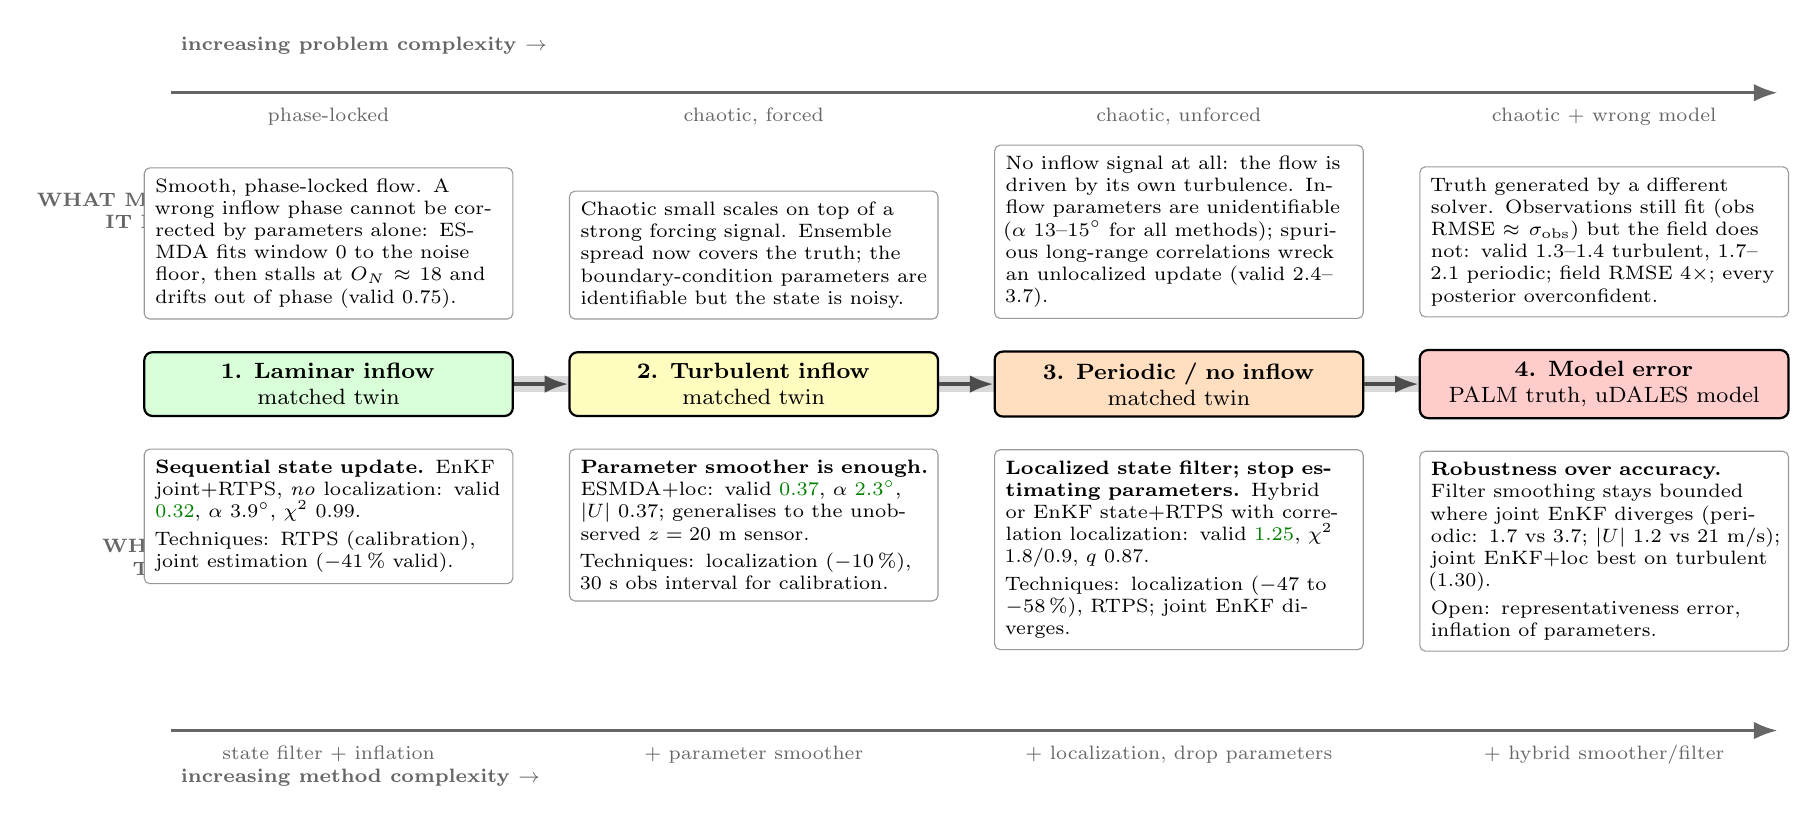
\begin{tikzpicture}[
  font=\footnotesize,
  station/.style={draw, rounded corners=3pt, fill=#1, minimum width=4.6cm, text width=4.4cm, align=center, inner sep=4pt, thick},
  card/.style={draw=black!40, rounded corners=2pt, fill=white, text width=4.4cm, align=left, inner sep=4pt, font=\scriptsize},
  lab/.style={font=\scriptsize\bfseries, text=black!60, align=right},
  arr/.style={-{Latex[length=3mm]}, line width=1.4pt, black!70},
]
% road
\draw[line width=6pt, black!15, rounded corners=8pt] (0,0) -- (5.4,0) -- (10.8,0) -- (16.2,0);
% stations
\node[station=green!15]  (s1) at (0,0)    {\textbf{1. Laminar inflow}\\matched twin};
\node[station=yellow!25] (s2) at (5.4,0)  {\textbf{2. Turbulent inflow}\\matched twin};
\node[station=orange!25] (s3) at (10.8,0)  {\textbf{3. Periodic / no inflow}\\matched twin};
\node[station=red!20]    (s4) at (16.2,0) {\textbf{4. Model error}\\PALM truth, uDALES model};
\foreach \a/\b in {s1/s2, s2/s3, s3/s4} \draw[arr] (\a) -- (\b);
% problem cards (above)
\node[lab, anchor=east] at (-1.3,2.2) {WHAT MAKES\\IT HARD};
\node[card, above=0.4cm of s1] (p1) {Smooth, phase-locked flow. A wrong inflow phase cannot be corrected by parameters alone: ESMDA fits window~0 to the noise floor, then stalls at $O_N\approx 18$ and drifts out of phase (valid 0.75).};
\node[card, above=0.4cm of s2] (p2) {Chaotic small scales on top of a strong forcing signal. Ensemble spread now covers the truth; the boundary-condition parameters are identifiable but the state is noisy.};
\node[card, above=0.4cm of s3] (p3) {No inflow signal at all: the flow is driven by its own turbulence. Inflow parameters are unidentifiable ($\alpha$ 13--15$^\circ$ for all methods); spurious long-range correlations wreck an unlocalized update (valid 2.4--3.7).};
\node[card, above=0.4cm of s4] (p4) {Truth generated by a different solver. Observations still fit (obs RMSE $\approx\sigma_{\rm obs}$) but the field does not: valid 1.3--1.4 turbulent, 1.7--2.1 periodic; field RMSE 4$\times$; every posterior overconfident.};
% remedy cards (below)
\node[lab, anchor=east] at (-1.3,-2.2) {WHAT IT\\TAKES};
\node[card, below=0.4cm of s1] (r1) {\textbf{Sequential state update.} EnKF joint$+$RTPS, \emph{no} localization: valid \good{0.32}, $\alpha$ 3.9$^\circ$, $\chi^2$ 0.99.\\[2pt]Techniques: RTPS (calibration), joint estimation ($-$41\,\% valid).};
\node[card, below=0.4cm of s2] (r2) {\textbf{Parameter smoother is enough.} ESMDA$+$loc: valid \good{0.37}, $\alpha$ \good{2.3$^\circ$}, $\Umag$ 0.37; generalises to the unobserved $z=20$ m sensor.\\[2pt]Techniques: localization ($-$10\,\%), 30 s obs interval for calibration.};
\node[card, below=0.4cm of s3] (r3) {\textbf{Localized state filter; stop estimating parameters.} Hybrid or EnKF state$+$RTPS with correlation localization: valid \good{1.25}, $\chi^2$ 1.8/0.9, $q$ 0.87.\\[2pt]Techniques: localization ($-$47 to $-$58\,\%), RTPS; joint EnKF diverges.};
\node[card, below=0.4cm of s4] (r4) {\textbf{Robustness over accuracy.} Filter smoothing stays bounded where joint EnKF diverges (periodic: 1.7 vs 3.7; $\Umag$ 1.2 vs 21 m/s); joint EnKF$+$loc best on turbulent (1.30).\\[2pt]Open: representativeness error, inflation of parameters.};
% method complexity axis
\draw[-{Latex[length=3mm]}, line width=1pt, black!60] (-2.0,-4.4) -- (18.4,-4.4); \node[font=\scriptsize\bfseries, black!60, anchor=west] at (-2.0,-5.0) {increasing method complexity $\rightarrow$};
\node[font=\scriptsize, black!60] at (0,-4.7)    {state filter $+$ inflation};
\node[font=\scriptsize, black!60] at (5.4,-4.7)  {$+$ parameter smoother};
\node[font=\scriptsize, black!60] at (10.8,-4.7)  {$+$ localization, drop parameters};
\node[font=\scriptsize, black!60] at (16.2,-4.7) {$+$ hybrid smoother/filter};
\draw[-{Latex[length=3mm]}, line width=1pt, black!60] (-2.0,3.7) -- (18.4,3.7); \node[font=\scriptsize\bfseries, black!60, anchor=west] at (-2.0,4.3) {increasing problem complexity $\rightarrow$};
\node[font=\scriptsize, black!60] at (0,3.4)    {phase-locked};
\node[font=\scriptsize, black!60] at (5.4,3.4)  {chaotic, forced};
\node[font=\scriptsize, black!60] at (10.8,3.4)  {chaotic, unforced};
\node[font=\scriptsize, black!60] at (16.2,3.4) {chaotic $+$ wrong model};
\end{tikzpicture}
\end{adjustbox}
\caption{Storyboard. Left to right the problem gets harder (top axis); each station lists
what makes it hard (top card) and the minimum method that copes with it (bottom card),
so that the bottom axis is the method-complexity ladder. Numbers are validation vector
RMSE [m/s], inflow-angle RMSE and calibration from Section~\ref{sec:cmp}.}
\label{fig:concl:story}
\end{figure}
\end{landscape}

\subsection{Bottom line}
\begin{enumerate}[nosep]
  \item \textbf{No single method wins.} The ranking of ESMDA, joint EnKF and the hybrid on
        held-out sensors reverses between the three regimes; the regime, not the knob,
        decides.
  \item \textbf{Parameters are recoverable only when an inflow signal exists}, and
        $\Umag$ only by the smoother-based methods (ESMDA, hybrid).
  \item \textbf{Localization and inflation are regime-dependent tools}: mandatory on
        periodic, neutral on turbulent inflow, harmful on laminar inflow (localization).
  \item \textbf{Calibration and accuracy are anti-correlated across methods}: the
        RTPS filters are calibrated ($\chi^2\approx1$) but not the most accurate; ESMDA
        and the hybrid are most accurate on turbulent inflow but overconfident.
  \item \textbf{Model error is the real frontier}: it compresses all methods to
        valid $\approx$1.3--1.4 and makes every posterior overconfident; the hybrid is
        the only method that never diverges under it.
\end{enumerate}


\end{document}
